\documentclass[11pt]{article}

% ---------------------------------------------------------------------------
% CONVENTIONAL-LAYOUT REWRITE (started 2026-07-19, per PI instruction).
% Layout: Abstract / Introduction / Related Work / Methodology (subsections) /
% Experiments / Results and Discussion / Conclusion.
% Writing rules (PI): plain academic prose, no em-dashes, no unproved claims,
% observational framing. Numbers only from data/key_numbers.md sections 18-19
% and the reconciled round-5 manuscript.
% Status 2026-07-19 (3rd pass): full draft. All sections written (Abstract,
% Introduction, Related Work, Methodology, Experiments, Results and Discussion,
% Conclusion, Limitations) plus appendices (details, exhibits, CLoRA
% cross-check). Grand results table = tables/table_grand.tex (all four metrics,
% error bars; overheads in appendix tab:cost).
% ---------------------------------------------------------------------------

\usepackage[review]{acl}
\usepackage{times}
\usepackage{latexsym}
\usepackage[T1]{fontenc}
\usepackage[utf8]{inputenc}
\usepackage{microtype}
\usepackage{inconsolata}
\usepackage[final]{graphicx}
\usepackage{booktabs}
\usepackage{amsmath,amssymb}
\usepackage{amsfonts}
\usepackage{xcolor}
\usepackage{colortbl} % cell shading in tables/table_geometry_battery.tex

\graphicspath{{figures/}}

% Let the tall full-width results table (a two-column table* float) sit at the
% top of a page near where it is referenced, instead of being deferred to the
% end of the document.
\renewcommand{\dbltopfraction}{0.9}
\renewcommand{\dblfloatpagefraction}{0.8}

\newcommand{\dw}{F_{\Delta}}
\newcommand{\smax}{\sigma_{\max}}

\title{What Governs Catastrophic Forgetting in Parameter-Efficient
Fine-Tuning?}

\author{Anonymous}

\begin{document}
\maketitle

% ===========================================================================
\begin{abstract}
% ===========================================================================
Many parameter-efficient fine-tuning (PEFT) adapters aim to preserve a
pretrained model's general capabilities, often by controlling where the
weight update lands. Each was introduced under its own forgetting protocol,
so the designs have not been compared on common ground. We evaluate five
retention-aware adapters and three reference arms on Llama-2-7B and
Qwen2.5-7B, across commonsense and math tuning, sweeping all but one over a
seven-point learning-rate grid with multiple seeds. This yields a pool of
$1{,}035$ runs evaluated under a common procedure for adaptation, retention,
update magnitude, geometry, and KL drift. Across $25$ Holm-corrected
comparisons, no adapter significantly outperforms plain LoRA with weight
decay. Beyond this head-to-head result, the shared measurement reveals the
dynamics behind retention: update magnitude strongly predicts it (pooled
$r=-0.847$), while geometry identifies the designs that constrain the
update but adds little predictive power once magnitude is known. The
learning rate affects retention through the update magnitude it produces,
so comparisons at a single shared rate partly reflect how well that rate
suits each method. Finally, retention benchmarks degrade in the same order
across all settings, so reported forgetting depends on the benchmark used
to measure it.
\end{abstract}

% ===========================================================================
\section{Introduction}\label{sec:intro}
% ===========================================================================
Catastrophic forgetting, the erosion of a pretrained model's general
capabilities when it is fine-tuned on a narrow task, is an obstacle to deploying adapted large language models. Parameter-efficient fine-tuning
(PEFT), and in particular LoRA~\citep{hu2021lora}, was expected to reduce it:
restricting the update to a low-rank correction $\Delta W = BA$ leaves the
bulk of the pretrained weights untouched. Forgetting nonetheless persists, and
a family of adapters has grown up to address it, choosing which directions to protect in the singular basis of the pretrained weight, in a calibration-data covariance basis, or through an orthogonality penalty (Section~\ref{sec:related}). These designs share the premise that where the update lands governs retention.

\paragraph{The gap.} Three things make it hard to know whether that premise
holds. First, each adapter was introduced under its own benchmarks and its own
notion of forgetting, so their retention numbers are not comparable:
CLoRA~\citep{clora} reports reasoning benchmarks, the data-aware methods
closed-book factoid QA, MiLoRA a language-modeling loss, and PiSSA and DoRA no
forgetting metric at all. Second, PEFT results vary strongly with the learning
rate and the random seed, so a comparison that does not tune each method
separately cannot separate what a design contributes from how well it happens
to be tuned. Third, the size of the update is a candidate that no comparison of
these adapters has tested, although published work points at it from outside
that comparison (Section~\ref{sec:related}). What is missing is the
measurement that would decide it: one retention axis and one magnitude axis,
with each method tuned at its own rate. We therefore include LoRA with weight
decay (LoRA{+}wd), plain LoRA with one knob aimed at the magnitude alone,
as the reference baseline.

\paragraph{This work.} We bring the adapters onto one measurement. Every
adapter is tuned in a single training harness and scored under four metrics
computed identically for all of them: the adaptation-retention operating
point, the update's magnitude (CLoRA's $\mathbb{F}$ diagnostic, which we
adopt as a method-neutral magnitude axis $\dw$), its geometry relative to the
base weight's spectrum, and its KL drift from the base model
(Section~\ref{sec:method:metrics}). Each method is swept over seven learning
rates and multiple seeds, across two architectures (Llama-2-7B and
Qwen2.5-7B) and two task types (commonsense and math), giving a frozen pool
of $1{,}035$ trained adapters.
Against this pool we ask four questions:
\begin{itemize}
  \item \textbf{RQ1.} Compared under one protocol and swept over rates and seeds, is any retention-aware adapter significantly better than a plain magnitude control (LoRA with adapter weight decay), in adaptation or retention?
  \item \textbf{RQ2.} What governs the adaptation-retention outcome: the
  magnitude of the update, or the subspace it lands in?
  \item \textbf{RQ3.} Can the KL drift serve as a practical retention monitor?
  \item \textbf{RQ4.} Do retention benchmarks degrade in the same order as forgetting progresses?
\end{itemize}
Our contributions are: (i) a common measurement for the retention-aware
adapter family, eight LoRA-family adapters (with DoRA as a reparameterization
baseline and LoRA{+}wd as the magnitude-only control) under four identically
computed metrics, swept over rates and seeds, with cluster-robust,
multiplicity-corrected inference; (ii) a frozen pool of $1{,}035$ trained
adapters with their per-run metrics and the statistics behind every exhibit,
released so that the analyses here can be re-run and extended; and (iii) four
measured answers, that no adapter is significantly better than a plain
magnitude control, that retention tracks the size of the update while its
placement in the base weight's spectrum adds far less, that KL drift serves as
a retention monitor, and that the retention benchmarks degrade in one fixed
order.

\paragraph{What we observe.} Brought onto one measurement, the premise does
not hold up. No adapter is significantly better than LoRA{+}wd on either
axis, and at matched update magnitude the only departures from it are
deficits: five of the seven swept adapters are equivalent to the control
within $\pm3$ retention points, and the two that are not, PiSSA and
SC-LoRA, fall $7.1$ and $4.1$ points below it. What separates runs is how
large the update is, not where it lands: magnitude predicts retention at
pooled $r=-0.847$, while geometry adds $+0.017$ of $R^2$ and method
identity $+0.006$ once magnitude is known. Because different adapters turn
the same learning rate into different magnitudes, a comparison at one
shared rate partly measures how well that rate suits each method; the
per-method sweep removes this.

% ===========================================================================
\section{Related Work}\label{sec:related}
% ===========================================================================
\paragraph{Retention-aware PEFT adapters.} These adapters share a geometric
premise, and in this literature the geometry of an update means one specific
thing: the pretrained weight comes with an ordering of directions, its major
components at one end and its minor components at the other, and a design
decides at which end the update is placed. The ordering is read either from
the singular value decomposition of the weight itself or from the second
moment of the activations a calibration corpus produces, and the designs
differ mainly in which end they select. PiSSA~\citep{meng2024pissa} places the
update in the major components and SC-LoRA~\citep{luo2025sclora} in the major
directions of the output second moment; MiLoRA~\citep{wang2024milora} places
it in the minor components and LoRA-Null~\citep{tang2025loranull} in the least
activated input directions; CorDA~\citep{yang2024corda} and
CorDA++~\citep{yang2025cordapp} select in a context-oriented decomposition; and
OPLoRA~\citep{xiong2025oplora} withholds it from the major subspace
altogether. Our geometry coordinates measure that placement directly, as the
share of the update's energy in the major and the minor singular subspaces of
the base weight on the input and the output side
(Section~\ref{sec:method:metrics}). A separate group falls outside this
construct, constraining the update with an orthogonality penalty against a
subspace that is not ordered by size: O-LoRA~\citep{wang2023olora} learns each
new task in a subspace orthogonal to previously learned ones, and
CLoRA~\citep{clora} generalizes the penalty to one-stage fine-tuning against a
fixed subspace, with the stated premise that forgetting tracks the scale of
the induced output change rather than where the update lands. DoRA~\citep{liu2024dora} targets adaptation quality and
makes no retention claim; we include it as a widely used reparameterization
baseline. We evaluate one representative per group (PiSSA and MiLoRA;
SC-LoRA and LoRA-Null; CLoRA).
CLoRA supplies the experimental frame we build on: it reports forgetting on
the benchmarks we use, it introduced the magnitude diagnostic we adopt as
$\dw$, our dense Llama grids start from its published configuration, and
its published numbers recur as external corroboration of ours
(Appendix~\ref{app:clora}). We widen that frame to the whole family: the
same protocol over all the adapters, asking whether geometry adds anything
beyond magnitude and whether plain LoRA{+}wd reaches the same operating
points at matched capacity.

\paragraph{Update size.} Continual learning typically either penalizes
movement away from previous weights or replays stored
data~\citep{wang2024clsurvey,rolnick2019replay}; the adapter family we study
does neither. The link between weight movement and forgetting is
longstanding: EWC~\citep{kirkpatrick2017ewc} and L$^2$-SP~\citep{li2018l2sp}
penalize distance from the pretrained weights directly,
\citet{kalajdzievski2024scaling} fits scaling laws in which forgetting grows
with the parameters tuned and the steps taken, and \citet{biderman2024lora}
report that LoRA forgets less than full fine-tuning while also learning
less. Recent work points at update magnitude as the quantity behind these
observations. \citet{zhang2025primacy} treat the learning rate, the scaling
factor, and the initialization as three controls on update magnitude, and
attribute spectral initialization's advantage to the magnitude it induces
rather than to its directions, though for adaptation quality rather than
retention. \citet{huang2025fapm} prune adapters by the size of the update
relative to the pretrained weight, \citet{koubbi2026meanfield} derive a
sharp transition from a non-forgetting to a forgetting regime as the
perturbation grows, and single-method reports within the adapter family
point the same way~\citep{wang2024milora,tang2025loranull}. None of this
work measures magnitude against placement across the retention-aware
family; that comparison is what our protocol adds.

\paragraph{Update geometry.} \citet{shuttleworth2025illusion} read fine-tuned
weights on a different coordinate, the spectrum of the adapted matrix
$W_0{+}\Delta W$: LoRA introduces new leading singular directions
near-orthogonal to the pretrained ones, and scaling them down after training
improves modeling of the pretraining distribution at a small cost in task
accuracy. That coordinate is a property of the resulting weight rather than a place a
design puts its update, so it lies outside the construct above, and their
outcome is the pretraining distribution rather than benchmark retention, so
nothing we measure tests their claim. Their lever also
moves with ours, since raising the rate or the scaling factor both enlarges
the update and adds those directions, so the two studies read the same
lever on different coordinates. Concurrent work presses the same point from
the other side: \citet{xie2026intruder} derive a per-layer critical update
strength from the base spectrum and report norm-matched interventions in which
threshold-crossing layers, rather than update size, carry the forgetting.
Their unit is the layer and their coordinate is the adapted spectrum; ours is
the adapter and the placement of $\Delta W$, measured across methods at
equalized tuning, so the two measurements can disagree without either being
wrong, and reconciling them is the natural next experiment (Limitations).

\paragraph{Tuning as a confound.} \citet{lee2026lr} sweep the rate per method
and find that peak \emph{adaptation} converges across several LoRA variants;
we reach the analogous conclusion for retention and trace it to the magnitude
each rate produces (Section~\ref{sec:results:rq2}). What none of this work does is place the
adapter family on one retention measurement with a common magnitude axis, so
none of it can ask whether the adapters differ once tuning is equalized (RQ1)
or how far geometry adds to magnitude within the family (RQ2).

% ===========================================================================
\section{Measurement setup}\label{sec:method}
% ===========================================================================

%% agent: from here
%% agent: to here - all this section more relevant to the introduction. Here we should focus on what we offer or contribute here to fix it
%% CLAUDE: done - deleted the gap restatement (it already lives in the
%% Introduction's "The gap" paragraph) and opened directly with what we build.
We built one common measurement for the retention-aware adapter family: a
unified reimplementation of the designs of Section~\ref{sec:related} with
standard reference methods, a protocol that sweeps learning rates and seeds
per method, and four metrics computed identically for every trained adapter.

% ---------------------------------------------------------------------------
\subsection{Adapters under study}\label{sec:method:adapters}
% ---------------------------------------------------------------------------
All methods build on LoRA~\citep{hu2021lora}, which adds a trainable low-rank
correction $\Delta W = BA$ to selected frozen weight matrices, and constrain or
initialize that correction in the ways set out in Section~\ref{sec:related}. We
compare them against plain LoRA, DoRA~\citep{liu2024dora}, which makes the
update's magnitude an explicitly learned quantity, and LoRA with weight decay
(LoRA{+}wd), plain LoRA with AdamW weight decay on the adapter matrices, which
needs no initialization pass or auxiliary loss and is the simplest possible
magnitude control. Its decay was set once before the campaign and not revisited,
and it is swept in its own right in the two grid settings alongside CLoRA's
subspace dimension and LoRA's rank (Appendix~\ref{app:sweep}).

Every adapter is implemented from its original paper inside one training loop
and evaluated under one protocol. The sweep is what makes the comparison fair,
because the same rate becomes a very different update magnitude under different
initializations (Section~\ref{sec:results:rq2}). We therefore sweep the same
seven-point rate grid for every method except PiSSA, which enters at its recipe
rate only, report each at its own best-adaptation rate over up to five seeds per
cell, and add two controls: an eval-matched calibration for the data-aware
initializations (Appendix~\ref{app:sweep}) and a parameter-matched
LoRA{+}wd at plain LoRA's rank (Section~\ref{sec:results:rq1}). Per-method configurations, coverage and the
full protocol are in Appendix~\ref{app:details}.

% ===========================================================================
\subsection{Data, models and scale}\label{sec:method:setup}
% ---------------------------------------------------------------------------
We fine-tune Llama-2-7B~\citep{touvron2023llama2} and
Qwen2.5-7B~\citep{qwen2025qwen25} on commonsense reasoning, with the eight-task
LLM-Adapters suite~\citep{hu2023llmadapters}, and on mathematics, with
MetaMathQA~\citep{yu2023metamath} evaluated on GSM8K~\citep{cobbe2021gsm8k}:
four model $\times$ task settings. Adaptation is mean accuracy over the eight
commonsense tasks (CS-8) or GSM8K exact match. Core retention is the mean of two
held-out benchmarks the fine-tuning data does not touch,
BBH~\citep{suzgun2023bbh} and MMLU-Pro~\citep{wang2024mmlupro}; without
fine-tuning core retention stands at $26.0$ on Llama-2-7B and $44.4$ on
Qwen2.5-7B. In the math settings it is BBH alone,
because MetaMath-tuned models answer MMLU-Pro in a format our parser does not
reliably extract, a parsing artifact rather than forgetting.
MMLU~\citep{hendrycks2021mmlu}, ARC-Challenge~\citep{clark2018arc} and
TruthfulQA~\citep{lin2022truthfulqa} are scored on every run but stay out of
headline retention, and retention runs the
lm-evaluation-harness~\citep{evalharness} on full benchmark sets without
subsampling.

Six to eight adapters run over the shared rate grid in each setting, three seeds
per configuration by default. On Llama we add two denser grids that hold the
training recipe fixed and vary one magnitude knob instead, weight decay,
CLoRA's $k$, or LoRA rank, for the analyses of Section~\ref{sec:results:rq2};
they start from CLoRA's published configuration, which we thereby also
reproduce (Appendix~\ref{app:clora}). Together they form the frozen analysis pool of
$1{,}035$ adapters over $344$ configurations; rosters, seed coverage, knob
ranges and inclusion rules are in Appendix~\ref{app:details}. The experimental
stack, the pool and the statistics scripts behind every exhibit will be
released.

% ---------------------------------------------------------------------------
\subsection{Metrics}\label{sec:method:metrics}
% ---------------------------------------------------------------------------
For every trained adapter we compute four measurements. The first is the
outcome pair the adapters are designed to improve; the remaining three are
candidate explanations for it, one per axis raised in the prior literature.

\paragraph{Metric 1: operating points.} Adaptation is
accuracy on the fine-tuning task's evaluation suite; retention is accuracy on
held-out general benchmarks that the fine-tuning data does not cover
(Section~\ref{sec:method:setup} lists both). For each method we consider its
swept operating points (cell means over seeds) in the adaptation-retention
plane and report the observed retention-adaptation frontier, so methods are
compared as frontiers rather than as single configurations.

\paragraph{Metric 2: update magnitude.} Our magnitude measure is the mean
normalized output displacement the update induces on real token traffic, the
average of $\lVert \Delta W_\ell\, x \rVert_2 / \lVert x \rVert_2$ over every
adapted module $\ell$ and every token of a fixed probe set, which is CLoRA's
$\mathbb{F}$ diagnostic~\citep{clora}. The update $\Delta W_\ell$ includes any
initialization residual, so a zero-step run gives $\Delta W = 0$; the probe set,
the hooks and the exact expression are in Appendix~\ref{app:metrics}. We prefer
$\dw$ over the Frobenius and spectral norms because it is activation-weighted,
measuring how much the update actually displaces the model's outputs, and it is
empirically the strongest of ten candidate measures
(Table~\ref{tab:league}, Appendix~\ref{app:exhibits}).

\paragraph{Metric 3: update geometry.} We measure the placement of
Section~\ref{sec:related}, the end of the base weight's spectrum the update
occupies, on the trained adapters themselves.
Each saved update $\Delta W = (\alpha/r)BA$ is compared against the singular
value decomposition of the corresponding base weight $W_0$. On the output
side, we project the update's singular directions, weighted by their singular
values, onto the major (top-$256$) and minor (bottom-$256$) left singular
subspaces of
$W_0$ (exact computation in Appendix~\ref{app:geoproj}),
giving the energy fractions $e_{\mathrm{top}}$ and $e_{\mathrm{bot}}$;
the same projection on the input side, against the right singular subspaces,
gives $e^{\mathrm{in}}_{\mathrm{top}}$ and $e^{\mathrm{in}}_{\mathrm{bot}}$.
We also compute the update's stable rank,
$\lVert\Delta W\rVert_F^2 / \smax^2$ with $\smax$ the largest singular
value of $\Delta W$: the number of directions that effectively carry the
update (near $1$ when a single direction dominates).
The four energy shares are the placement of Section~\ref{sec:related},
measured at a fixed boundary of $256$ directions; the stable rank describes
the update's shape and is not a placement measure.

\paragraph{Metric 4: KL drift.} In the spirit of the loss-drift
proxies of \citet{wang2024milora} and \citet{kalajdzievski2024scaling}, we
measure the cross-entropy of the adapted model to its base on held-out
neutral text (the WikiText-103 test set)~\citep{merity2017wikitext}; since CE and KL to base differ only by the base model's entropy
(a per-model constant), we quote the KL form.

% ===========================================================================
\section{Results}\label{sec:results}
% AUTO-GENERATED by acl_analysis/rq1_stats/06_make_grand_compact.py:
% column-trimmed copy of the frozen table_grand.tex (numbers verbatim).
% Do not hand-edit numbers.
\begin{table*}[t]
\centering
\footnotesize
\setlength{\tabcolsep}{3pt}
% two half-tables side by side (Llama | Qwen) so the float fits one
% page-width band and places early.
\begin{minipage}[t]{0.49\textwidth}\centering
\begin{tabular}{l | cc | cc}
\toprule
\textbf{Method} & \textbf{Ret} $\uparrow$ & \textbf{Adapt} $\uparrow$ & $\dw$ $\downarrow$ & \textbf{KL} $\downarrow$ \\
\midrule
\multicolumn{5}{c}{\textbf{Llama-2-7B, commonsense}} \\
\midrule
\textit{Base model} & \textit{26.0} & -- & \textit{0} & \textit{0} \\
LoRA+wd & \textbf{25.9{\footnotesize$\pm$0.4}} & \textbf{81.8{\footnotesize$\pm$0.2}} & 0.40{\footnotesize$\pm$0.01} & \textbf{0.19{\footnotesize$\pm$0.00}} \\
SC-LoRA\smash{$^{\ast}$} & 24.6{\footnotesize$\pm$1.9} & 80.6{\footnotesize$\pm$0.4} & \textbf{0.38{\footnotesize$\pm$0.16}} & 0.21{\footnotesize$\pm$0.09} \\
LoRA & 23.9{\footnotesize$\pm$0.5} & 79.2{\footnotesize$\pm$0.2} & 0.62{\footnotesize$\pm$0.01} & 0.42{\footnotesize$\pm$0.03} \\
LoRA-Null & 21.8{\footnotesize$\pm$1.3} & 78.9{\footnotesize$\pm$0.2} & 0.70{\footnotesize$\pm$0.00} & 0.56{\footnotesize$\pm$0.03} \\
CLoRA & 21.6{\footnotesize$\pm$0.4} & 78.3{\footnotesize$\pm$0.2} & 0.65{\footnotesize$\pm$0.01} & 0.64{\footnotesize$\pm$0.02} \\
MiLoRA & 21.4{\footnotesize$\pm$0.9} & 77.2{\footnotesize$\pm$0.4} & 0.85{\footnotesize$\pm$0.01} & 0.74{\footnotesize$\pm$0.01} \\
DoRA & 19.1{\footnotesize$\pm$1.4} & 76.2{\footnotesize$\pm$1.6} & 1.23{\footnotesize$\pm$0.02} & 0.71{\footnotesize$\pm$0.01} \\
\midrule
\multicolumn{5}{c}{\textbf{Llama-2-7B, math}} \\
\midrule
\textit{Base model} & \textit{33.1} & -- & \textit{0} & \textit{0} \\
LoRA+wd & \textbf{33.6{\footnotesize$\pm$1.0}} & \textbf{66.8{\footnotesize$\pm$0.8}} & \textbf{0.28{\footnotesize$\pm$0.00}} & \textbf{0.23{\footnotesize$\pm$0.00}} \\
MiLoRA & 32.4{\footnotesize$\pm$0.1} & 63.7{\footnotesize$\pm$0.8} & 0.45{\footnotesize$\pm$0.00} & 0.67{\footnotesize$\pm$0.03} \\
LoRA & 31.3{\footnotesize$\pm$0.3} & 64.0{\footnotesize$\pm$0.9} & 0.44{\footnotesize$\pm$0.01} & 0.52{\footnotesize$\pm$0.02} \\
LoRA-Null & 28.9{\footnotesize$\pm$0.6} & 61.9{\footnotesize$\pm$0.6} & 0.89{\footnotesize$\pm$0.01} & 1.26{\footnotesize$\pm$0.03} \\
CLoRA & 28.6{\footnotesize$\pm$0.1} & 60.6{\footnotesize$\pm$0.4} & 1.01{\footnotesize$\pm$0.01} & 1.40{\footnotesize$\pm$0.01} \\
DoRA & 28.1{\footnotesize$\pm$1.1} & 59.2{\footnotesize$\pm$0.5} & 2.85{\footnotesize$\pm$0.02} & 2.42{\footnotesize$\pm$0.43} \\
SC-LoRA & 27.9{\footnotesize$\pm$0.5} & 60.5{\footnotesize$\pm$0.5} & 0.86{\footnotesize$\pm$0.00} & 1.18{\footnotesize$\pm$0.02} \\
\bottomrule
\end{tabular}
\end{minipage}\hfill
\begin{minipage}[t]{0.49\textwidth}\centering
\begin{tabular}{l | cc | cc}
\toprule
\textbf{Method} & \textbf{Ret} $\uparrow$ & \textbf{Adapt} $\uparrow$ & $\dw$ $\downarrow$ & \textbf{KL} $\downarrow$ \\
\midrule
\multicolumn{5}{c}{\textbf{Qwen-2.5-7B, commonsense}} \\
\midrule
\textit{Base model} & \textit{44.4} & -- & \textit{0} & \textit{0} \\
LoRA+wd & \textbf{40.1{\footnotesize$\pm$0.7}} & \textbf{87.4{\footnotesize$\pm$0.2}} & 0.25{\footnotesize$\pm$0.00} & 0.23{\footnotesize$\pm$0.00} \\
CLoRA & 39.5{\footnotesize$\pm$1.1} & 87.0{\footnotesize$\pm$0.2} & 0.13{\footnotesize$\pm$0.00} & 0.13{\footnotesize$\pm$0.01} \\
LoRA-Null & 39.0{\footnotesize$\pm$0.7} & 86.2{\footnotesize$\pm$1.6} & 0.20{\footnotesize$\pm$0.01} & 0.21 \\
DoRA & 38.0{\footnotesize$\pm$1.0} & 86.4{\footnotesize$\pm$0.8} & 0.26{\footnotesize$\pm$0.00} & 0.28{\footnotesize$\pm$0.01} \\
LoRA & 38.0{\footnotesize$\pm$0.9} & 86.4{\footnotesize$\pm$0.4} & \textbf{0.12{\footnotesize$\pm$0.00}} & \textbf{0.07{\footnotesize$\pm$0.00}} \\
MiLoRA & 36.7{\footnotesize$\pm$0.1} & 86.4{\footnotesize$\pm$1.0} & 0.28{\footnotesize$\pm$0.01} & 0.48{\footnotesize$\pm$0.02} \\
SC-LoRA & 27.9{\footnotesize$\pm$16.0} & 87.2{\footnotesize$\pm$0.1} & 0.35{\footnotesize$\pm$0.08} & -- \\
\midrule
\multicolumn{5}{c}{\textbf{Qwen-2.5-7B, math}} \\
\midrule
\textit{Base model} & \textit{47.9} & -- & \textit{0} & \textit{0} \\
SC-LoRA & \textbf{47.7{\footnotesize$\pm$0.2}} & \textbf{77.2{\footnotesize$\pm$0.8}} & 0.11{\footnotesize$\pm$0.00} & 0.10{\footnotesize$\pm$0.00} \\
LoRA+wd & 47.5{\footnotesize$\pm$0.4} & 69.0{\footnotesize$\pm$3.3} & 0.10{\footnotesize$\pm$0.00} & -- \\
MiLoRA & 46.2{\footnotesize$\pm$1.3} & 65.3{\footnotesize$\pm$4.0} & 0.15{\footnotesize$\pm$0.01} & 0.27{\footnotesize$\pm$0.02} \\
LoRA & 46.1{\footnotesize$\pm$1.5} & 63.5{\footnotesize$\pm$4.3} & \textbf{0.07{\footnotesize$\pm$0.00}} & \textbf{0.05} \\
DoRA & 46.1{\footnotesize$\pm$0.7} & 63.9{\footnotesize$\pm$4.5} & 0.11 & -- \\
LoRA-Null & 44.8{\footnotesize$\pm$0.6} & 72.3{\footnotesize$\pm$1.3} & 0.39{\footnotesize$\pm$0.01} & 0.41 \\
CLoRA & 40.0{\footnotesize$\pm$0.1} & 70.5{\footnotesize$\pm$1.0} & 0.44{\footnotesize$\pm$0.01} & 0.73{\footnotesize$\pm$0.01} \\
\bottomrule
\end{tabular}
\end{minipage}
\caption{Each method at its best adaptation operating point, one block
per model and task, sorted by retention. Ret, Adapt, $\dw$, and KL are
mean $\pm$ SD over seeds. The full
version with the five geometry columns is Table~\ref{tab:grand-full}
(Appendix~\ref{app:exhibits}).}
\label{tab:grand}
\end{table*}

% ===========================================================================
\paragraph{How we test.} A \emph{cell} is one configuration of
Section~\ref{sec:method:setup}, so runs in a cell differ only in the random
seed; cells group into six \emph{run families}: the four learning-rate
sweeps, one per model $\times$ task setting, and the two denser Llama grids
of Section~\ref{sec:method:setup} that vary a magnitude knob at a fixed
recipe (family sizes in Appendix~\ref{app:pool}).
Seeds within a cell are correlated, so every test is cluster-robust at the
cell level or paired within cells, with Holm correction across the method
comparisons. The design detects retention effects of roughly two to five
points at typical cells and coarser ones on Qwen (Table~\ref{tab:mde}).
Run conventions, exclusions, and scope notes are in
Appendix~\ref{app:pool}.

% ---------------------------------------------------------------------------
\subsection{No adapter is significantly better than plain LoRA with weight decay}\label{sec:results:rq1}
% ---------------------------------------------------------------------------

\paragraph{Operating points and corrected tests.} Table~\ref{tab:grand} reports
every swept method at its best-adaptation operating point. LoRA{+}wd is the top-retaining method in
three of the four settings and trails the leader by $0.17$ points in the
fourth, while sitting at or near the top of the adaptation column in each
Llama block. At those operating points we ran $26$ method $\times$ setting
comparisons against LoRA{+}wd with paired per-seed $t$ tests; $25$ are
testable, and the one that is not, single-seed PiSSA on Llama math, is far
below on both axes. After Holm correction,
\textbf{no method is significantly better than LoRA{+}wd on either axis}.
Two comparisons are significantly worse on retention and five on
adaptation, by $2.6$ to $7.6$ points; every delta, CI, and corrected $p$ is
in Appendix~\ref{app:head2head}. These are within-harness comparisons at
matched capacity; they do not bear on the published CLoRA results, which
our faithful-recipe replication treats as the reference point
(Appendix~\ref{app:clora}).

\paragraph{Equivalence bounds.} An equivalence test (TOST) asks whether each
method's retention offset from LoRA{+}wd at matched update magnitude stays
inside a margin of $3$ points: five of the seven adapters do. The two that
fail lie below the reference, PiSSA at $-7.1$ points and SC-LoRA at $-4.1$
(specification and tighter margins in Table~\ref{tab:tost}; PiSSA's
single-rate scope note in Appendix~\ref{app:configs}). Differences below
about $2$ points remain open at this design's power.

\paragraph{The capacity control.} Ranks are not matched across methods
(Appendix~\ref{app:configs}), so LoRA{+}wd's edge could come simply from more
trainable parameters. Two controls say otherwise. LoRA{+}wd retrained at
rank $16$, plain LoRA's parameter count, reproduces the reference's
retention and update size over five seeds ($26.61\!\pm\!0.23$ at
$\dw\!=\!0.347\!\pm\!0.014$, against $25.9\!\pm\!0.4$ at $0.40$), though one
of the five seeds collapses on the adaptation suite ($74.6\!\pm\!13.0$
against the rank-$32$ arm's $81.8\!\pm\!0.2$). And raising plain LoRA's rank
at the fixed standard rate buys no retention: it grows the update and slides
the run \emph{down} the shared curve. Parameter count matters only through
the update magnitude it produces.

\paragraph{The one suggestive reversal.} One comparison of the $26$ runs
the other way: SC-LoRA on Qwen math reaches GSM8K $77.2\!\pm\!0.8$, $8.26$
adaptation points above LoRA{+}wd at tied retention (BBH $+0.17$). It does
not survive correction (raw paired $p\!=\!0.035$,
$p_{\text{Holm}}\!=\!0.21$), so we report it as suggestive. The winning cell
is low-magnitude ($\dw\!=\!0.107$), so SC-LoRA wins by adapting more at a
small update rather than by tolerating a large one. On Llama commonsense the
choice of SC-LoRA's calibration corpus alone moved it by about $4$ points,
so we attribute the gain to the data-aware initialization as configured; no
such control exists for Qwen math, and SC-LoRA is the study's most
seed-fragile method (Table~\ref{tab:grand}).

% ---------------------------------------------------------------------------
\subsection{Retention tracks update magnitude; geometry identifies the designs that constrain it}\label{sec:results:rq2}
% ---------------------------------------------------------------------------
Update magnitude is the strongest single predictor of retention in the study,
and the prediction is robust to how the update was produced. The geometry is
shaped by each design clearly enough to identify the method from its trained
weights, but where the update lands adds little once magnitude is known.

\paragraph{Magnitude predicts retention.} Figure~\ref{fig:hero} plots
core retention against the effective update magnitude $\dw$ on Llama-2-7B
commonsense: adapters of all designs
interleave along a single downward curve. Pooled over all
$1{,}035$ runs, the correlation with $\log_{10}\dw$ is $-0.847$, and within every one of the six run families, it is
$-0.830$ to $-0.929$; the corresponding plot for each family is in Figure~\ref{fig:family-scatter} (Appendix~\ref{app:exhibits}). Within-cell
seed scatter is $0.3$--$2.7$ points against the roughly $20$ to $40$ points each family's retention spans, from which we conclude that the relation reflects the update magnitude rather than run-to-run noise. \\ 
The curve is knee-shaped: retention is flat while $\dw$ stays below a per-family threshold (the \emph{knee}) and, once $\dw$ exceeds that threshold, falls
by $7.5$ to $40.8$ points per decade of $\dw$, one shared shape with per-family constants (fit details in Appendix~\ref{app:exhibits}). \\
The adaptation peaks at the retention knee and
falls beyond it, so training past the knee loses on both axes at once.

\begin{figure}[t]
  \centering
  
\includegraphics[width=0.74\columnwidth]{fig0_hero.png}
  \caption{Core retention (mean of BBH and MMLU-Pro) versus $\dw$ (log scale)
  for the $448$ Llama-2-7B commonsense runs in the frozen pool that fall inside the axes; The adapters of all
  designs interleave along one curve, and the knee is near
  $\dw \approx 0.4$. The star marks the LoRA{+}wd operating point of Table~\ref{tab:grand}.}
  \label{fig:hero}
\end{figure}

\paragraph{Not an artifact of the recipe.} Large updates usually come from
aggressive recipes, so the recipe rather than the update size could be what
destroys retention. Three checks say otherwise. First, holding the recipe
fixed, the chance differences in update size between runs that differ only
in seed still predict retention ($r\!=\!-0.713$, $954$ runs). Second,
changing the size with no training at all, $15$ rescaled adapters track the
curve of Figure~\ref{fig:hero}, while $9$ same-size updates in random
directions land $3.05$ points below them (Appendix~\ref{app:exhibits}).
Third, which knob produced the magnitude, weight decay, CLoRA's $k$, or
LoRA rank, adds at most $\Delta R^2 = 0.006$ once $\dw$ is known
(Figure~\ref{fig:dose}).

\paragraph{The learning rate acts through magnitude.} 
The trend of Figure~\ref{fig:hero} may simply reflect that larger learning rates cause greater retention loss. Thus, we tested which of the two variables carries the
signal on the existing pool of runs. First, we
compared runs trained at the same learning rate, which still differ in update magnitude through method, rank, weight decay,  and seed; among them, the magnitude still predicts retention within every grid rate at or above $10^{-4}$ in every family ($r \le -0.7$). Second, by controlling for the magnitude, the rate predicts almost nothing (partial correlation $-0.17$ to $+0.29$ per family), while controlling for the
rate, magnitude keeps most of its signal ($-0.58$ to $-0.91$). We conclude that learning rate affects retention through update magnitude. Consequently, a shared learning rate does not imply comparable update sizes across methods, so comparisons at a single rate may partly reflect how well that rate suits each method. We quantify this effect and each method's learning-rate sensitivity in Appendix~\ref{app:exhibits} (Figure~\ref{fig:lrartifact}) and Appendix~\ref{app:lrsweep}.

\paragraph{Geometry beyond magnitude.}If the update's size is already known, how much does knowing where it lands improve prediction of retention? We answer with a regression on the 1,034 pooled runs, adding predictor blocks sequentially and recording the increase in explained variance ($R^2$): run family explains $0.390$, update size adds $+0.395$, geometry adds only $+0.017$, and method identity adds $+0.006$ (Table~\ref{tab:ladder}). The result is not an artifact of this ordering: a variance decomposition attributes $+0.296$ uniquely to size versus only $+0.016$ uniquely to geometry, and size contributes more than geometry in all $2{,}000$ bootstrap replicates. Thus, once the update size is known, where the update lands adds little predictive power for retention. Further analyses, including coarser and placement-only decompositions, are reported in Appendix~\ref{app:exhibits}.

\begin{figure}[t]
\centering
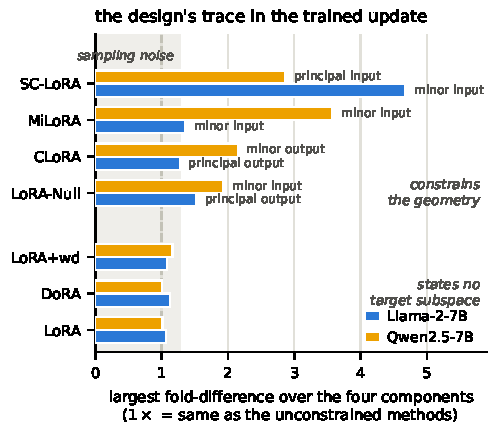
\includegraphics[width=\columnwidth]{fig_geometry_detect.pdf}
\caption{How far each method's update, at its Table~\ref{tab:grand}
operating point, sits from plain updates (LoRA, LoRA{+}wd, DoRA) trained at
the same learning rate. Each bar is the largest ratio across four measures
of where the update's energy lies; one means indistinguishable from plain,
and the shaded band is the $99$th percentile among the plain runs alone.
Labels name the measure that differs most, starred where the two base
models disagree.}
\label{fig:geometry}
\end{figure}

\paragraph{Geometry identifies the designs.}
The small geometry step does not mean that the constraints fail to shape the updates. Figure~\ref{fig:geometry} compares each method's trained update with plain updates trained at the same learning rate, using four measures of where the update's energy lies (computation in Appendix~\ref{app:geoproj}). Every method that constrains update geometry separates from the plain adapters on both base models (SC-LoRA, MiLoRA, and LoRA-Null), while the three plain methods remain within the band produced by resampling the plain runs. CLoRA is the exception, consistent with its constraint acting on a randomly drawn subspace that these measures do not capture. Because the measures are scale-invariant energy shares, they cannot reflect update magnitude by construction. Thus, the constraints clearly alter update geometry, but this geometric variation has limited predictive power for retention: after fitting retention on magnitude and method within each family, the remaining method differences reach about five points among the swept methods, compared with roughly $20$--$40$ points spanned by the magnitude relationship (Appendix~\ref{app:exhibits}).

\paragraph{Outside the family, the shape holds, but the level does not.}
Does the relation extend beyond LoRA-style adapters? We add three full
fine-tuning runs of the Llama commonsense setup, spanning small to large
updates. Retention decreases monotonically with $\dw$, so the shape of the
relationship extends beyond the adapter family. The level does not: all
three runs fall below the LoRA-family curve. Only one falls within the
magnitude range covered by the family, allowing a direct comparison without
extrapolation. At $\dw \approx 0.4$, it retains $17.1$, compared with a mean
of $25.6$ across the $72$ Llama commonsense family runs in the same magnitude
band, and below every one of them. We interpret this gap as an upper bound:
$\dw$ measures changes only in the five weight matrices targeted by the
adapters, whereas full fine-tuning updates all parameters. Its true update
is therefore larger than the measured one, and the family curve would be
lower at that larger magnitude. Thus, the curve's absolute level should be
interpreted as a within-family result.

% ---------------------------------------------------------------------------
\subsection{KL drift tracks retention and needs no benchmark run}\label{sec:results:rq3}
% ---------------------------------------------------------------------------
Following the loss-drift proxy of
MiLoRA~\citep{wang2024milora}, we measure the KL divergence from the
adapted model's next-token distribution to the base model's on held-out
text (Metric 4, Section~\ref{sec:method:metrics}). It is the same signal
as magnitude, correlating with retention at $-0.63$ to $-0.92$ per run
family while adding only $+0.005$ of retention variance beyond magnitude,
against magnitude's $+0.085$ beyond it. What makes it useful is its cost:
one forward pass, no benchmark harness, no adapter weights. On Llama it
can stand in for the benchmark, a per-family curve converting drift into
predicted retention to within $1.3$--$2.0$ points on cells the fit never
saw (Figure~\ref{fig:ceproxy}); on Qwen the estimate is coarser, off by
roughly $4$--$6$ points, but drift still flags damaged runs in all six run
families, and drift and magnitude both identify which cells will be
unstable across seeds before any benchmark is run (detection statistics,
two qualifications, and the instability result in
Appendix~\ref{app:exhibits}).

% ---------------------------------------------------------------------------
\subsection{Retention benchmarks degrade in a fixed order}\label{sec:results:rq4}
% ---------------------------------------------------------------------------
Ranked by how quickly accuracy declines as the update grows, normalized by
each benchmark's base score, MMLU-Pro is the most sensitive, followed by
BBH, MMLU, and TruthfulQA. On the four Llama run families, TruthfulQA
actually \emph{improves}, so we report the broad retention aggregate both
with and without it. This ordering is highly consistent: it is identical
across all six run families, spanning both models and both tasks
(Kendall's $W=1.000$, indicating perfect agreement; the corresponding
$p$-values are $4.4\times10^{-4}$ when treating the six families as
independent and $0.0074$ when treating the four distinct model-by-task
settings as the independent units; see Table~\ref{tab:fragility} and
Appendix~\ref{app:exhibits}). The consequence is important: two studies
could fine-tune the same model, evaluate retention on different
benchmarks, and honestly reach opposite conclusions about forgetting.
Benchmark choice is therefore part of the reported forgetting measurement.
Our core retention metric averages BBH and MMLU-Pro, the two most sensitive
benchmarks in this ordering, making the forgetting reported in this paper
the stricter measurement.

% ===========================================================================
\section{Conclusion}\label{sec:conclusion}
% ===========================================================================
We measured eight LoRA-family adapters under one protocol and four
identically computed metrics, across two architectures and two task types.
No adapter is significantly better than plain LoRA with weight decay.
Retention tracks update magnitude in every run family, while where the
update lands adds little once magnitude is known, even though it clearly
identifies the designs that constrain the update. KL drift provides a
single-forward-pass proxy for retention. Retention benchmarks also degrade
in the same order in every setting we measure. We do not claim that no
geometric property can help; among the properties we measured, update
magnitude is the one that consistently tracks forgetting, and it is a
quantity that single-rate comparisons typically do not report. Outside the
family, full fine-tuning preserves the shape of the magnitude--retention
relationship but not its level. What we did not measure is stated in the
Limitations.

% ===========================================================================
\section*{Limitations}
% ===========================================================================
\begin{enumerate}
  \item \textbf{The causal test ran in one setting.} The rescaling
        intervention ran on Llama-2 commonsense only (fifteen rescaled
        adapters and nine random-direction controls), so we claim that
        magnitude controls forgetting causally only in that setting.
        Elsewhere the evidence is correlational, though multi-seed,
        within-cell, and reproduced on both architectures; a rescaling arm on
        Qwen is the most valuable missing experiment.
  \item \textbf{Scope of the evidence.} All assessed adapters are LoRA
        variants, so the geometry ceiling of $\Delta R^2 = +0.017$ is
        established for that family alone. We measure the
        placement construct of Section~\ref{sec:related} at its two ends, the
        major and the minor $256$ directions of the base weight, which is
        where every design we study places or withholds its update: the
        largest target subspace among them has $128$ dimensions, so both
        blocks contain it with margin. We make no claim about the middle of
        the spectrum, which no design in this family targets. Two things lie
        outside the construct and we measure neither: the spectrum of the
        adapted matrix $W_0{+}\Delta W$, where new leading directions could
        carry an effect~\citep{shuttleworth2025illusion}, and the target of
        the penalty-based designs, a fixed subspace that is not ordered by
        size, which is why CLoRA leaves no trace in these coordinates. The
        sensitivity of the
        data-aware initializations to their calibration corpus is probed by a
        single control (SC-LoRA, Llama commonsense, $20$ of $24$ cells;
        Appendix~\ref{app:sweep}). Retention evidence is 7B only: the
        284B arm contributes an update-shape fingerprint
        (Appendix~\ref{app:ds284b}) and supports no retention, drift, or
        magnitude-relation claim at that scale. We cover two task types
        (commonsense and math) plus one bridging domain (MedMCQA) under one
        shared training configuration (Appendix~\ref{app:details}), so we do
        not claim universality across instruction-tuning regimes.
  \item \textbf{One adapter per design family.} Sweeping every published
        adapter over learning rates, seeds and two task types was beyond the
        compute we had, so we sampled one representative from each of the
        design families set out in Section~\ref{sec:related}, and the results
        speak to those families through the members we ran rather than to
        every method in them. CorDA and CorDA++ could not be calibrated
        comparably to the rest of the harness and are excluded from every
        exhibit; OPLoRA and O-LoRA are discussed but not evaluated.
  \item \textbf{Some comparisons are underpowered.} The design detects
        retention differences of roughly two to five points at typical cells,
        and as much as $30$ to $50$ points in two seed-unstable Qwen
        comparisons, where non-significance carries no information. Therefore
        non-significance is never read
        as equality; every statement of no difference carries an equivalence
        bound and a minimum detectable effect (Appendix~\ref{app:exhibits}).
        Some operating points are single-seed and are reported descriptively
        rather than tested.
  \item \textbf{Measurement caveats.} Update magnitude is measured after
        training, so matched-magnitude comparisons describe methods that
        landed at the same update size, not methods as they are usually run.
        TruthfulQA rises as forgetting grows on Llama and falls on Qwen, and
        ARC-Challenge is itself one of the commonsense fine-tuning tasks, so
        neither enters core retention; where the broad aggregate is used we
        report it with and without them, and core
        retention contains no fine-tuning task. One pool convention is ours to
        own: runs that diverged but still produced finite scores stay in the
        correlational pool (Appendix~\ref{app:pool}), and two secondary
        statistics turn on that choice, the sign of the pooled
        adaptation-retention association and the number of families in which
        KL drift outpredicts update magnitude. The primary results do not turn
        on it. On Qwen the key and value
        projections have only $512$ output directions, so the major and minor
        blocks exhaust them and the contrast there is a half-and-half split
        rather than a comparison of two ends; those matrices carry $3.0\%$
        of the update's squared energy on Qwen on average (median $2.9\%$,
        maximum $23.7\%$ over the $369$ runs with per-matrix records), and
        recomputing the coordinates with k/v excluded moves them by about
        $0.01$ at the median and leaves the near-zero Qwen residual
        association in place. Math retention is BBH alone
        because our answer parser does not reliably extract MMLU-Pro answers
        from MetaMathQA-tuned models (Section~\ref{sec:method:setup}). DoRA's
        $\dw$ omits the forward-time magnitude rescaling, so its magnitude
        coordinate is a lower bound; the correction can only increase its
        already-positive residual. Our rank sweep holds $\alpha/r$ fixed, so
        raising rank raises $\dw$; under the $\alpha/\sqrt{r}$ convention of
        rank-stabilized LoRA~\citep{kalajdzievski2023rslora} it need not, and
        we make no claim about that regime.
\end{enumerate}

\section*{Practical reading and its risk}
Constraining the geometry costs more than setting weight decay in AdamW, in
train time, memory, or an initialization pass (Table~\ref{tab:cost},
Appendix~\ref{app:exhibits}), so on our measurements the cheaper knob is not
the weaker one, and a practitioner who wants to limit forgetting can start
there. The same results carry a caution. Because how much forgetting is
reported depends on the benchmark chosen
(Section~\ref{sec:results:rq4}), someone selecting a retention benchmark can,
without intending to, make an adapted model look safer than it is, which
matters wherever an adapted model is deployed on the strength of a retention
number.

\bibliography{references}

% ===========================================================================
% ===========================================================================
\appendix
% ===========================================================================
\section{Experimental details}\label{app:details}
% ===========================================================================
\subsection{Adapter configurations and ranks}\label{app:configs}

\paragraph{Commonsense study.} We run LoRA (rank $16$), LoRA{+}wd (rank $32$,
decay $0.3$ on the adapter matrices), DoRA (rank $16$), MiLoRA (rank $32$),
SC-LoRA (rank $32$), LoRA-Null (rank $16$), and CLoRA ($k{=}1024$). A
parameter-matched LoRA{+}wd at rank $16$ is included as a capacity control. On
Qwen math, plain LoRA runs as two separate arms, one at rank $16$ and one at
rank $32$; they are kept as two series everywhere and never pooled.

\paragraph{Math study.} All methods follow the published recipe of the source
papers (rank $64$; CLoRA at $k{=}256$). This is a protocol change between the
two studies, not an inconsistency within either: inside each study every
method is configured as its own paper specifies.

\paragraph{PiSSA.} PiSSA is run only at its recipe learning rate
($3\!\times\!10^{-4}$) on the two dense Llama grids (four commonsense seeds,
one math seed). It receives no learning-rate sweep, so it enters the pooled
regressions but not the sweep-based operating-point comparisons. Its
equivalence offset (Table~\ref{tab:tost}) is therefore read at a single rate
and is not tuning-controlled in the sense of
Section~\ref{sec:results:rq2}; it is also excluded from the per-method
geometry comparison, where spanning no magnitude range would leave its slope
unidentified.

\paragraph{CorDA and CorDA{+}{+}.} Both are withheld from all quantitative
results because their calibration on the current port is not faithful to the
original recipe (wikitext-2 rather than nq\_open), which inflates their update
magnitude. They are excluded from every exhibit.

\paragraph{Harness anchor.} Our plain-LoRA CS-8 at the canonical
$3\times10^{-4}$ is $79.1$, between the published Llama-2-7B LoRA baselines of
$77.6$~\citep{liu2024dora} and $79.9$~\citep{clora}, so the absolute scale of
the harness matches the literature.

\subsection{Sweep protocol and controls}\label{app:sweep}

\paragraph{The rate grid.} Every method is swept over the same seven-point
learning-rate grid, $\{2,5\}\times10^{-5}$, $\{1,2,3,5\}\times10^{-4}$, and
$10^{-3}$, and each is reported at its own best-adaptation rate, so
comparisons are between operating points chosen by one rule rather than at a
shared rate.

\paragraph{Method knobs and how they were set.} Besides the learning
rate each method carries one principal knob, and in the two grid settings
that knob is swept: LoRA{+}wd's adapter weight decay over
$\{0, 0.1, 0.2, 0.3, 0.5\}$, CLoRA's subspace dimension $k$ over
$\{128, 256, 512, 1024, 2048\}$ on Llama commonsense and
$\{64, 128, 256\}$ on Llama math, and plain LoRA's rank over
$\{8, 16, 32\}$. In the four sweep settings every method runs at one fixed
knob value and only the rate varies. LoRA{+}wd's value there, decay $0.3$, was fixed once
before the campaign from a small pilot on a reduced evaluation, in which
retention rose monotonically with decay while adaptation stayed at its
plateau: we took the largest decay that left adaptation intact and did not
revisit it after any number reported here was seen. The grid settings then
measured the whole decay frontier, so the reference arm is reported across its
knob and not only at the pilot's value, and once $\dw$ is known, which knob
produced it adds at most $\Delta R^2 = 0.006$
(Section~\ref{sec:results:rq2}), so a different decay moves the arm along the
shared curve rather than above it.

\paragraph{Rosters.} Sweep rosters per setting: eight arms on Llama
commonsense (the seven compared adapters plus a two-run MiLoRA{+}wd transfer
arm), six on Llama math (no LoRA-Null arm was run in that sweep; the
faithful-recipe Llama math grid does include it), seven on Qwen commonsense,
and eight on Qwen math, where plain LoRA runs at both rank $16$ and rank $32$.
PiSSA appears in no sweep and enters at its recipe rate only.

\paragraph{Grid extensions.} On Qwen, two intermediate rates
($7\times10^{-5}$, $1.5\times10^{-4}$) were added to densify the middle of the
grid. These two rates are the $13$ off-grid single-seed runs of the pool, all
at seed $42$, and there is no further off-grid set. Two higher rates
($2\times10^{-3}$, $5\times10^{-3}$) were attempted on Llama commonsense only.
Most of those attempts diverged before producing a scored evaluation; nine
scored high-rate runs remain, spread over three arms, and seven of the nine
are quarantined as diverged. Those nine runs, together with the two off-grid
Qwen rates, appear in Appendix~\ref{app:lrsweep} but do not enter
operating-point selection.

\paragraph{Training-set size in the math settings.} The Llama math \emph{sweep}
used a reduced MetaMathQA subset ($100$K examples), while the denser math grid
runs the published full recipe ($395$K), which is why the grid is the primary
arm for that setting.

\paragraph{Seed coverage.} The four sweeps run three seeds per cell by
default (seeds $42$--$44$, extended to $45$ in some cells) and the Llama
commonsense grid runs up to five ($42$--$46$), one cell being one method $\times$ rate $\times$ task
$\times$ model, and we report cell means with within-cell standard
deviations. The per-family and per-cell seed counts are in
Appendix~\ref{app:pool}.

\paragraph{The eval-matched calibration control.} This control recalibrates a
data-aware initialization on text representative of the retention
evaluations, holding everything else fixed. It was run for SC-LoRA on Llama
commonsense ($20$ of $24$ planned cells evaluated). No analogous control
exists for the other data-aware methods or for either Qwen setting, a scope
limit carried through the results.

\subsection{Training and decoding configuration}\label{app:traincfg}

\paragraph{Training recipe.} Every run fine-tunes with AdamW for three epochs,
except six Qwen math runs trained for six epochs, which enter the correlational
pool only and no sweep or operating-point exhibit. Training is
at batch size $16$, on a linear schedule with $100$ warmup steps, in bf16,
using the LLM-Adapters prompt template with the loss taken over the full
sequence; adapters are applied to the query, key, value, up-, and
down-projections. Sequence length is $256$ tokens, with a minority of math
cells at $512$.

\paragraph{What is held fixed and what varies.} Held fixed across methods:
the training data, the schedule, the optimizer family, the base model, the
evaluation harness, and the metric code. Varying by design, because it is part
of the method being measured: the initialization, CLoRA's auxiliary loss,
DoRA's reparameterization, LoRA{+}wd's weight-decay term, and each method's
published rank or subspace dimension.

\paragraph{Decoding and evaluation.} Adaptation decoding follows the
LLM-Adapters generative protocol for commonsense (beam width $4$, $32$ new
tokens, regular-expression answer extraction) and zero-shot exact match with
last-number extraction for GSM8K. Retention runs the lm-evaluation-harness in
process on the full benchmark sets with no subsampling.

\paragraph{Benchmark exclusions.} ARC-Challenge is itself one of the
commonsense fine-tuning tasks; removing it from broad retention changes
measured correlations by at most $0.09$. TruthfulQA rises with forgetting on
Llama and falls on Qwen (Section~\ref{sec:results:rq4}), so it is reported on
its own rather than inside headline retention. In the math settings retention
is BBH alone: MetaMathQA-tuned models answer MMLU-Pro fluently but in a format
our extraction rule does not reliably parse, so the resulting MMLU-Pro scores
measure the parser and not retention. MMLU-Pro is therefore excluded by
convention in the math settings, and a parser fix would let math use the same
core metric as commonsense.

\paragraph{Analysis procedures referenced from the body.} For RQ2: pooled and
per-family correlations, the within-cell seed-only test, per-family
two-segment fits, and nested regressions with a commonality split. For RQ3:
per-family knee calibration evaluated on held-out cells, and receiver
operating characteristic analysis for large-damage detection. For RQ4:
ceiling-normalized degradation slopes, ranked within family and tested with
Kendall's $W$.

\paragraph{Software versions.} The training stack is Python $3.12.3$, PyTorch
$2.12.0$, Transformers $5.10.2$, Accelerate $1.13.0$, Datasets $5.0.0$, TRL
$1.5.1$ and bitsandbytes $0.49.2$, with the adapters implemented in a local
fork of PEFT at version \texttt{0.17.2.dev0}. The complete pinned list ships
with the release.
%% TODO(guy): version for lm-evaluation-harness. It cannot be read off the
%% repo: requirements-freeze.txt records that the harness is not installed in
%% the surviving venv and that the version used on the fleet is unrecorded (the
%% same gap is listed in RELEASE_README.md). handoff/00_OPERATING_STATE.md
%% mentions lm-eval 0.4.12, but that line describes an earlier environment
%% whose peft pin (0.19.1) does not match the freeze (0.17.2.dev0), so it is
%% not evidence for the pooled runs. Left out of the prose rather than guessed.

\subsection{Run pool and conventions}\label{app:pool}

\paragraph{What one run is.} Each pooled adapter is one full fine-tune of a
quintuple: (model, task, adapter method, learning rate, seed), with models
$\in$ \{Llama-2-7B, Qwen2.5-7B\}, tasks $\in$ \{commonsense-8, math/GSM8K\},
the method rosters of Appendix~\ref{app:sweep}, the seven-point
learning-rate grid with its extensions, and seeds $42$ to $46$. Each run is a
full fine-tune, three epochs under the method's own recipe with the
configuration of Appendix~\ref{app:traincfg}, followed by in-process
evaluation on the adaptation and retention suites. The dense-grid runs carry
one further coordinate, the magnitude knob being varied (weight decay $0$ to
$0.5$, CLoRA's $k$ from $64$ to $2{,}048$, or LoRA rank $8$ to $32$), which
makes them sextuples.

\paragraph{Inclusion rules.} The frozen pool is defined by two rules applied
to every trained run: (i) the run belongs to one of the six family groups;
(ii) its evaluation completed with a finite update magnitude $\dw > 0$ and a
finite core retention score. The withheld CorDA and CorDA{+}{+} runs
(Appendix~\ref{app:configs}) are excluded throughout. Exactly $1{,}035$ runs
satisfy these rules. The pool is frozen and analyzed as it stands: no run is
added, dropped, or reweighted for an individual exhibit beyond the
adjudication convention below.

\paragraph{Family sizes.} The six run families are the four sweeps, one per
model $\times$ task setting, plus the two denser faithful-recipe Llama grids.
Their sizes are Llama commonsense $180$, Llama math $120$, Qwen commonsense
$151$, Qwen math $164$, the Llama commonsense grid $276$, and the Llama math
grid $144$, over seeds $42$ to $46$. Sizes differ by design and by sweep
width: the two grids are deliberately the largest families because they carry
the weight-decay, $k$, and rank series against update magnitude, and the
rosters of Appendix~\ref{app:sweep} are not the same width in every setting.
Of the $344$ cells, $290$ have three or more seeds; among the sweep cells,
$148$ configurations have three seeds, $27$ have four, and $43$ have one or
two, while $115$ of the $126$ grid configurations have three to five. Seeds
within a cell are strongly correlated (intraclass correlation
$\approx 0.78$): most retention variance lies between cells rather than
between seeds, which is why the body's tests cluster at the cell level.

\paragraph{Quarantine.} Runs that diverged, meaning they reached a NaN loss or
collapsed below chance accuracy, are flagged as quarantined; there are $71$ of
them. Under the freeze convention the $32$ that still carry a finite $\dw$ and
a finite retention score remain in the correlational pool, the rest drop out
as non-finite, and the operating-point exhibits exclude all $71$.

\paragraph{Duplicates, the anchor, and one labeling correction.} One
byte-identical duplicate, a re-evaluation of a single grid cell, sits in the
frozen pool; it enters no regression, and the distinct-run count is $1{,}034$.
That re-evaluation carries its own cell label, so the deduplicated model behind
the equivalence bounds of Table~\ref{tab:tost} runs on $1{,}034$ runs in $343$
cells rather than the $1{,}035$ runs in $344$ cells counted above. The
full fine-tuning runs that the body uses as an out-of-family comparison
(Section~\ref{sec:results:rq2}) are never merged into any LoRA-family fit.
LoRA-Null is analyzed as its own series throughout, never pooled with plain
LoRA, and plain-LoRA statistics use the plain-LoRA subgroup alone; an early
version of the data generator pooled the two, and every exhibit in this paper
is built after that was corrected.

\paragraph{Adjudication convention.} The operating-point, frontier, and
head-to-head exhibits (Table~\ref{tab:head2head},
Table~\ref{tab:grand-full}, Figure~\ref{fig:pareto}) are read off these same
runs under one convention: quarantined runs excluded, one recipe per family,
and math retention scored as BBH. One deviation from the freeze is disclosed
here: seven runs that finished after the freeze (one Llama commonsense, six
Qwen) are included in these adjudicated exhibits but in no pooled statistic;
re-running the ladder with them moves its steps by at most $0.002$.

\paragraph{Scope of those comparisons.} Two notes qualify every
operating-point comparison in the body. Each method is reported at the
configuration that looked best for it under one pre-declared rule, so the
paired adaptation deltas are optimistic for every arm, the reference included.
And $\dw$ is measured after training, so matched-magnitude comparisons
describe methods that happened to land at the same update size, not methods as
they are usually run.

\paragraph{Disclosures.} On the Llama math sweep, as distinct from the
faithful-recipe Llama math grid, most of the SC-LoRA rows ($12$ of that arm's
$15$ runs) carry
a different adaptation scorer from the other methods (\texttt{math\_faithful}
rather than \texttt{gsm8k}, about $12.7$ points apart), so adaptation-side
method comparisons within that one sweep are partly a metric artifact. The
affected analyses were re-checked on the shared scorer and hold, and that
sweep's retention side is unaffected.

\paragraph{Which code produces which exhibit.} The paired head-to-head
comparisons, the safe learning-rate band, and the below-knee counts are
produced by \texttt{adjudication/}; the Holm-corrected tests, the equivalence
bounds, and the minimum-detectable-effect table by \texttt{rq1\_stats/}; the
commonality split and the matched-magnitude fingerprints by
\texttt{correlations/} and \texttt{observatory/}; and the per-adapter
learning-rate sweep exhibits by
\texttt{lrsweep/make\_lrsweep\_exhibits.py}. All of these ship
with the release, together with the frozen pool
(\texttt{insights/pool.csv}) and the per-run metric store.

\subsection{Geometry projection}\label{app:geoproj}

\paragraph{Phase one: the base spectrum.} For each adapted matrix we cache a
truncated singular value decomposition of the base weight $W_0$: its top-$256$
and bottom-$256$ left singular vectors ($U_{\mathrm{top}},
U_{\mathrm{bot}}$) and the corresponding right singular vectors
($V_{\mathrm{top}}, V_{\mathrm{bot}}$).

\paragraph{Phase two: the update factorization.} Each update is factorized
from its saved low-rank factors without ever forming the dense matrix: a thin
QR decomposition of $(\alpha/r)B$ and of $A^{\!\top}$, followed by an $r
\times r$ singular value decomposition of the core, gives $\Delta W =
U_{\Delta} \Sigma V_{\Delta}^{\!\top}$ with singular values $s_1 \ge \dots \ge
s_r$.

\paragraph{The energy fractions.} The output-side energy fraction is
\begin{equation*}
  e_{\mathrm{top}} = \lVert U_{\mathrm{top}}^{\!\top} U_{\Delta}
  \mathrm{diag}(s) \rVert_F^2 \,/\, \sum_i s_i^2,
\end{equation*}
that is, the share of the update's squared singular mass whose left directions
fall inside the base model's top-$256$ subspace. Replacing
$U_{\mathrm{top}}$ by $U_{\mathrm{bot}}$, $V_{\mathrm{top}}$, or
$V_{\mathrm{bot}}$ gives $e_{\mathrm{bot}}$ and the two input-side variants.

\paragraph{Aggregation.} Per-adapter values are means over the $160$ adapted
matrices, weighted by each matrix's Frobenius norm. Stable rank and effective
rank aggregate the same way.

\subsection{Metric implementation}\label{app:metrics}

\paragraph{The magnitude axis.} $\dw$ is computed in process by forward hooks
on every adapted module over $100$ held-out evaluation prompts, drawn from the
commonsense adaptation evaluation splits and identical for every run of both
task types (batch $8$, maximum length $256$; tokens with $\lVert x\rVert_2 \le
10^{-6}$ masked). The axis is therefore the effective update magnitude on one
fixed probe distribution, the same probe set for every run in the pool. With
$\mathcal{L}$ the adapted modules, $N_\ell$ the probe tokens seen at module
$\ell$ and $x_{\ell,t}$ the input activation of token $t$,
\begin{equation}\label{eq:fdelta}
  \dw \;=\; \frac{1}{\sum_{\ell} N_\ell}
  \sum_{\ell\in\mathcal{L}} \sum_{t=1}^{N_\ell}
  \frac{\lVert \Delta W_\ell\, x_{\ell,t} \rVert_2}{\lVert x_{\ell,t} \rVert_2}.
\end{equation}

\paragraph{Residual initializations.} For adapters that initialize from a
residual of the base weight, that initialization residual is included in
$\Delta W$ through a rank-$2r$ conversion, so a zero-step run measures $\Delta
W = 0$. This self-check passed for every released arm.

\paragraph{Geometry coverage.} Geometry metrics are computed from the saved
adapters and join $1{,}034$ of the $1{,}035$ runs.

\paragraph{KL drift coverage.} KL drift joins $911$ of the $1{,}035$ runs.
Qwen coverage is about $60\%$, and the cells without a cross-entropy
measurement form a method-balanced block, so the gap does not bias the pooled
regressions and bars only the per-seed Qwen cross-entropy analyses. The cross-entropy store mixes two
evaluation protocols, a 40-block slice and the full WikiText-103 test set; a
protocol dummy leaves the KL step of the ladder unchanged, and per-family
correlations agree within $0.04$ across the two protocols.

\subsection{Compute}\label{app:compute}
All runs used single 8-GPU NVIDIA B200 nodes with one training-plus-evaluation
cell per GPU, at roughly $1.5$ to $2.5$ hours per cell. We estimate the total
campaign at roughly $1{,}550$ to $2{,}600$ B200-GPU-hours over the $1{,}035$
pooled runs. That figure is an order-of-magnitude estimate from run counts and
per-cell times, not a metered total, and it excludes the withheld arms and the
attempts that produced no scored evaluation.

\paragraph{Licences and intended use.} Llama-2-7B is released under the Llama 2
Community License Agreement, Qwen2.5-7B under Apache 2.0, and the
DeepSeek-V4-Flash checkpoint used in the 284B arm under the MIT licence. Among
the datasets, the LLM-Adapters suite releases its code under Apache 2.0 and its
data under ODC-BY; MetaMathQA, GSM8K, BBH, MMLU and MMLU-Pro are under the MIT
licence; TruthfulQA and MedMCQA are under Apache 2.0; ARC is under CC BY-SA
4.0; and the WikiText-103 text is under CC BY-SA 3.0 with GFDL, inherited from
Wikipedia. The lm-evaluation-harness is under the MIT licence. Every one of
these artifacts is distributed for research on language models, and this study
uses each of them for that purpose and in English only, the language they were
collected in. The promised release is built inside a fork of the PEFT library
and will carry that codebase's Apache 2.0 licence; the frozen run pool, the
metric stores and the analysis scripts are released under the same terms, for
research use.

% ===========================================================================
\section{The corrected head-to-head battery}\label{app:head2head}
% ===========================================================================
This appendix tabulates every comparison behind the pairwise result of
Section~\ref{sec:results:rq1}. The battery is constructed in four steps.
(1)~\emph{Operating points}: in each of the four model $\times$ task
settings, every method enters at the configuration with the highest mean
adaptation, selected by one rule applied identically to all methods under
the adjudication convention of Appendix~\ref{app:pool}; the reference
arm LoRA{+}wd enters at its own best cell chosen by the same rule.
(2)~\emph{Paired deltas}: runs sharing a random seed across the two arms
form a pair, and each pair contributes one delta (method minus LoRA{+}wd),
separately for adaptation and retention; pairing removes the
initialization and data-order variance that seed-mates share. This yields
the $26$ comparisons of Table~\ref{tab:head2head}. (3)~\emph{Tests}: the
null hypothesis is a zero mean delta, tested two-sided with a paired $t$
test ($\mathrm{df}=n-1$) where at least two common seeds exist; with no
two common seeds a Welch test with Welch--Satterthwaite degrees of freedom
is used; if either arm has a single run its variance is unobservable, so
the comparison is declared not testable and only the delta is reported
(one case, PiSSA on Llama math). (4)~\emph{Correction}: the $25$ testable
$p$-values per axis are Holm-corrected: sort them in ascending order,
multiply the smallest by $25$, the next by $24$, and so on, then enforce
monotonicity; this controls the family-wise error rate at $\alpha=0.05$
with no independence assumption.

The outcome, read off Table~\ref{tab:head2head}: no method is
significantly better than LoRA{+}wd on either axis; two comparisons are
significantly worse on retention (both our swept CLoRA reproduction) and
five on adaptation. One sensitivity note: under the less conservative
within-family correction, over the roughly six tests of one setting
rather than all $25$, five of the six Llama commonsense retention
deficits become significant (Holm-corrected $p$ within the family between
$0.009$ and $0.045$); the body quotes the stricter across-battery
correction, and no correction choice makes any method significantly
better. All comparisons are within-harness comparisons of swept
reproductions at matched capacity and do not bear on published results
(Appendix~\ref{app:clora}); the raw $p$-values, the $t$ statistics, and
both correction columns are in the released
\texttt{rq1\_stats/head2head\_corrected.csv}.

% AUTO-GENERATED by acl_analysis/rq1_stats/05_make_appendix_tables.py
% from verified rq1_stats / insights CSVs. Do not hand-edit numbers.
\begin{table*}[t]
\centering
\footnotesize
\setlength{\tabcolsep}{4pt}
\caption{\textbf{The full head-to-head battery vs LoRA{+}wd}
(Appendix~\ref{app:head2head}): all $26$ method $\times$ setting
comparisons at best-adaptation operating points. $\Delta$ = method $-$
LoRA{+}wd in points (negative: method worse); $n$ = common seed pairs;
$p_{\text{Holm}}$ is corrected across all $25$ testable comparisons per
axis (bold: $<0.05$; all bold deltas are negative, i.e.\ worse). PiSSA on
Llama math has one seed against three, so its deltas are reported without
a test. Raw $p$, $t$, and the within-family correction:
\texttt{rq1\_stats/head2head\_corrected.csv}.}
\label{tab:head2head}
\begin{tabular}{l c r c c r c c}
\toprule
 & & \multicolumn{3}{c}{Retention} & \multicolumn{3}{c}{Adaptation} \\
\cmidrule(lr){3-5} \cmidrule(lr){6-8}
Method (cell) & $n$/test & $\Delta$ & $95\%$ CI & $p_{\text{Holm}}$
 & $\Delta$ & $95\%$ CI & $p_{\text{Holm}}$ \\
\midrule
\multicolumn{8}{c}{\textbf{Llama commonsense} (reference LoRA{+}wd at 5e-4)} \\
\midrule
  SC-LoRA (5e-5) & 3/paired & $-1.33$ & $[-5.1, +2.5]$ & 1.000 & $-1.19$ & $[-1.8, -0.6]$ & 0.233 \\
  LoRA (3e-4) & 4/paired & $-2.00$ & $[-3.3, -0.7]$ & 0.268 & $-2.58$ & $[-3.1, -2.0]$ & \textbf{0.013} \\
  LoRA-Null (5e-4) & 4/paired & $-4.10$ & $[-6.4, -1.8]$ & 0.226 & $-2.88$ & $[-3.1, -2.6]$ & \textbf{0.001} \\
  CLoRA (5e-4 k1024) & 4/paired & $-4.25$ & $[-5.4, -3.1]$ & \textbf{0.035} & $-3.46$ & $[-3.7, -3.2]$ & \textbf{0.001} \\
  DoRA (5e-4) & 3/paired & $-6.78$ & $[-10.0, -3.5]$ & 0.226 & $-5.57$ & $[-9.3, -1.9]$ & 0.325 \\
  MiLoRA (5e-4) & 4/paired & $-4.42$ & $[-6.1, -2.8]$ & 0.080 & $-4.56$ & $[-5.2, -3.9]$ & \textbf{0.004} \\
\midrule
\multicolumn{8}{c}{\textbf{Llama math} (reference LoRA{+}wd at 2e-4)} \\
\midrule
  LoRA (1e-4) & 3/paired & $-2.28$ & $[-5.2, +0.6]$ & 0.685 & $-2.81$ & $[-5.2, -0.4]$ & 0.462 \\
  MiLoRA (1e-4) & 3/paired & $-1.13$ & $[-3.5, +1.2]$ & 1.000 & $-3.11$ & $[-6.9, +0.7]$ & 0.780 \\
  CLoRA (3e-4 k256) & 3/paired & $-4.94$ & $[-7.3, -2.6]$ & 0.226 & $-6.14$ & $[-7.1, -5.1]$ & \textbf{0.031} \\
  SC-LoRA (1e-4) & 3/paired & $-5.63$ & $[-9.4, -1.9]$ & 0.302 & $-6.32$ & $[-9.5, -3.1]$ & 0.232 \\
  DoRA (3e-4) & 3/paired & $-5.49$ & $[-9.3, -1.6]$ & 0.307 & $-7.61$ & $[-10.8, -4.4]$ & 0.186 \\
  LoRA-Null (2e-4) & 3/paired & $-4.68$ & $[-6.7, -2.7]$ & 0.201 & $-4.93$ & $[-8.0, -1.9]$ & 0.298 \\
  PiSSA (3e-4) & 1v3/n.t. & $-26.34$ & -- & -- & $-17.13$ & -- & -- \\
\midrule
\multicolumn{8}{c}{\textbf{Qwen commonsense} (reference LoRA{+}wd at 5e-4)} \\
\midrule
  SC-LoRA (1e-4) & 3/paired & $-12.22$ & $[-50.2, +25.8]$ & 1.000 & $-0.29$ & $[-0.9, +0.3]$ & 1.000 \\
  LoRA (5e-5) & 3/paired & $-2.12$ & $[-3.5, -0.8]$ & 0.302 & $-1.00$ & $[-1.4, -0.6]$ & 0.198 \\
  LoRA-Null (2e-4) & 3/paired & $-1.12$ & $[-2.4, +0.1]$ & 0.611 & $-1.20$ & $[-5.6, +3.2]$ & 1.000 \\
  CLoRA (1e-4 k1024) & 3/paired & $-0.95$ & $[-1.8, -0.1]$ & 0.437 & $-0.37$ & $[-1.1, +0.3]$ & 1.000 \\
  DoRA (2e-4) & 3/paired & $-2.02$ & $[-3.1, -0.9]$ & 0.259 & $-0.99$ & $[-3.3, +1.4]$ & 1.000 \\
  MiLoRA (2e-4) & 3/paired & $-3.41$ & $[-4.8, -2.0]$ & 0.187 & $-1.11$ & $[-4.3, +2.1]$ & 1.000 \\
\midrule
\multicolumn{8}{c}{\textbf{Qwen math} (reference LoRA{+}wd at 3e-4)} \\
\midrule
  SC-LoRA (5e-5) & 3/paired & $+0.17$ & $[-1.1, +1.5]$ & 1.000 & $+8.26$ & $[+1.4, +15.1]$ & 0.458 \\
  LoRA (1e-4) & 3/paired & $-1.44$ & $[-5.6, +2.7]$ & 1.000 & $-5.48$ & $[-23.2, +12.2]$ & 1.000 \\
  LoRA(r32) (5e-4) & 2/paired & $-5.75$ & $[-32.0, +20.5]$ & 1.000 & $+0.30$ & $[-25.7, +26.3]$ & 1.000 \\
  LoRA-Null (1e-3) & 3/paired & $-2.77$ & $[-4.3, -1.3]$ & 0.259 & $+3.36$ & $[-3.7, +10.4]$ & 1.000 \\
  CLoRA (1e-3 k1024) & 3/paired & $-7.56$ & $[-8.6, -6.6]$ & \textbf{0.024} & $+1.49$ & $[-6.7, +9.6]$ & 1.000 \\
  DoRA (2e-4) & 2/paired & $-1.68$ & $[-5.2, +1.8]$ & 0.829 & $-5.79$ & $[-85.3, +73.7]$ & 1.000 \\
  MiLoRA (2e-4) & 3/paired & $-1.38$ & $[-5.4, +2.6]$ & 1.000 & $-3.61$ & $[-5.4, -1.9]$ & 0.224 \\
\bottomrule
\end{tabular}
\end{table*}


% ===========================================================================
\section{Supporting exhibits}\label{app:exhibits}
% ===========================================================================
This appendix holds the tables and figures the body points to, followed by the
supporting statistics for each results subsection in the order the body raises
them, and closes with two further observations that the body does not use.

% AUTO-GENERATED by acl_analysis/rq1_stats/07_make_grand_table.py from the frozen
% adjudication op-point tables + observatory/insights stores (on-pool only).
% Do not hand-edit numbers; rerun the script.
\begin{table*}[t]
\centering
\small
\setlength{\tabcolsep}{9pt}
\resizebox{\textwidth}{!}{%
\begin{tabular}{l | cc | cc | ccccc}
\toprule
\textbf{Method} & \textbf{Ret} $\uparrow$ & \textbf{Adapt} $\uparrow$ & $\dw$ $\downarrow$ & \textbf{KL} $\downarrow$ & \textbf{SR} & $e_{\mathrm{top}}$ & $e_{\mathrm{bot}}$ & $e^{\mathrm{in}}_{\mathrm{top}}$ & $e^{\mathrm{in}}_{\mathrm{bot}}$ \\
\midrule
\multicolumn{10}{c}{\textbf{Llama-2-7B, commonsense}} \\
\midrule
\textit{Base model} & \textit{26.0} & -- & \textit{0} & \textit{0} & -- & -- & -- & -- & -- \\
LoRA+wd & \textbf{25.9{\footnotesize$\pm$0.4}} & \textbf{81.8{\footnotesize$\pm$0.2}} & 0.40{\footnotesize$\pm$0.01} & \textbf{0.19{\footnotesize$\pm$0.00}} & 10.7 & 0.07 & 0.05 & 0.08 & 0.05 \\
SC-LoRA$^{\ast}$ & 24.6{\footnotesize$\pm$1.9} & 80.6{\footnotesize$\pm$0.4} & \textbf{0.38{\footnotesize$\pm$0.16}} & 0.21{\footnotesize$\pm$0.09} & 8.3 & 0.10 & 0.04 & 0.48 & 0.01 \\
LoRA & 23.9{\footnotesize$\pm$0.5} & 79.2{\footnotesize$\pm$0.2} & 0.62{\footnotesize$\pm$0.01} & 0.42{\footnotesize$\pm$0.03} & 4.7 & 0.07 & 0.05 & 0.07 & 0.05 \\
LoRA-Null & 21.8{\footnotesize$\pm$1.3} & 78.9{\footnotesize$\pm$0.2} & 0.70{\footnotesize$\pm$0.00} & 0.56{\footnotesize$\pm$0.03} & 8.4 & 0.11 & 0.04 & 0.09 & 0.06 \\
CLoRA & 21.6{\footnotesize$\pm$0.4} & 78.3{\footnotesize$\pm$0.2} & 0.65{\footnotesize$\pm$0.01} & 0.64{\footnotesize$\pm$0.02} & 11.4 & 0.06 & 0.05 & 0.06 & 0.05 \\
MiLoRA$^{\dagger}$ & 21.4{\footnotesize$\pm$0.9} & 77.2{\footnotesize$\pm$0.4} & 0.85{\footnotesize$\pm$0.01} & 0.74{\footnotesize$\pm$0.01} & 9.0 & 0.07 & 0.06 & 0.07 & 0.07 \\
DoRA$^{\dagger}$ & 19.1{\footnotesize$\pm$1.4} & 76.2{\footnotesize$\pm$1.6} & 1.23{\footnotesize$\pm$0.02} & 0.71{\footnotesize$\pm$0.01} & 7.0 & 0.08 & 0.05 & 0.08 & 0.05 \\
\midrule
\multicolumn{10}{c}{\textbf{Llama-2-7B, math}} \\
\midrule
\textit{Base model} & \textit{33.1} & -- & \textit{0} & \textit{0} & -- & -- & -- & -- & -- \\
LoRA+wd & \textbf{33.6{\footnotesize$\pm$1.0}} & \textbf{66.8{\footnotesize$\pm$0.8}} & \textbf{0.28{\footnotesize$\pm$0.00}} & \textbf{0.23{\footnotesize$\pm$0.00}} & 12.4 & 0.07 & 0.05 & 0.09 & 0.05 \\
MiLoRA & 32.4{\footnotesize$\pm$0.1} & 63.7{\footnotesize$\pm$0.8} & 0.45{\footnotesize$\pm$0.00} & 0.67{\footnotesize$\pm$0.03} & 10.0 & 0.06 & 0.09 & 0.06 & 0.19 \\
LoRA & 31.3{\footnotesize$\pm$0.3} & 64.0{\footnotesize$\pm$0.9} & 0.44{\footnotesize$\pm$0.01} & 0.52{\footnotesize$\pm$0.02} & 8.0 & 0.07 & 0.05 & 0.07 & 0.05 \\
LoRA-Null & 28.9{\footnotesize$\pm$0.6} & 61.9{\footnotesize$\pm$0.6} & 0.89{\footnotesize$\pm$0.01} & 1.26{\footnotesize$\pm$0.03} & 25.7 & 0.09 & 0.04 & 0.09 & 0.06 \\
CLoRA & 28.6{\footnotesize$\pm$0.1} & 60.6{\footnotesize$\pm$0.4} & 1.01{\footnotesize$\pm$0.01} & 1.40{\footnotesize$\pm$0.01} & 25.3 & 0.06 & 0.05 & 0.07 & 0.05 \\
DoRA & 28.1{\footnotesize$\pm$1.1} & 59.2{\footnotesize$\pm$0.5} & 2.85{\footnotesize$\pm$0.02} & 2.42{\footnotesize$\pm$0.43} & 19.3 & 0.12 & 0.04 & 0.10 & 0.05 \\
SC-LoRA & 27.9{\footnotesize$\pm$0.5} & 60.5{\footnotesize$\pm$0.5} & 0.86{\footnotesize$\pm$0.00} & 1.18{\footnotesize$\pm$0.02} & 23.8 & 0.08 & 0.04 & 0.41 & 0.01 \\
\midrule
\multicolumn{10}{c}{\textbf{Qwen2.5-7B, commonsense}} \\
\midrule
\textit{Base model} & \textit{44.4} & -- & \textit{0} & \textit{0} & -- & -- & -- & -- & -- \\
LoRA+wd & \textbf{40.1{\footnotesize$\pm$0.7}} & \textbf{87.4{\footnotesize$\pm$0.2}} & 0.25{\footnotesize$\pm$0.00} & 0.23{\footnotesize$\pm$0.00} & 12.8 & 0.11 & 0.09 & 0.07 & 0.04 \\
CLoRA & 39.5{\footnotesize$\pm$1.1} & 87.0{\footnotesize$\pm$0.2} & 0.13{\footnotesize$\pm$0.00} & 0.13{\footnotesize$\pm$0.01} & 4.9 & 0.06 & 0.04 & 0.07 & 0.05 \\
LoRA-Null & 39.0{\footnotesize$\pm$0.7} & 86.2{\footnotesize$\pm$1.6} & 0.20{\footnotesize$\pm$0.01} & 0.21 & 7.2 & 0.16 & 0.07 & 0.08 & 0.08 \\
DoRA & 38.0{\footnotesize$\pm$1.0} & 86.4{\footnotesize$\pm$0.8} & 0.26{\footnotesize$\pm$0.00} & 0.28{\footnotesize$\pm$0.01} & 4.8 & 0.11 & 0.09 & 0.07 & 0.05 \\
LoRA & 38.0{\footnotesize$\pm$0.9} & 86.4{\footnotesize$\pm$0.4} & \textbf{0.12{\footnotesize$\pm$0.00}} & \textbf{0.07{\footnotesize$\pm$0.00}} & 2.2 & 0.11 & 0.09 & 0.09 & 0.05 \\
MiLoRA & 36.7{\footnotesize$\pm$0.1} & 86.4{\footnotesize$\pm$1.0} & 0.28{\footnotesize$\pm$0.01} & 0.48{\footnotesize$\pm$0.02} & 9.7 & 0.08 & 0.26 & 0.06 & 0.17 \\
SC-LoRA & 27.9{\footnotesize$\pm$16.0} & 87.2{\footnotesize$\pm$0.1} & 0.35{\footnotesize$\pm$0.08} & -- & 13.3 & 0.13 & 0.10 & 0.29 & 0.03 \\
\midrule
\multicolumn{10}{c}{\textbf{Qwen2.5-7B, math}} \\
\midrule
\textit{Base model} & \textit{47.9} & -- & \textit{0} & \textit{0} & -- & -- & -- & -- & -- \\
SC-LoRA & \textbf{47.7{\footnotesize$\pm$0.2}} & \textbf{77.2{\footnotesize$\pm$0.8}} & 0.11{\footnotesize$\pm$0.00} & 0.10{\footnotesize$\pm$0.00} & 14.4 & 0.15 & 0.10 & 0.39 & 0.02 \\
LoRA+wd & 47.5{\footnotesize$\pm$0.4} & 69.0{\footnotesize$\pm$3.3} & 0.10{\footnotesize$\pm$0.00} & -- & 11.4 & 0.12 & 0.10 & 0.07 & 0.05 \\
MiLoRA & 46.2{\footnotesize$\pm$1.3} & 65.3{\footnotesize$\pm$4.0} & 0.15{\footnotesize$\pm$0.01} & 0.27{\footnotesize$\pm$0.02} & 11.3 & 0.07 & 0.34 & 0.06 & 0.25 \\
LoRA & 46.1{\footnotesize$\pm$1.5} & 63.5{\footnotesize$\pm$4.3} & \textbf{0.07{\footnotesize$\pm$0.00}} & \textbf{0.05} & 4.0 & 0.12 & 0.10 & 0.07 & 0.05 \\
DoRA & 46.1{\footnotesize$\pm$0.7} & 63.9{\footnotesize$\pm$4.5} & 0.11 & -- & 5.5 & 0.12 & 0.10 & 0.07 & 0.05 \\
LoRA-Null & 44.8{\footnotesize$\pm$0.6} & 72.3{\footnotesize$\pm$1.3} & 0.39{\footnotesize$\pm$0.01} & 0.41 & 11.6 & 0.12 & 0.09 & 0.06 & 0.07 \\
CLoRA & 40.0{\footnotesize$\pm$0.1} & 70.5{\footnotesize$\pm$1.0} & 0.44{\footnotesize$\pm$0.01} & 0.73{\footnotesize$\pm$0.01} & 19.5 & 0.05 & 0.04 & 0.05 & 0.05 \\
\bottomrule
\end{tabular}%
}
\caption{Full version of Table~\ref{tab:grand}: each method at its best-adaptation operating point with the geometry columns. Ret, Adapt, $\dw$, and KL are mean $\pm$ SD over seeds (no $\pm$: single-seed coverage; \mbox{--}: no KL coverage); the geometry columns are seed-averaged point values, whose cross-seed SD is below $0.01$; SR values are operating-point stable ranks and differ from the matched-magnitude fingerprints quoted in Section~\ref{sec:results:rq2}. Bold marks the best per block. The two footnote markers of Table~\ref{tab:grand} are defined here. $^{\ast}$SC-LoRA's Llama commonsense cell sits below its family's magnitude curve at its own magnitude; the eval-matched calibration control removes that offset (Section~\ref{sec:results:rq1}), so the offset tracks the calibration corpus rather than the subspace constraint. $^{\dagger}$MiLoRA's and DoRA's low commonsense adaptation means at these cells are answer-format seed collapse, where the model still answers but not in the format the parser extracts; their retention is consistent with the family curve. Metric definitions are in Section~\ref{sec:method:metrics}; operating points follow the adjudication convention of Appendix~\ref{app:pool}.}
\label{tab:grand-full}
\end{table*}


% AUTO-GENERATED by acl_analysis/rq1_stats/05_make_appendix_tables.py
% from verified rq1_stats / insights CSVs. Do not hand-edit numbers.
\begin{table}[t]
\centering
\footnotesize
\setlength{\tabcolsep}{3.5pt}
\caption{\textbf{Equivalence to LoRA{+}wd at matched update magnitude
(TOST).} Pooled model: retention on $\log_{10}\dw$ and method dummies
(reference LoRA{+}wd) with family fixed effects; CR1 cluster-robust errors
at the recipe-cell level ($n{=}1034$, $G{=}343$ cells). A method is
equivalent at margin $m$ iff the $90\%$ CI of its offset lies inside
$(-m,+m)$. LoRA{+}wd (r16) and MiLoRA{+}wd are weight-decay arms of the
reference itself; MiLoRA{+}wd has $n{=}2$ runs. Per-family offsets:
\texttt{rq1\_stats/tost\_offsets.csv}.}
\label{tab:tost}
\resizebox{\columnwidth}{!}{%
\begin{tabular}{l r r c c c c}
\toprule
Method & $n$ & Offset (pp) & $90\%$ CI & $\pm1$ & $\pm2$ & $\pm3$ \\
\midrule
  CLoRA & 122 & -1.02 & $[-2.10, +0.07]$ & no & no & yes \\
  DoRA & 76 & +0.52 & $[-1.17, +2.21]$ & no & no & yes \\
  LoRA & 134 & -0.65 & $[-2.11, +0.81]$ & no & no & yes \\
  LoRA-Null & 96 & -1.25 & $[-2.55, +0.05]$ & no & no & yes \\
  LoRA+wd (r16) & 9 & +0.51 & $[+0.01, +1.02]$ & no & yes & yes \\
  MiLoRA & 157 & -0.61 & $[-1.70, +0.49]$ & no & yes & yes \\
  MiLoRA+wd & 2 & -0.62 & $[-1.37, +0.14]$ & no & yes & yes \\
  PiSSA & 5 & -7.12 & $[-8.96, -5.28]$ & no & no & no \\
  SC-LoRA & 112 & -4.08 & $[-5.60, -2.56]$ & no & no & no \\
\bottomrule
\end{tabular}%
}
\end{table}


% AUTO-GENERATED by acl_analysis/rq1_stats/05_make_appendix_tables.py
% from verified rq1_stats / insights CSVs. Do not hand-edit numbers.
\begin{table}[t]
\centering
\footnotesize
\caption{\textbf{Minimum detectable retention effects of the head-to-head
design} (two-sided paired $t$, $\alpha{=}.05$, power $.8$, exact noncentral
computation) at the observed common seeds and the empirical SD of paired
per-seed deltas vs LoRA{+}wd. Cell SD = median within-cell retention SD
over that family's multi-seed cells. Per-comparison values:
\texttt{rq1\_stats/power\_notes.csv}.}
\label{tab:mde}
\resizebox{\columnwidth}{!}{%
\begin{tabular}{l c c c}
\toprule
Setting & Cell SD & Median MDE (pp) & Max MDE (pp) \\
\midrule
  Llama CS & 0.40 & 2.7 & 5.0 \\
  Llama math & 0.94 & 3.4 & 5.1 \\
  Qwen CS & 0.85 & 1.7 & 49.9 \\
  Qwen math & 0.82 & 4.5 & 33.7 \\
\bottomrule
\end{tabular}%
}
\end{table}


% AUTO-GENERATED by acl_analysis/rq1_stats/05_make_appendix_tables.py
% from verified rq1_stats / insights CSVs. Do not hand-edit numbers.
\begin{table}[t]
\centering
\footnotesize
\caption{\textbf{Per-benchmark fragility}: ceiling-normalized degradation
slope (fraction of base capability lost per decade of $\dw$), range over
the six run families. The ordering MMLU-Pro $>$ BBH $>$ MMLU $>$ TruthfulQA
is identical in all six (Kendall $W{=}1.000$); ARC-Challenge is excluded as
a fine-tuning task. Source: \texttt{insights/benchmark\_fragility.csv}.}
\label{tab:fragility}
\begin{tabular}{l c c}
\toprule
Benchmark & Families & Normalized slope range \\
\midrule
  MMLU-Pro & 6 & $-0.73$ to $-0.36$ \\
  BBH & 6 & $-0.64$ to $-0.29$ \\
  MMLU & 6 & $-0.49$ to $-0.15$ \\
  TruthfulQA & 6 & $-0.21$ to $+0.13$ \\
\bottomrule
\end{tabular}
\end{table}


% Body Table 2 as of 2026-08-07 (promoted from app:exhibits after the design
% review; it replaced tables/table_geometry_fingerprint.tex, now deleted).
% The nested delta-R^2 ladder: the one-table version of "magnitude first,
% geometry second". Numbers FROZEN (key_numbers.md section 19.1, n=1034,
% run-level, family fixed effects, quarantine-included). CIs recomputed
% 2026-07-30 by acl_analysis/rq1_stats/04_ladder_ci.py for the ladder's OWN
% blocks (B=2000 cell-level bootstrap); the earlier CIs were borrowed from
% 09-Q1's 2-metric shape-unique share, a different estimand.
% No VERIFY-PENDING markers: every value is a frozen/verified anchor.
% The standardized betas and the cluster-robust t moved to app:exhibits
% (the "residual geometry effect" paragraph) to keep the caption to three
% sentences per the body-exhibit rule.
\begin{table}[t]
\centering
\footnotesize
\setlength{\tabcolsep}{4pt}
\caption{How much of the variation in retention each kind of information
explains, over the $1{,}034$ adapters whose update geometry was measured.
Each row adds one kind of information to the row above it: the size of the
update raises the explained share by $0.395$, three measurements of the
update's geometry raise it by a further $0.017$, and knowing which method
produced the update raises it by $0.006$. Intervals are $95\%$ cell-level
bootstraps, and the size step is larger than the geometry step in all
$2{,}000$ replicates.}
\label{tab:ladder}
\resizebox{\columnwidth}{!}{%
\begin{tabular}{l c c c}
\toprule
Information used & $R^2$ & increase & 95\% CI \\
\midrule
Run family only                        & 0.390 & --       & -- \\
$+$ size of the update ($\dw$)          & 0.785 & $+0.395$ & $[+0.309,+0.483]$ \\
$+$ geometry of the update (3 measures) & 0.802 & $+0.017$ & $[+0.007,+0.032]$ \\
$+$ which method produced it            & 0.808 & $+0.006$ & $[+0.003,+0.018]$ \\
\bottomrule
\end{tabular}%
}
\end{table}


\paragraph{The pairwise battery and the equivalence bounds
(Section~\ref{sec:results:rq1}).} The seven Holm-significant deficits against
LoRA{+}wd and the one untestable head-to-head are tabulated with the full
battery in Appendix~\ref{app:head2head} (Table~\ref{tab:head2head}). The two
methods that fail the equivalence test do so on the low side: the $90\%$
confidence intervals of their retention offsets are PiSSA $[-9.0, -5.3]$ and
SC-LoRA $[-5.6, -2.6]$ points (Table~\ref{tab:tost}).

\paragraph{The faithful published math recipe
(Section~\ref{sec:results:rq1}).} On that recipe LoRA{+}wd reaches GSM8K
$66.8\!\pm\!0.8$ against the in-harness CLoRA-$k$256 reproduction's
$60.6\!\pm\!0.4$. The single-seed view of the same recipe, with the update
magnitudes alongside, is Table~\ref{tab:math}.

\paragraph{The magnitude relation: functional form and constants
(Section~\ref{sec:results:rq2}).} The pooled Spearman correlation between
retention and $\log_{10}\dw$ is $-0.923$. A two-segment fit beats a single
line in five of the six run families ($F$ from $8.6$ to $40.0$); in the sixth,
the Llama math grid, the two fits are comparable ($F\!=\!1.6$). The per-family
knees sit between $-0.91$ and $-0.02$ in $\log_{10}\dw$, and the
ceiling-normalized above-knee slopes span $-0.33$ to $-0.70$, which is why we
describe the relation as one shape with per-family constants rather than one
universal curve. Runs reach the flat region below the knee mainly when the
recipe has an explicit magnitude knob: plain LoRA at the standard
$3\!\times\!10^{-4}$ has no below-knee grid cell at all ($0$ of $4$), against
$12$ of $26$ for LoRA{+}wd. The relation extends to a third training task
outside the main two: MedMCQA on Llama, $r\!=\!-0.878$ over four runs.
Figure~\ref{fig:family-scatter} shows the six per-family scatter plots
behind these constants.

\begin{figure*}[t]
\centering
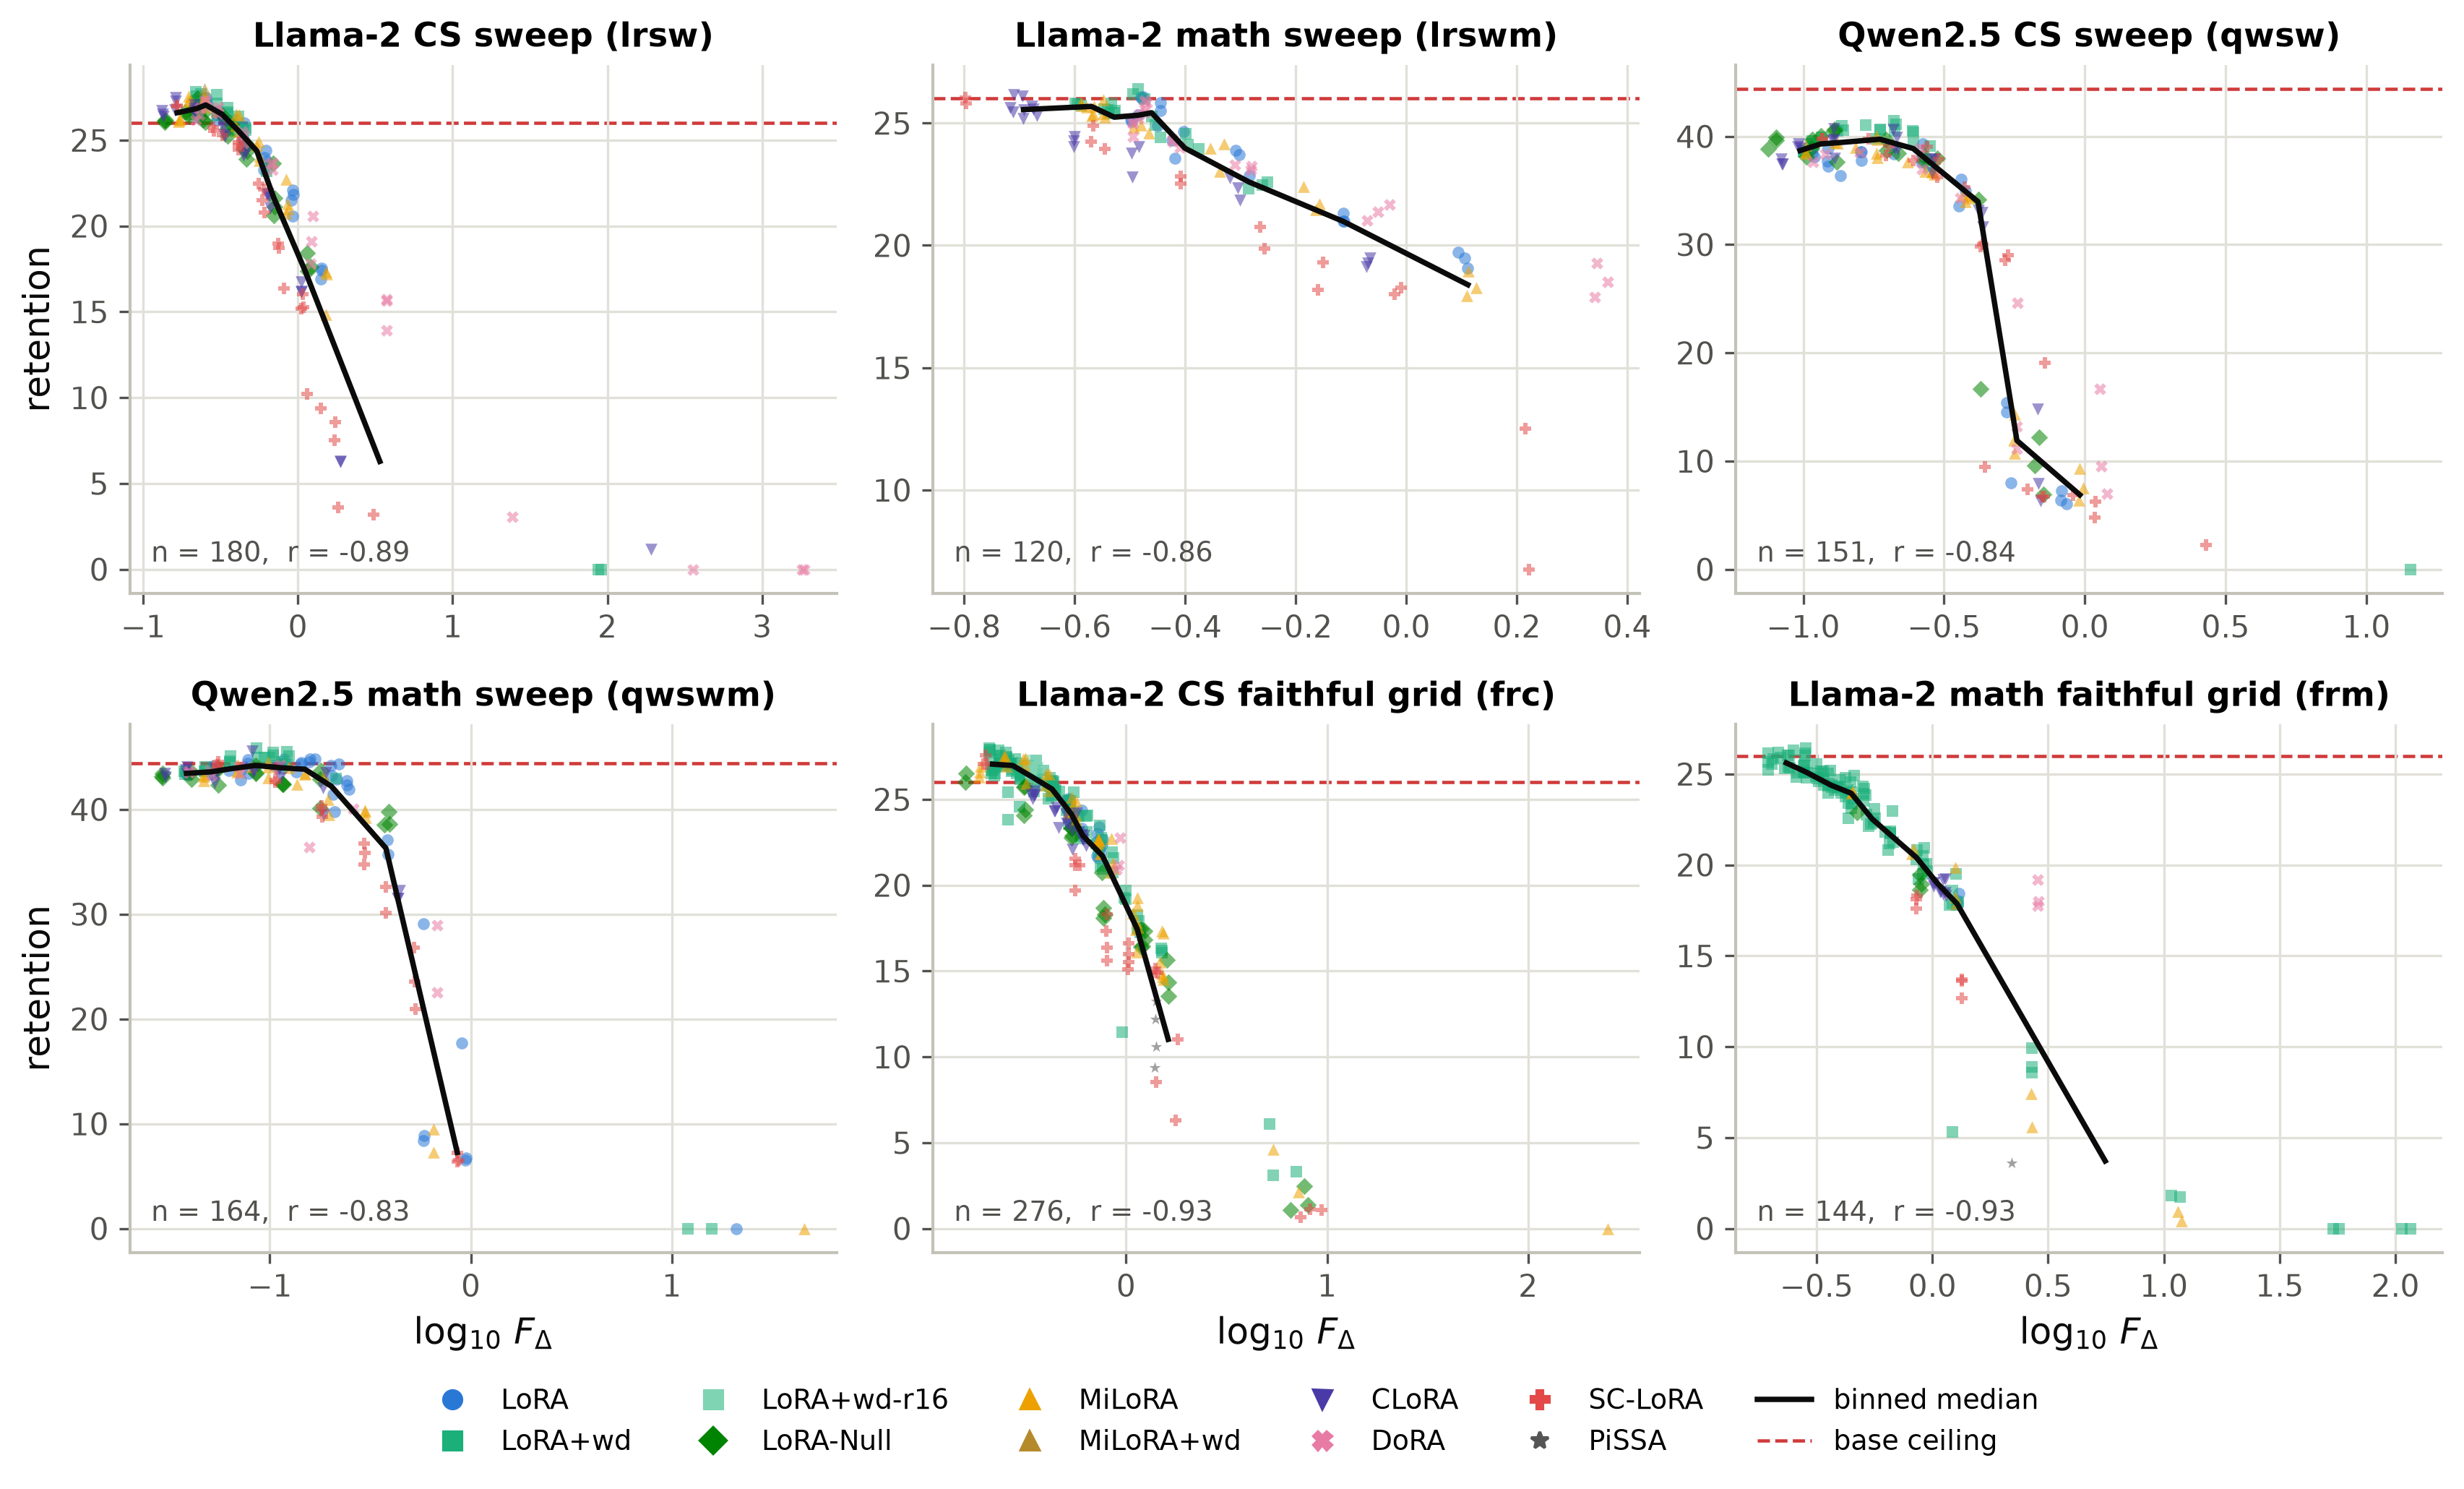
\includegraphics[width=\textwidth]{fig_family_scatter.png}
\caption{Retention against update magnitude $\dw$ (log scale), one panel per
run family, every on-pool run shown as one point colored by method. The solid
line is the binned median; the dashed line is the base model's core
retention (the correlational pool scores every family, math included, on core
retention; the metric definitions are in Section~\ref{sec:method:metrics}). In
every family the runs of all methods interleave along a single flat-then-falling
trend: retention holds near the base ceiling while updates stay small and
falls once they grow past the knee. The correlation between log update
magnitude and retention is strongly negative in all six families, ranging
from $r=-0.83$ to $r=-0.93$
(lrsw $r=-0.886$, $n=180$; lrswm $r=-0.865$, $n=120$;
qwsw $r=-0.840$, $n=151$; qwswm $r=-0.830$, $n=164$, or $-0.695$ on its
format-collapse-clean subset, $n=155$;
frc $r=-0.928$, $n=276$; frm $r=-0.929$, $n=144$).}
\label{fig:family-scatter}
\end{figure*}

\paragraph{The rescaling intervention (Section~\ref{sec:results:rq2}).}
Rescaling a trained adapter's update by a constant changes its magnitude and
nothing else. The $15$ trained rescales land at a mean residual of
$+1.29\!\pm\!2.07$ points from the family curve, and the nine
random-direction controls at the same magnitudes land at $-1.76\!\pm\!1.32$,
so the direction penalty is the $3.05$-point difference between them. The
intervention ran on Llama commonsense only.

\paragraph{The relation inside a single learning rate
(Section~\ref{sec:results:rq2}).} Among runs sharing one learning rate, the
correlation between magnitude and retention is $-0.7$ or stronger at every
rate of $10^{-4}$ and above; below that rate the curve is flat, so there is
little for the correlation to pick up.

\paragraph{The single-rate comparison artifact
(Section~\ref{sec:results:rq2}).} Because the same learning rate produces a
different update size for each method, the winner of a comparison at one
shared rate is partly decided by which method that rate happens to suit. Our
grid shows the size of the effect: of the five adapters that modify LoRA's
structure (CLoRA, MiLoRA, SC-LoRA, LoRA-Null, DoRA), four beat plain LoRA at
their own best single rate on a single seed, by up to $+26$ adaptation
points (Figure~\ref{fig:lrartifact}, Table~\ref{tab:lr_artifact}), yet once
every method is swept over rates, the LoRA{+}wd frontier sits on or above
all of them. Per-adapter sweeps are in Appendix~\ref{app:lrsweep}.

\paragraph{The safe learning-rate band
(Section~\ref{sec:results:rq2}).} One rate counts as safe for one method when
that method's cell mean retention at that rate stays within $2$ points of its
base model's retention. Only rates up to $10^{-3}$ are counted, since the two
higher rates were attempted on Llama commonsense only and mostly diverged there
(Appendix~\ref{app:sweep}). Counted this
way, LoRA{+}wd is safe at $26$ of its $29$ rate-by-setting cells and SC-LoRA at
$6$ of its $25$. The denominators differ because per-method rate coverage
differs in the Llama math grid, where LoRA{+}wd was run at six rates and
SC-LoRA at two; the other three settings offer both arms the same rates.
Qwen commonsense is the one family scored against
the best retention observed inside the family rather than against the base
model, because on that setting no method stays within $2$ points of the Qwen
base at any rate: commonsense tuning costs every adapter at least a few points
of core retention there, which is a fact about the family and not a ranking of
methods. That family-best reference, $41.03$, is itself a single-seed
off-grid cell, so the Qwen commonsense counts are the softest part of this
tally. The per-method curves are Figure~\ref{fig:lrband}.

\paragraph{The adaptation side of the same relation
(Section~\ref{sec:results:rq2}).} A flat-then-falling fit
explains $0.78$ to $0.88$ of retention variance within family but only $0.26$
to $0.66$ of adaptation variance in five of the six families (a quadratic fit
gives $0.71$ to $0.87$ and $0.19$ to $0.66$), so adaptation is
the axis on which methods can still differ, and the one suggestive gain of
Section~\ref{sec:results:rq1} is an adaptation gain. Larger updates do not buy
more adaptation either. Adaptation is concave in update magnitude, with a
negative quadratic term required in all six families (cluster-robust $t$
between $-3.1$ and $-17.9$): it rises only up to an optimum band and falls at
$20$ to $37$ points per decade beyond it, and that band sits at the retention
knee in five of the six families. Forgetting beyond the knee is therefore a
pure loss rather than a price paid for a better-adapted model.

\paragraph{How the retention variance splits between magnitude and geometry
(Section~\ref{sec:results:rq2}).} The nested ladder of
Table~\ref{tab:ladder} adds blocks in one fixed order. The order-free
commonality split removes that dependence: it attributes $+0.296$ of
retention variance ($95\%$ confidence interval $[+0.203, +0.386]$) uniquely to
magnitude, $+0.016$ ($[+0.006, +0.032]$) uniquely to shape-only geometry, and
$+0.099$ to the two blocks jointly. This paper uses two different geometry
blocks and each result names the one it uses: the shape-only block here is
$e_{\mathrm{top}}$ together with stable rank, and it leaves out the spectral
norm, which is itself a size measure; the ladder of Table~\ref{tab:ladder} uses
the wider block that includes the spectral norm. Measuring the placement
construct of Section~\ref{sec:related} on its own terms gives a smaller
step, not a larger one: with the block reduced to the four energy shares, so
that placement is separated from shape and size, geometry adds $+0.008$, and
adding the two input-side shares to the ladder's block leaves it at
$+0.017$. Read as single predictors over family fixed effects, stable rank
reaches $\Delta R^2 = 0.116$ against magnitude's $0.420$ ($n = 911$), a
factor of about $3.6$ rather than $23$ (per-metric ranking in
Table~\ref{tab:league}).

\paragraph{The weaker accounting, disclosed
(Section~\ref{sec:results:rq2}).} Adding KL drift as a third predictor block
(common sample $n\!=\!911$) shrinks every unique share, because the three
blocks overlap heavily: magnitude falls to $+0.033$, the five-metric shape
block to $+0.031$, and drift to $+0.009$, and magnitude's unique share then
exceeds both of the others in only $1{,}078$ of $2{,}000$ bootstrap
replicates, little better than chance. We read that as overlap rather than as
weakness, because drift and magnitude track the same forgetting: taken two
blocks at a time on the same sample, drift adds only $+0.005$ of retention
variance beyond magnitude while magnitude adds $+0.085$ beyond drift, with
$+0.335$ shared between them (single-predictor ranking:
Table~\ref{tab:league}; monitor results: Section~\ref{sec:results:rq3}).

\paragraph{The residual geometry effect
(Section~\ref{sec:results:rq2}).} Once magnitude is known, the leverage left
to update shape is the partial correlation $r(\text{stable rank},
\text{retention} \mid \log\dw)$, which runs from $-0.32$ to $-0.67$ on the
four Llama families and is near zero on the two Qwen families, so the residual
effect is real but model-dependent. Per family it is $-0.595$ on Llama
commonsense ($n\!=\!180$), $-0.666$ on Llama math ($n\!=\!120$), $-0.333$
and $-0.323$ on the two denser Llama grids ($n\!=\!275$, $144$), and
$-0.004$ and $+0.073$ on Qwen commonsense and Qwen math ($n\!=\!151$,
$164$). Fitting retention on $\log\dw$ and method dummies within a family
puts the per-method offsets at up to about five points, largest for SC-LoRA on
Llama and not significant on either Qwen family; the SC-LoRA offset tracks
the calibration corpus rather than the subspace constraint, as the
eval-matched calibration control shows (Appendix~\ref{app:sweep}). In the ladder
of Table~\ref{tab:ladder} the standardized coefficient on $\log\dw$ is
$-0.744$ $[-0.894, -0.615]$ against $|\beta|\!\le\!0.138$ for every
geometry measure, with cluster-robust $t(\log\dw)\!=\!-7.9$.

\paragraph{What the geometry ceiling does and does not bound
(Section~\ref{sec:results:rq2}).} The ceiling bounds geometry effects that
separate one design from another, since a feature constant within a method
lies in the span of the method dummies and method identity adds $+0.016$
over size alone. It does not bound an effect that varies from run to run
inside a method, and the knobs that would generate the intruder directions
of \citet{shuttleworth2025illusion}, rank, scaling factor and learning rate,
vary that way in our pool. Nor does the small step contradict the
$3.05$-point random-direction penalty of the rescaling intervention above: a
random subspace takes about its dimensional share of energy at either end of
the spectrum, which is an ordinary placement, so the penalty the control
detects is a direction effect that placement does not carry, and the ceiling
bounds placement, not direction in general. Everything here is computed on
$\Delta W$ and never on the adapted matrix $W_0{+}\Delta W$, where they
locate their effect (coordinates and blocks in Appendix~\ref{app:geoproj}).

\begin{figure*}[t]
\centering
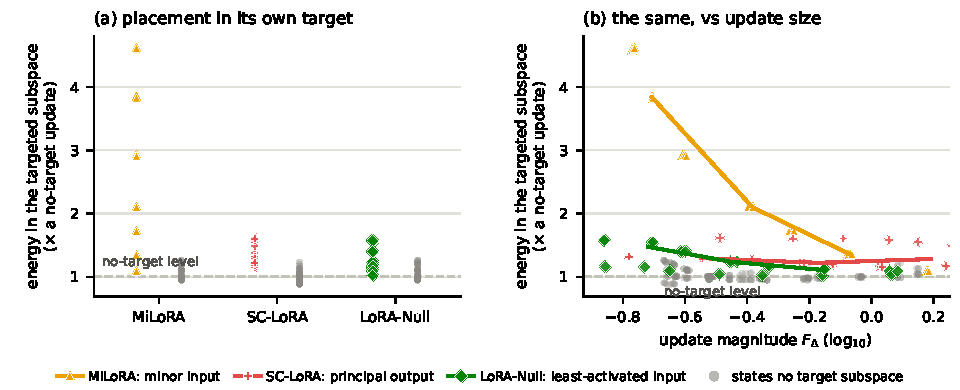
\includegraphics[width=\textwidth]{fig_geometry.pdf}
\caption{Whether each design places its update in the subspace its own
initialization targets, on the Llama-2-7B commonsense sweep, every run
shown. (a) The energy each design puts in the subspace it targets, as a
multiple of what a method that targets nothing puts there, so one means no
difference. (b) The same quantity against update magnitude, where MiLoRA's
placement falls back toward the reference as updates grow and SC-LoRA's
does not vary.}
\label{fig:placement}
\end{figure*}

\paragraph{The placement each design makes, across run families
(Section~\ref{sec:results:rq2}).} Figure~\ref{fig:geometry} shows that
each design leaves a distinctive trace; the stricter question is whether
that trace lies in the subspace the design's own paper states, which
Figure~\ref{fig:placement} answers on the
Llama-2-7B commonsense sweep. Each design is scored on the base-weight
subspace its own initialization targets, which we read from the
initialization code rather than from the descriptive text: MiLoRA the
minor input directions, LoRA-Null the least-activated input directions,
and SC-LoRA the principal output directions, since SC-LoRA sets its
up-projection from the top eigenvectors of the output second moment and
its much larger share in the principal input directions follows from that
construction rather than from a stated target. Taking each method's own
target column and comparing the median over the smallest third of its runs
by update magnitude against the median over the largest third, the ratio
of large to small is $0.31$ to $0.47$ for MiLoRA over all six run families
and $0.53$ to $0.83$ for LoRA-Null over four; the correlation between the
placement and $\log_{10}\dw$ within a family runs from $-0.81$ to $-0.98$
for MiLoRA and from $-0.66$ to $-0.99$ for LoRA-Null. SC-LoRA shows no
such relation on its own target: the ratio is $0.92$ to $1.15$ over five
families and the correlation has no consistent sign, from $-0.63$ to
$+0.90$. Its placement is also the smallest of the three, $1.05$ to $1.51$
times the no-target level on Llama and $0.91$ times on Qwen commonsense,
which is at that level rather than above it. We report a family only where
the method has at least ten runs in it, which excludes the Llama math grid
for SC-LoRA and LoRA-Null. PiSSA runs only at its recipe rate and so spans
no magnitude range, and it is not part of this comparison. Two controls: the energy shares and the
stable rank are unchanged if the update is multiplied by a constant, so
none of these quantities can track the update's size by construction, and
over the same magnitude range the methods that state no target subspace
stay flat on the same columns, which rules out the reading that any large
update loses share in any fixed subspace. Within a sweep the update
magnitude and the learning rate move together, so we describe the relation
on the magnitude axis that was swept and do not separate the two.
Finally, one disclosure: in the two commonsense sweeps SC-LoRA's seed-$42$
runs sit at roughly twice the update magnitude of its seeds $43$ to $45$
at every learning rate, while those three agree to three decimals with
each other, which is a larger gap than seed variation produces elsewhere
in the pool. Those runs are retained in Figure~\ref{fig:placement} and in
every statistic above; they are the widest points in the SC-LoRA column. On the $49$-cell single-seed Llama
commonsense subset, allowing each method its own slope on top of its own
intercept leaves the six on-curve series statistically indistinguishable
($F(5,30)\!=\!0.28$, $p\!=\!0.92$). Over all seven series the same tests are
significant, $F(6,41)\!=\!7.05$ for the intercepts and $F(6,35)\!=\!9.32$ for
the slopes, both $p<0.001$, and both are driven almost entirely by SC-LoRA.
Holding one method out at a time, a pooled
fit that has never seen it predicts its retention at a mean root-mean-square
error of $2.5$ points, against $2.2$ for the method-aware in-sample fit.
Held-out SC-LoRA is the exception, missing by $9.1$ points, which is the
calibration-corpus effect the eval-matched control isolates
(Appendix~\ref{app:sweep}). The full geometry
battery per method and base model, with each design's advertised subspace
marked, is Table~\ref{tab:geometry-battery}.

% AUTO-GENERATED by acl_analysis/observatory/37_geometry_battery_table.py
% from m3_master.csv (on-pool; 30_m3_geometry.py run-level pooling) joined
% with acl_analysis/insights/pool.csv for the input-side energies, and
% cross-checked against analysis_final/dyn4_geometry.txt G1 (which pooled
% over swept cells; its LoRA/LoRA+wd stable-rank medians differ by 0.5-1.9,
% all energies agree within 0.02). The generator aborts on any drift from
% its frozen anchors. Do not hand-edit; rerun the script.
% Needs \usepackage{colortbl} (xcolor already in the preamble); geoblue
% is also defined by tables/table_geometry_fingerprint.tex.
\providecolor{geoblue}{RGB}{0,114,178}
\begin{table*}[t]
\centering
\footnotesize
\setlength{\tabcolsep}{5pt}
\renewcommand{\arraystretch}{1.12}
\begin{tabular}{l rrrrr rrrrr}
\toprule
 & \multicolumn{5}{c}{Llama-2-7B} & \multicolumn{5}{c}{Qwen2.5-7B} \\
\cmidrule(lr){2-6} \cmidrule(lr){7-11}
 & & & \multicolumn{3}{c}{share of update energy in} & & & \multicolumn{3}{c}{share of update energy in} \\
 & & & \multicolumn{3}{c}{base directions} & & & \multicolumn{3}{c}{base directions} \\
\cmidrule(lr){4-6} \cmidrule(lr){9-11}
Method & $n$ & SR & top out & top in & bottom in & $n$ & SR & top out & top in & bottom in \\
\midrule
\multicolumn{11}{l}{\emph{states no target subspace (LoRA row is the reference for every column)}} \\
LoRA & 65 & 4.6 & 0.068 & 0.075 & 0.050 & 69 & 6.3 & 0.114 & 0.067 & 0.049 \\
LoRA{+}wd & 274 & 9.9 & 0.073 & 0.085 & 0.049 & 47 & 6.8 & 0.116 & 0.075 & 0.047 \\
DoRA & 52 & 3.5 & 0.070 & 0.089 & 0.050 & 24 & 5.1 & 0.115 & 0.071 & 0.049 \\
CLoRA & 79 & 7.6 & 0.061 & 0.067 & 0.050 & 43 & 8.6 & 0.054 & 0.060 & 0.047 \\
\midrule
\multicolumn{11}{l}{\emph{states a target subspace (marked cell is the closest proxy in this basis)}} \\
MiLoRA & 109 & 5.9 & 0.067 & 0.073 & \cellcolor{geoblue!42}0.092 & 48 & 10.7 & 0.069 & 0.061 & \cellcolor{geoblue!42}0.214 \\
LoRA-Null & 55 & 8.8 & 0.104 & 0.104 & \cellcolor{geoblue!12}0.059 & 41 & 7.9 & 0.176 & 0.081 & \cellcolor{geoblue!14}0.105 \\
SC-LoRA & 69 & 14.2 & \cellcolor{geoblue!12}0.086 & 0.317 & 0.020 & 43 & 15.3 & \cellcolor{geoblue!22}0.147 & 0.247 & 0.028 \\
PiSSA & 5 & 18.0 & \cellcolor{geoblue!42}0.221 & \cellcolor{geoblue!42}0.457 & 0.028 & -- & -- & -- & -- & -- \\
\bottomrule
\end{tabular}
\caption{Update geometry per method and base model: run-level
medians over the on-pool 7B runs, with plain LoRA as the reference row
for every column and the number of runs per block. Each energy column
is the share of the update's energy in a fixed $256$ base-weight
singular directions (top output, top input, bottom input); the neutral
level differs by column and model (Qwen's attention k/v matrices have
only $512$ output directions), so values read against the column's
LoRA reference, not across columns. The marked cell in each row is the
closest proxy in this basis for the target the method's own paper
states, and it sits above the LoRA reference in every case; SC-LoRA's
large top-input share is an initialization side effect, and CLoRA
penalizes a random per-module subspace this basis does not measure. SR
is the stable rank of the update; the stable-rank split recurs at 284B
(Table~\ref{tab:ds284b}); PiSSA has no Qwen-2.5 arm.}
\label{tab:geometry-battery}
\end{table*}


\paragraph{Adaptation and retention over the whole pool
(Section~\ref{sec:results:rq2}).} Pooled over the frozen pool the two axes are
positively rather than negatively associated, because runs at excessive update
magnitude lose both at once. The association weakens when the quarantined
collapse runs are excluded, so a genuine trade-off appears only near each
recipe's own frontier.

\paragraph{The drift monitor (Section~\ref{sec:results:rq3}).} The Llama
prediction error of $1.3$ to $2.0$ points compares against a seed-noise floor
of $0.4$ to $0.9$ points on the same cells. Counting a run as damaged when it
falls more than $5$ points below the best retention in its own run family,
drift separates damaged from healthy runs at an area under the curve (AUC) of
$0.976$ to $0.996$ in all six families, the AUC being the probability that a
damaged run shows higher drift than a healthy one. Damage sets in near $0.26$
to $0.30$ nats of drift, a nat being the natural-logarithm unit of KL
divergence, in four of the six families. Where adapter weights are available,
$\log\dw$ separates damaged from healthy runs at an AUC of $0.98$ to $1.00$.
On Qwen the mapping error is driven by a few extreme runs. Two qualifications
apply throughout: drift is a consequence of the update rather than a knob that
sets it, and it is blind to answer-format collapse, where the model still
knows the content but stops producing an answer the parser can extract (the
$\dagger$ cases of Table~\ref{tab:grand-full}).

\paragraph{Predicting seed instability (Section~\ref{sec:results:rq3}).} Call
a cell unstable when its retention varies across its seeds by more than $3$
points of standard deviation, so that re-running the same configuration with a
new seed is a gamble. Whether a train-time signal can identify the unstable
cells among the $290$ multi-seed cells in advance is scored by the AUC: rank
all cells by the signal, and the AUC is the probability that a randomly
chosen unstable cell ranks above a randomly chosen stable one, where $0.5$ is
chance and $1$ is perfect separation. A cell's mean $\log\dw$ reaches AUC
$0.80$; on Llama, the spread of KL drift within a cell reaches AUC $0.96$.
Both signals are available before any benchmark is run. Unstable cells sit a
median of $0.49$ decades of $\dw$ above their family knee, against $0.02$
decades for stable cells (Mann-Whitney $p\!=\!2\times10^{-6}$).

\paragraph{Benchmark fragility (Section~\ref{sec:results:rq4}).}
TruthfulQA's cell-level correlation with forgetting is $+0.40$ to $+0.79$ on
the four Llama families and $-0.87$ and $-0.90$ on the two Qwen families.
Part of the fragility order could reflect distance to the chance floor, since
MMLU-Pro is 10-way. Including the contaminated ARC-Challenge in the ranking
gives Kendall's $W\!=\!0.906$ instead of $1.000$; including TruthfulQA in the
broad retention aggregate, which is the mean over all the general benchmarks,
makes that aggregate's slope shallower by $24$ to $30\%$ on Llama.

\paragraph{At matched update magnitude, method differences concentrate in
MMLU-Pro.} At matched update magnitude, method identity leaves BBH nearly
unchanged but separates on MMLU-Pro: relative to LoRA{+}wd, the remaining
methods lose more MMLU-Pro than BBH in $31$ of $37$ magnitude-matched
method-family combinations (raw points; Wilcoxon $p<0.01$ for SC-LoRA,
LoRA-Null, and CLoRA), with excesses of up to about $3$ points. Where
methods differ at all at matched update magnitude, they differ on the most
fragile, format-following benchmark rather than uniformly across the suite.

\paragraph{Knob effects on the retention-magnitude slope, and the SC-LoRA
exception.} Within family, the
retention-magnitude slope is statistically indistinguishable across weight
decay and across the geometry-constrained versus plain method class
(interaction $|t| \le 1.64$, cluster-robust; the weight-decay interaction is
$+11.1$ against a main slope of $-16.2$, with a cell-bootstrap $95\%$
confidence interval of $[-15.4, +40.1]$), which is consistent with those two
knobs moving a recipe along the magnitude curve rather than changing its slope.
The rank interaction points the same way but carries almost no information:
$t\!=\!+1.69$ with a cell-bootstrap interval of $[-16.0, +1383.6]$, estimated
from only seven runs at ranks $8$ and $16$. We read it as a null result, not as
evidence that rank leaves the slope alone. The one repeatable exception is
SC-LoRA, which falls progressively further below the family curve as magnitude
grows: it has the steepest per-method slope in all five estimable families,
its slope excess over LoRA{+}wd is significant in two of them, and part of its
Qwen component is carried by quarantined collapse runs. Because the
eval-matched calibration control removed SC-LoRA's retention offset on Llama
commonsense, we attribute the excess slope to the method as configured rather
than to its subspace constraint.

% NEW (round-5, ACL repositioning). League table for the Four-Instruments
% section: which single metric predicts retention. Source:
% acl_analysis/correlations/{findings.md section 2, 03_league_table.py,
% league_table.md}; all cells CONFIRMED exactly by the independent verification
% pass (verification_report.md B4 -- reproduced to the value and the cluster-t).
% Same-sample n=911 (CE-and-geometry pool), delta-R^2 over family fixed effects,
% cluster-robust (cluster = recipe cell) per 09 Q1. spec_max is listed under
% MAGNITUDE (r=+0.93 with log F_Delta family-demeaned; 06 section 5, 09 Q1c).
% \footnotesize + tightened headers to clear a prior 21pt overfull hbox.
\begin{table}[t]
\centering
\footnotesize
\setlength{\tabcolsep}{4pt}
\caption{\textbf{The four instruments, ranked as single predictors of
retention.} Same-sample $\Delta R^2$ over family fixed effects
($n\!=\!911$, cluster-robust). The three magnitude measures top the table;
behavioral drift (KL) is a near-substitute but downstream; learning rate is the
fifth of the ten ranked metrics; every update-shape geometry metric is last.
$\dw$ is the best single member. Condensed from the ten-metric ranking; the last
row groups the remaining geometry terms.}
\label{tab:league}
\begin{tabular}{l l c c}
\toprule
Metric & Block & $\Delta R^2$ & $R^2$ range \\
\midrule
$\log\dw$              & magnitude  & $+0.420$ & 0.69--0.86 \\
$\log\smax$            & magnitude  & $+0.349$ & 0.57--0.75 \\
$\log\lVert\Delta W\rVert_F$ & magnitude & $+0.348$ & 0.50--0.83 \\
KL drift (CE)          & behavioral & $+0.340$ & 0.41--0.86 \\
$\log(\text{LR})$      & training   & $+0.207$ & 0.22--0.52 \\
stable rank            & geometry   & $+0.116$ & 0.08--0.67 \\
amp$_{\rm top}$/$e_{\rm top}$ & geometry & $\le\!+0.032$ & 0.00--0.24 \\
\bottomrule
\end{tabular}
\end{table}


% AUTO-GENERATED by make_table_lr_artifact.py (_paper mode) -- do not hand-edit.
% PAPER-LOCAL variant of table_lr_artifact.tex: same numbers (dedup by latest
% evaluated_at, Llama-2 CS, seed 42, 7 LRs), CorDA row removed (embargoed), and
% the PI-edited 'ingredients' caption reproduced verbatim as a literal.
\begin{table*}[t]
\centering
\small
\setlength{\tabcolsep}{4pt}
\caption{\textbf{The single-rate advantage of four of the five structure-modifying adapters
carries the ingredients of a learning-rate artifact.} For each method we take its
best-looking single learning rate, the rate with the highest commonsense
adaptation among those keeping retention $\ge 24$. At that fixed rate the method
can beat plain LoRA run at the same rate (columns 2--4). Once the learning rate
is swept, LoRA+wd traces a retention-adaptation frontier that sits on or above
the method's best single-rate point on both axes
(columns 5--6). \emph{Single seed (42); the retention margins are sub-1\,pp and within
documented seed noise; the point is that no fixed-rate advantage survives a symmetric
sweep, not the size of the gap.} Adapt = commonsense accuracy; Ret = mean(BBH,
MMLU-Pro). Llama-2-7B, 7 LRs. CorDA is withheld (see Limitations).
$^{\dagger}$$79.9$ is MiLoRA's \emph{seed-42} best-adapt cell (lr$3\!\times\!10^{-4}$);
across seeds that cell is a format-collapse basin ($79.9/58.7/34.5$, i.e.\
$57.7\!\pm\!22.7$), so the multi-seed exhibit (Table~\ref{tab:grand}) selects a
different, lower best-adapt mean ($77.2$). Retention stays curve-consistent
throughout.}
\label{tab:lr_artifact}
\begin{tabular}{l cc c cc}
\toprule
 & \multicolumn{3}{c}{\textbf{Single-LR view (fixed LR)}} & \multicolumn{2}{c}{\textbf{Swept view}} \\
\cmidrule(lr){2-4}\cmidrule(lr){5-6}
Method & Method @ LR$^\star$ & LoRA @ same LR & $\Delta$adapt & LoRA+wd frontier pt & On/above? \\
 & (adapt / ret) & (adapt / ret) & (pp) & (LR: adapt / ret) & \\
\midrule
DoRA & 78.3 / 24.8 ($2\!\times\!10^{-4}$) & 72.3 / 25.2 & +5.9 & $5\!\times\!10^{-4}$: 81.6 / 25.6 & \textbf{yes} \\
MiLoRA & 79.9$^{\dagger}$ / 24.7 ($3\!\times\!10^{-4}$) & 79.1 / 24.4 & +0.8 & $5\!\times\!10^{-4}$: 81.6 / 25.6 & \textbf{yes} \\
SC-LoRA & 79.5 / 25.3 ($2\!\times\!10^{-5}$) & 53.6 / 26.3 & +26.0 & $5\!\times\!10^{-4}$: 81.6 / 25.6 & \textbf{yes} \\
LoRA-Null & 73.0 / 26.2 ($2\!\times\!10^{-5}$) & 53.6 / 26.3 & +19.5 & $3\!\times\!10^{-4}$: 80.6 / 26.2 & \textbf{yes} \\
CLoRA & 64.9 / 24.3 ($3\!\times\!10^{-4}$) & 79.1 / 24.4 & -14.2 & $5\!\times\!10^{-4}$: 81.6 / 25.6 & \textbf{yes} \\
\bottomrule
\end{tabular}
\end{table*}


\begin{figure*}[t]
  \centering
  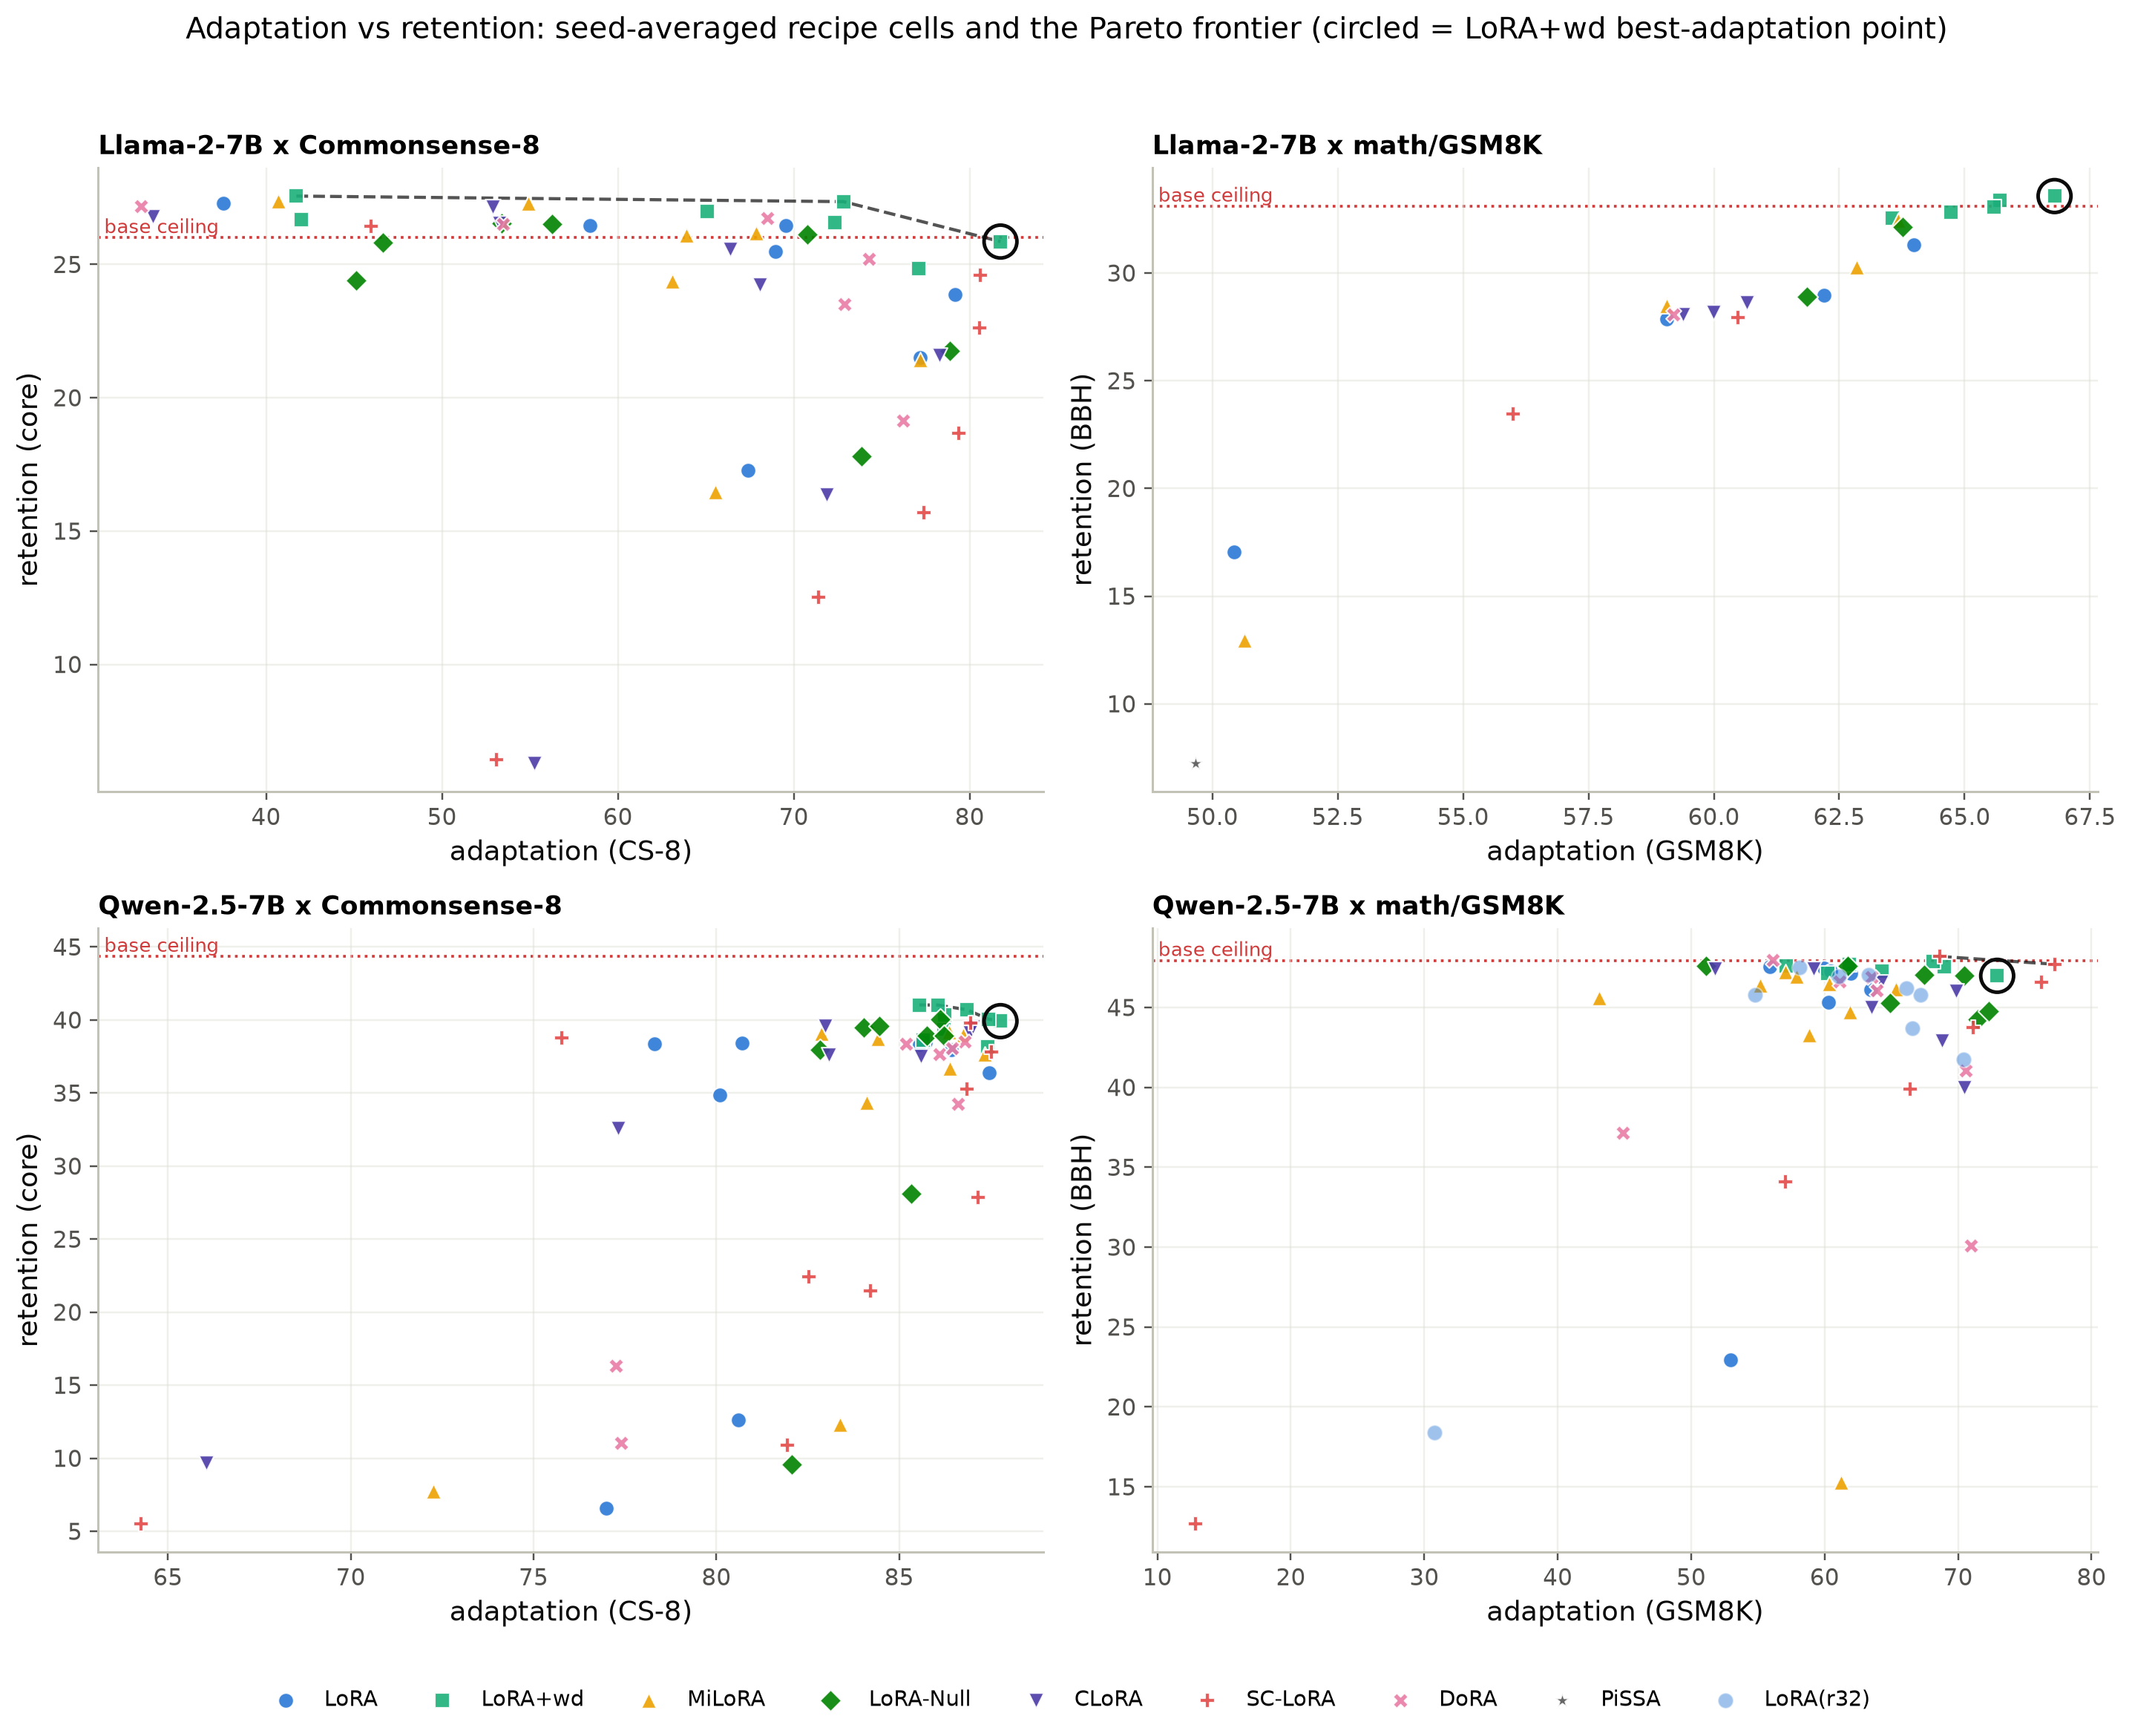
\includegraphics[width=0.92\textwidth]{fig_pareto.png}
  \caption{Adaptation versus retention in the four model $\times$ task
  settings, one point per seed-averaged recipe cell, with the observed
  frontier highlighted; where no frontier line is drawn it consists of a
  single point. LoRA{+}wd is the sole method on the frontier in three of four
  settings, with SC-LoRA on Qwen math the exception; one-cell weight-decay
  transfer arms are excluded from the ranking and CorDA is withheld. Three
  qualifiers on reading it are in Appendix~\ref{app:exhibits}: the frontier
  is a property of the observed points rather than of resampled ones, MiLoRA
  reaches a cell-bootstrap probability of $0.50$ on Llama commonsense, and
  two Qwen commonsense frontier cells are single-seed.}
  \label{fig:pareto}
\end{figure*}

\begin{figure*}[t]
  \centering
  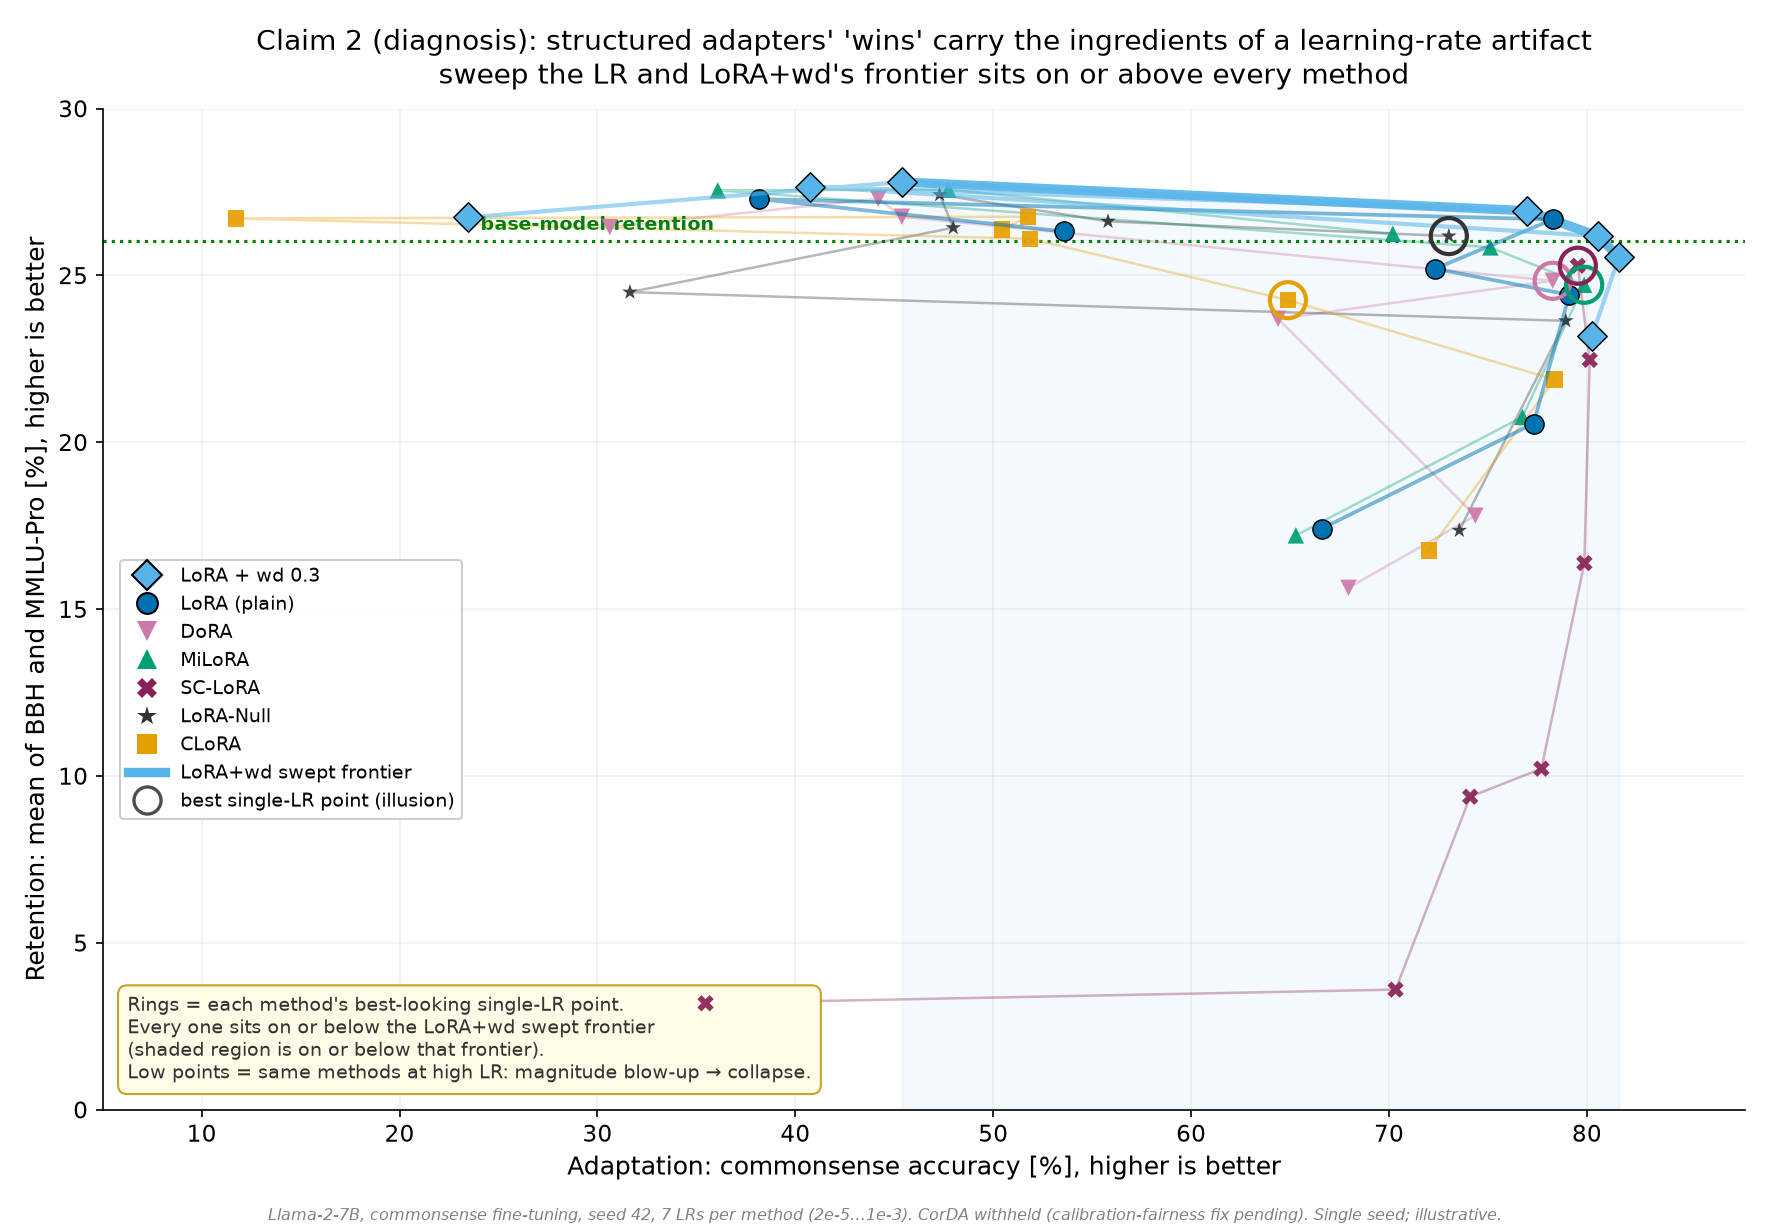
\includegraphics[width=0.8\textwidth]{fig9_lr_artifact.png}
  \caption{Adaptation and retention over the full seven-rate sweep, per method
  (Llama-2-7B commonsense; Section~\ref{sec:results:rq2}). Each trajectory is
  one method across its seven learning rates in the adaptation-retention
  plane. Rings mark each method's best-looking single rate; the shaded region
  is on or below the swept LoRA{+}wd frontier, so a ring inside it marks a
  single-rate point the swept frontier already reaches. At the highest rates
  the data-aware initializations collapse. Numeric detail in
  Table~\ref{tab:lr_artifact}; CorDA withheld.}
  \label{fig:lrartifact}
\end{figure*}

% NEW (round-5, ACL repositioning). The "cost of geometry" overhead table.
% Source: acl_analysis/adjudication/{findings.md, tables/overheads.md, 05_overheads.py}.
% Verification status (verification_report.md): train wall-clock and init-tax are
% [EXTERNAL] measured constants traceable to the pre-existing registry /
% INTERESTING_INSIGHTS.md section 7 / fig_efficiency.py (DoRA 2.15x, CLoRA GB) --
% CONFIRMED-as-sourced (item 3, "analytical, not metered peak" label kept). The
% "Ret @ matched adapt" column is the adjudication verdict layer's LR-re-matching
% interpolation (verifier item 2: NOT independently re-derived, directionally
% consistent with the verified op-point tables) -- caption sources it accordingly.
% CLoRA memory is an ANALYTICAL resident size (frozen-P block), not metered peak.
\begin{table*}[t]
\centering
\small
\setlength{\tabcolsep}{6pt}
\caption{\textbf{The cost of geometry.} Every structure-modifying adapter pays
extra cost relative to LoRA{+}wd for no retention at matched adaptation. Train
wall-clock
(registry medians) and init taxes are measured; CLoRA memory is the analytical
resident size of its frozen block ($k{=}1024$; $6.69$\,GB at $k{=}2048$), not
metered peak. The last column (mean over four families; negative $=$ below the
LoRA{+}wd envelope) is the operating-point retention gap, directionally
consistent with the verified operating-point tables, not independently re-derived.
$^{\ast}$SC-LoRA's Llama deficit tracks its calibration corpus
(Section~\ref{sec:results:rq1}), not its subspace constraint.}
\label{tab:cost}
\begin{tabular}{l c l c c}
\toprule
Method & Train & Initialization tax & Deploy $\Delta$ & Ret @ matched adapt \\
\midrule
\textbf{LoRA{+}wd} & $1.00\times$ & none (AdamW flag) & rank-$r$ & \textit{reference} \\
LoRA        & $1.00\times$ & none & rank-$r$ & $-2.2$\,pp \\
MiLoRA      & $1.00\times$ & $160$ weight SVDs & rank-$2r$ & $-2.8$\,pp \\
LoRA-Null   & $1.00\times$ & $256$ calib.\ forwards $+$ eigh & rank-$r$ & $-3.2$\,pp \\
CLoRA       & $1.17\times$ & $k{\times}d$ eigh $+$ frozen-$P$ ($+3.34$\,GB) & rank-$r$ & $-4.2$\,pp \\
DoRA        & $2.15\times$ & none & rank-$r$ & $-4.2$\,pp \\
SC-LoRA     & $0.99\times$ & $512$ calib.\ forwards $+$ eigh & rank-$r$ & $-4.6$\,pp$^{\ast}$ \\
\bottomrule
\end{tabular}
\end{table*}


\begin{figure*}[t]
  \centering
  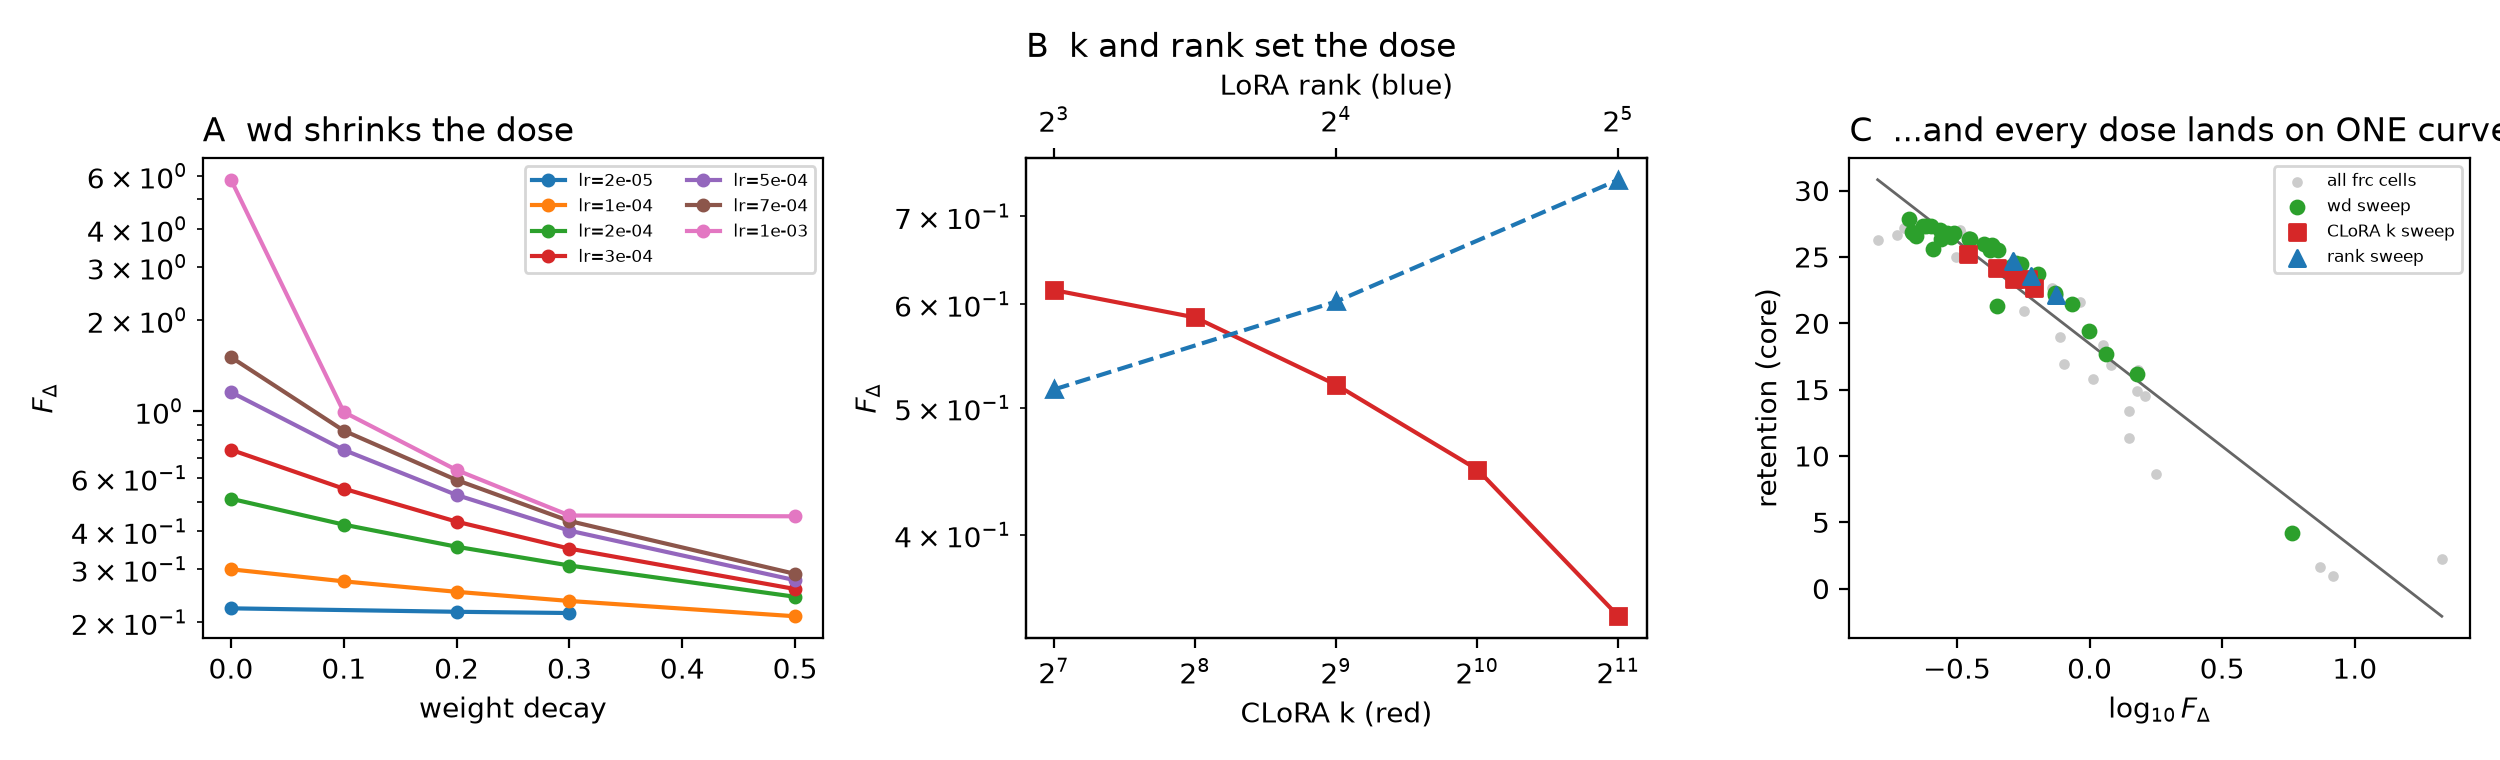
\includegraphics[width=\textwidth]{fig_dose_response.png}
  \caption{Three ways of changing the update magnitude
  (Section~\ref{sec:results:rq2}). Panels (a) and (b) show that weight decay,
  CLoRA's null-space dimension $k$, and LoRA rank each move $\dw$
  monotonically; panel (c) plots retention against $\dw$ for all three, which
  land on one curve per run family. Once $\dw$ is known, which knob produced
  it adds at most $\Delta R^2 = 0.006$ to the retention prediction.}
  \label{fig:dose}
\end{figure*}

\begin{figure*}[t]
  \centering
  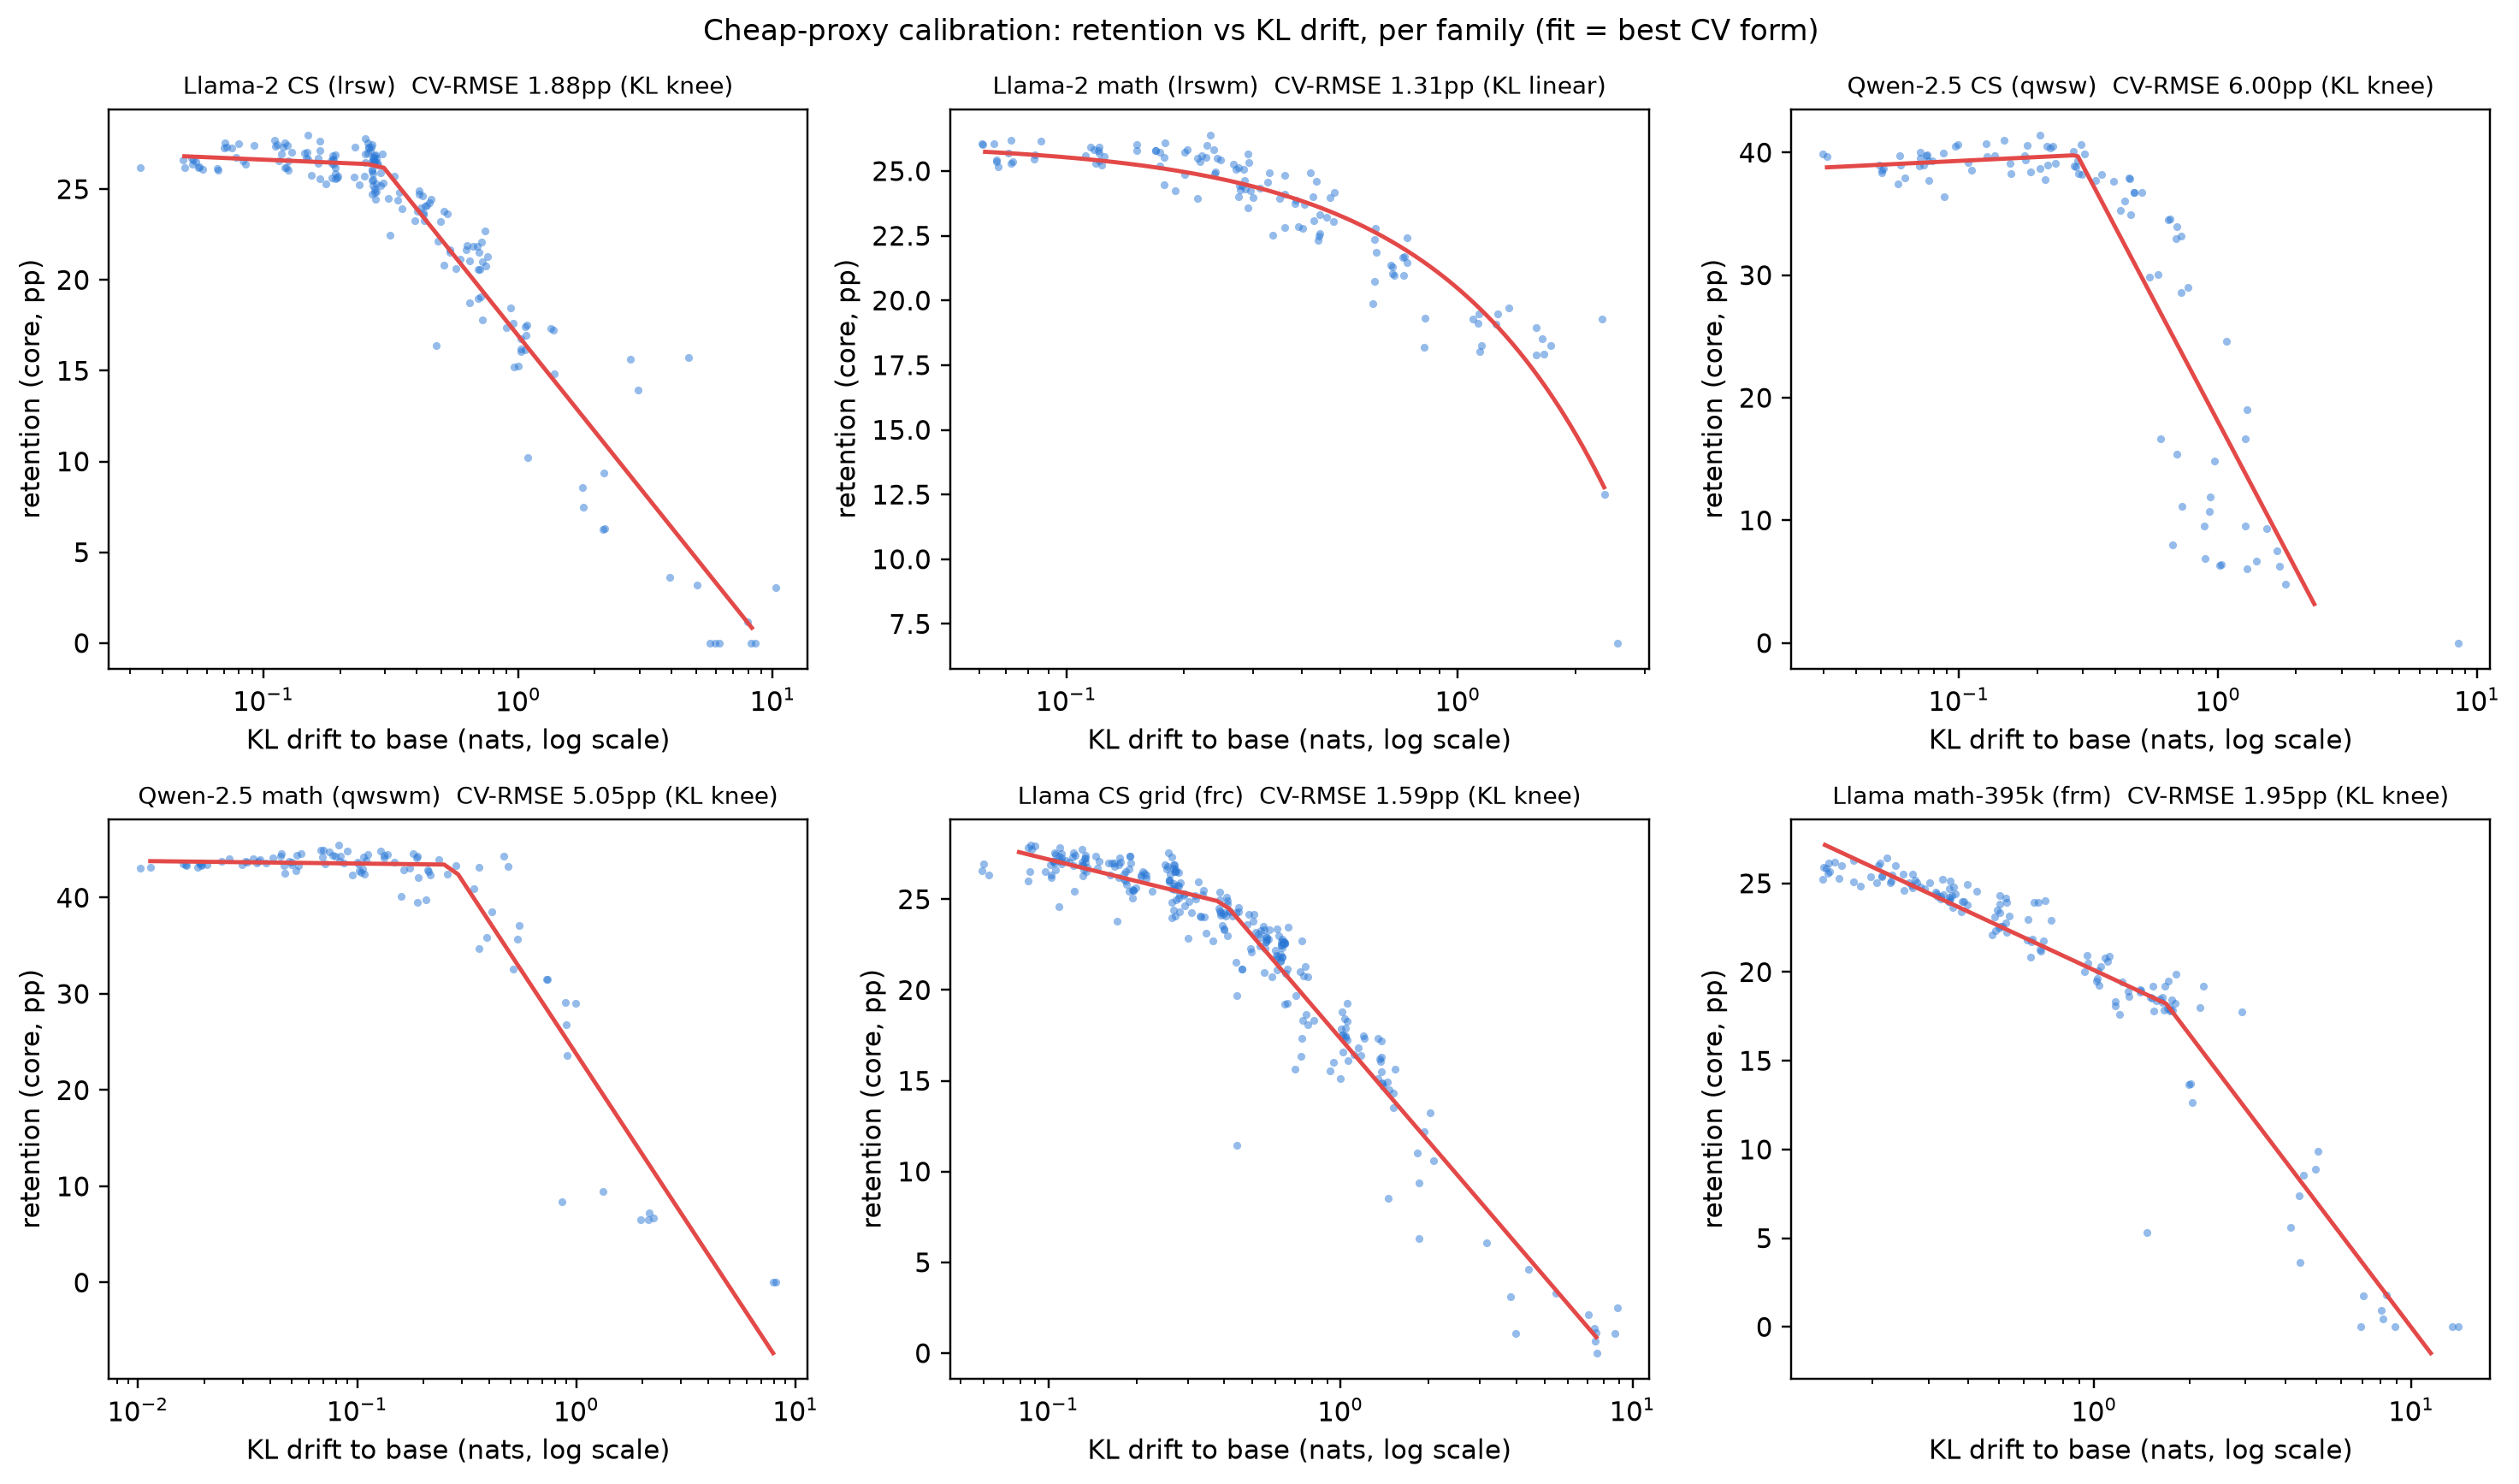
\includegraphics[width=0.92\textwidth]{fig_ce_proxy.png}
  \caption{KL drift as a retention monitor
  (Section~\ref{sec:results:rq3}). Per-family knee-calibrated mapping from
  KL drift to retention; Llama families root-mean-square error (RMSE) $1.3$ to
  $2.0$ points, damage
  AUC $\ge 0.976$, knee near $0.3$ nats. On Qwen the mapping detects
  damage but does not measure it.}
  \label{fig:ceproxy}
\end{figure*}

\begin{figure}[t]
  \centering
  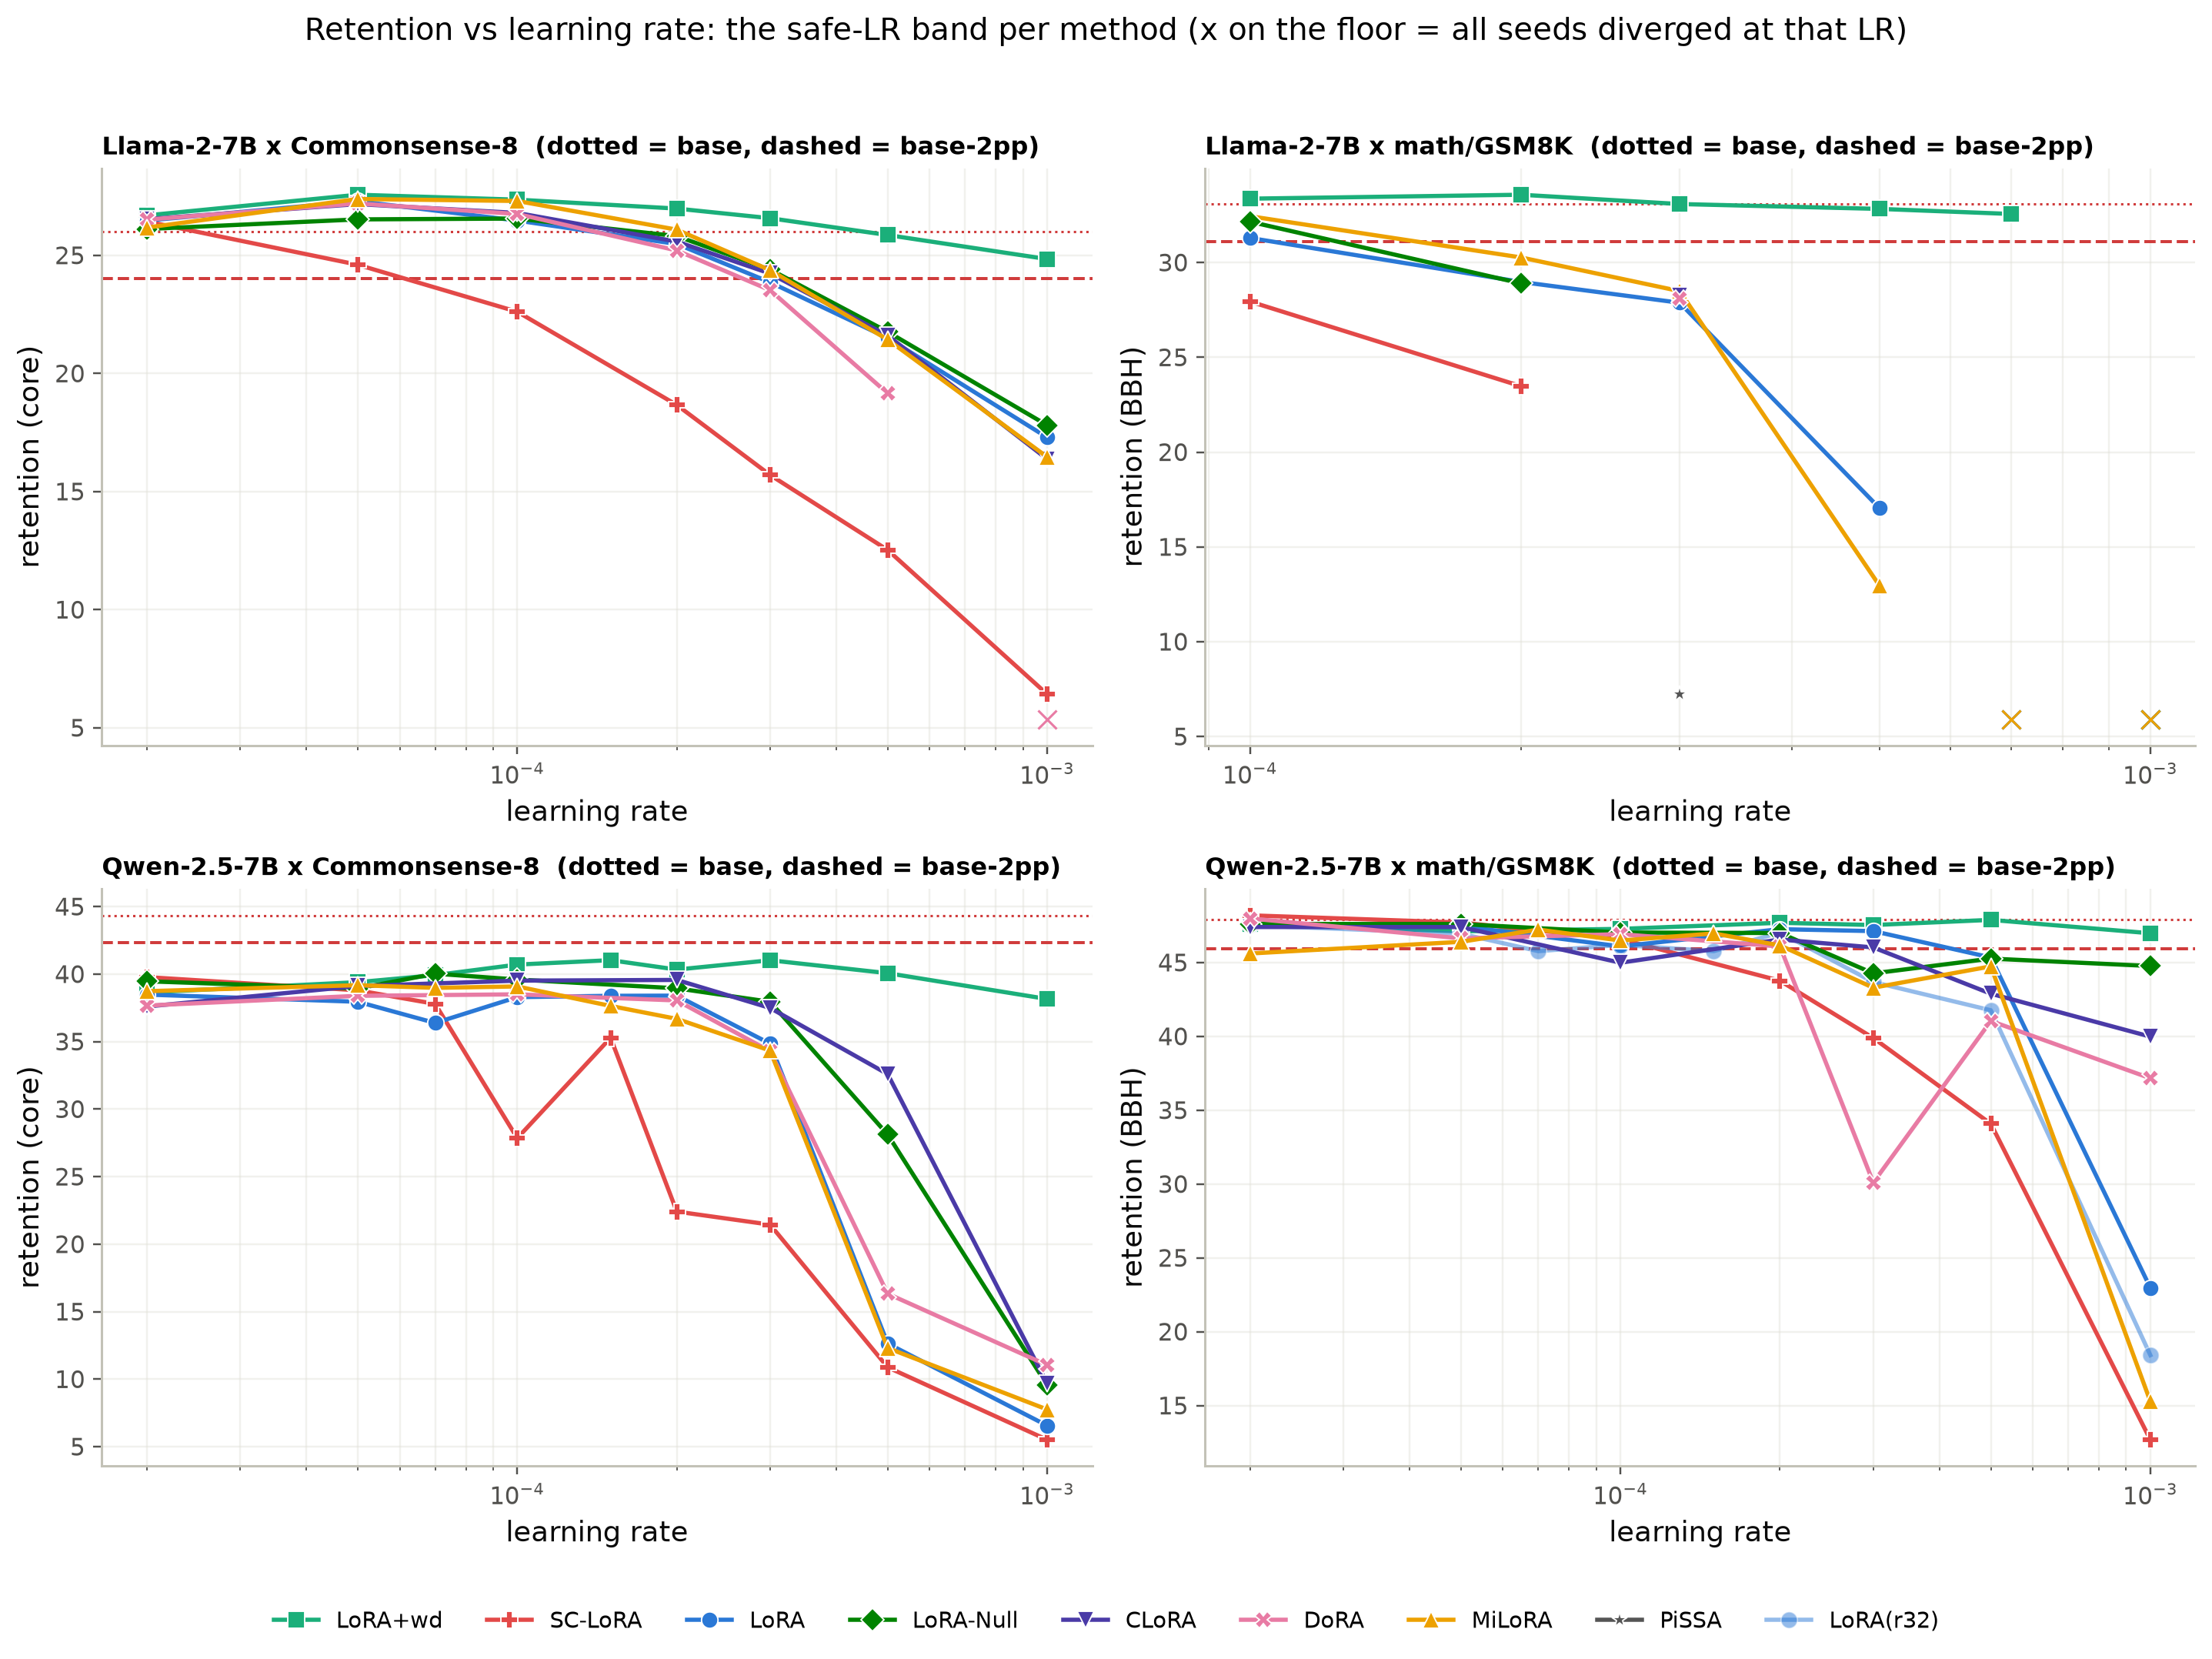
\includegraphics[width=\columnwidth]{fig_lr_band.png}
  \caption{Retention across the learning-rate grid
  (Section~\ref{sec:results:rq2}). At high rates every method other than
  LoRA{+}wd loses retention sharply in some family; LoRA{+}wd stays within
  $2$ points of its reference retention (the base model, and the family best on
  Qwen commonsense) in $26$ of its $29$
  rate-by-setting cells, against $6$ of $25$ for SC-LoRA. The Qwen commonsense
  reference is itself a single-seed cell (text).}
  \label{fig:lrband}
\end{figure}

\begin{table*}[t]
  \centering
  \begin{tabular}{l l c c c}
  \toprule
  Method & Config & GSM8K $\uparrow$ & BBH (retention) $\uparrow$ & $\dw$ $\downarrow$ \\
  \midrule
  \textit{Base (no fine-tuning)} & -- & -- & \textit{33.1} & \textit{0} \\
  \midrule
  LoRA+wd(0.3) & r64, lr 2e-4 & \textbf{67.3} {\footnotesize(3-seed $66.8\pm0.8$)} & \textbf{33.1} {\footnotesize(3-seed $33.6\pm1.0$)} & \textbf{0.28} \\
  LoRA (wd 0)  & r64, lr 1e-4 & 65.0 & 31.0 & 0.43 \\
  MiLoRA       & r64, lr 1e-4 & 62.9 & 32.4 & 0.45 \\
  CLoRA-$k$256 & r64, lr 3e-4 & 60.8 & 28.6 & 1.02 \\
  LoRA (recipe LR) & r64, lr 3e-4 & 60.2 & 29.1 & 1.28 \\
  DoRA         & r64, lr 3e-4 & 58.8 & 29.3 & 2.84 \\
  PiSSA        & r64, lr 3e-4 & 49.7 & 7.2  & 2.21 \\
  \bottomrule
  \end{tabular}
  \caption{Math (GSM8K) results under the faithful published recipe
  (Llama-2-7B, MetaMathQA, cutoff 256, seed 42 unless noted; retention as BBH
  against the $33.1$ base). All comparisons are within-harness. The LoRA+wd
  headline cell is three-seed. This is the single-seed recipe view; where it
  differs from the three-seed cell means of Table~\ref{tab:grand-full}, the
  latter take precedence.}
  \label{tab:math}
\end{table*}

% ===========================================================================
\section{CLoRA published cross-check}\label{app:clora}
% ===========================================================================
CLoRA~\citep{clora} runs our exact setup (Llama-2-7B, LLM-Adapters
commonsense, MetaMathQA with GSM8K evaluation) and, uniquely among the
methods studied here, reports forgetting on our axis (BBH, MMLU-Pro) using
the same $\mathbb{F}$ metric our $\dw$ implements. Its published numbers are
faithful and independently corroborate the magnitude relation: fitting all
ten of its fine-tuned Llama-2-7B rows (Table~\ref{tab:clora}), retention (BBH)
falls with $\log_{10}\mathbb{F}$ at $r = -0.98$, pooled slope $-14.65$ points
per decade (a blend of a $-12.7$ baseline family and a steeper $-18.9$
$k$-series). We read this as agreement in slope, not a point match: CLoRA's
base BBH ($34.91$) exceeds our answer-only base ($33.10$), so we compare
relative degradation from each paper's own base. The no-fine-tuning Base row
is excluded from the fit by construction, the same rule as in our own fits.

\paragraph{The in-harness reproduction is a separate thing.} CLoRA is also one
of the swept arms of our own harness, and the two dense Llama grids start from
its published configuration and then vary $k$ from $64$ to $2{,}048$ at fixed
protocol (Appendix~\ref{app:pool}). Its in-harness operating points appear in
Table~\ref{tab:grand-full}, at $k{=}1024$ on commonsense and at $k{=}256$
under the published rank-$64$ recipe on math, and in Table~\ref{tab:math}. We
keep the two readings apart on purpose. The published rows of
Table~\ref{tab:clora} are CLoRA's own measurement in CLoRA's own harness, and
we use them only for the slope of retention against $\log_{10}\mathbb{F}$. The
in-harness rows are swept reproductions at matched capacity inside our
protocol, and the head-to-head battery of Appendix~\ref{app:head2head}
compares only those. No number anywhere in this paper subtracts a published
CLoRA score from one of ours.

\begin{table*}[t]
  \centering
  \begin{tabular}{llcccc}
    \toprule
    \# & Method & BBH & $\mathbb{F}$ & $\log_{10}\mathbb{F}$ & In fit? \\
    \midrule
    -- & Base (Llama-2-7B) & 34.91 & -- & -- & no (reference row) \\
    \midrule
    1  & LoRA baseline     & 26.69 & 0.79 & $-0.102$ & yes \\
    2  & LoRA-$r8$         & 26.90 & 0.95 & $-0.022$ & yes \\
    3  & LoRA-$r16$        & 26.73 & 1.03 & $+0.013$ & yes \\
    4  & LoRA-L2 ($L^2$ reg.) & 32.93 & 0.29 & $-0.538$ & yes \\
    5  & MiLoRA            & 25.14 & 0.92 & $-0.036$ & yes \\
    6  & CLoRA-$k$128      & 30.82 & 0.36 & $-0.444$ & yes \\
    7  & CLoRA-$k$256      & 31.92 & 0.34 & $-0.469$ & yes \\
    8  & CLoRA-$k$512      & 34.32 & 0.27 & $-0.569$ & yes \\
    9  & CLoRA-$k$1024     & 36.49 & 0.21 & $-0.678$ & yes \\
    10 & CLoRA-$k$2048     & 38.67 & 0.14 & $-0.854$ & yes \\
    \bottomrule
  \end{tabular}
  \caption{CLoRA's published Llama-2-7B measurements, joined across its own
  tables (from \citealp{clora}; re-extracted from the published PDF and
  row-by-row verified). $\mathbb{F}$ comes from their Table~4 and is the same
  metric our $\dw$ implements (Eq.~\ref{eq:fdelta}); BBH comes from their
  Table~2 and its appendix duplicate, and measures forgetting on our axis. The
  ten-row fit gives $r = -0.98$, slope $-14.65$
  points per decade; the Base row is excluded as a non-fine-tuned reference.
  Their Table~4 does report $\mathbb{F}\!=\!2.42$ for a row they label
  ``reference'', but their text defines that row as the output scale of the
  \emph{original} weight $W$ rather than of an update, so it is not a
  $\Delta W$ magnitude and we leave those two cells empty.}
  \label{tab:clora}
\end{table*}

% ===========================================================================
\section{The learning-rate sweep, per adapter}\label{app:lrsweep}
% ===========================================================================
Because the per-method learning-rate sweep is central to the design
(Section~\ref{sec:results:rq2}), we report it in full. For each
model\,$\times$\,task setting, one figure plots adaptation and retention against
learning rate for every adapter (Figures~\ref{fig:lrsweep-lrsw} to~\ref{fig:lrsweep-qwswm}), with each seed drawn as a point, the line the
per-learning-rate mean, and the shaded band its $\pm$SD envelope; the companion
table lists the same means, standard deviations, and seed counts. Three things
are visible throughout: every method is tuned over the same seven-rate grid;
on the retention axis, within-cell seed noise is small relative to the sweep
range on Llama, while on the adaptation axis it is not, because answer-format
collapse makes single cells swing by tens of points and inflates their
adaptation standard deviations; and each method's
adaptation peak and retention drop sit at different rates, which drives the
single-rate artifact of Section~\ref{sec:results:rq2}. Two higher rates
($2{\times}10^{-3}$, $5{\times}10^{-3}$) were attempted on Llama commonsense
only and mostly diverged there; the nine scored high-rate runs appear in the
Llama commonsense table but not in operating-point
selection. Math panels use BBH retention (Section~\ref{sec:method:setup}).

\begin{figure*}[t]
  \centering
  
\includegraphics[width=\textwidth]{fig_lrsweep_lrsw.png}
  \caption{Learning-rate sweep, Llama-2-7B commonsense. Adaptation (CS-8, left
  axis, blue) and core retention (right axis, red) versus learning rate for each
  adapter; each seed is a point, the line is the per-rate mean, the band is
  $\pm$SD, and the dotted line marks the best-adaptation rate. Numeric detail
  in Table~\ref{tab:lrsweep-lrsw}.}
  \label{fig:lrsweep-lrsw}
\end{figure*}
% AUTO-GENERATED by scratchpad/make_lr_sweep_reports.py -- do not hand-edit.
\begin{table*}[t]
\centering
\begin{minipage}[t]{0.49\textwidth}\centering
\footnotesize
\setlength{\tabcolsep}{4pt}
\begin{tabular}{l r c c c}
\toprule
LR & $n$ & CS-8 $\uparrow$ & Ret $\uparrow$ & $\dw\downarrow$ \\
\midrule
\multicolumn{5}{l}{\textbf{LoRA+wd}} \\
2e-5 & 3 & 42.0{\footnotesize$\pm$16.9} & 26.7{\footnotesize$\pm$0.2} & 0.22{\footnotesize$\pm$0.00} \\
5e-5 & 3 & 41.7{\footnotesize$\pm$15.8} & 27.6{\footnotesize$\pm$0.2} & 0.22{\footnotesize$\pm$0.00} \\
1e-4 & 4 & 72.8{\footnotesize$\pm$4.0} & 27.4{\footnotesize$\pm$0.3} & 0.23{\footnotesize$\pm$0.00} \\
2e-4 & 4 & 65.1{\footnotesize$\pm$17.9} & 27.0{\footnotesize$\pm$0.5} & 0.30{\footnotesize$\pm$0.00} \\
3e-4 & 4 & 72.3{\footnotesize$\pm$15.0} & 26.6{\footnotesize$\pm$0.3} & 0.36{\footnotesize$\pm$0.01} \\
5e-4 & 4 & 81.8{\footnotesize$\pm$0.2} & 25.9{\footnotesize$\pm$0.4} & 0.40{\footnotesize$\pm$0.01} \\
1e-3 & 3 & 77.1{\footnotesize$\pm$6.2} & 24.8{\footnotesize$\pm$1.4} & 0.52{\footnotesize$\pm$0.10} \\
2e-3 & 2 & 0.0{\footnotesize$\pm$0.0} & 0.0{\footnotesize$\pm$0.0} & 89.22{\footnotesize$\pm$2.46} \\
\midrule
\multicolumn{5}{l}{\textbf{LoRA}} \\
2e-5 & 3 & 58.4{\footnotesize$\pm$4.4} & 26.5{\footnotesize$\pm$0.1} & 0.23{\footnotesize$\pm$0.00} \\
5e-5 & 3 & 37.6{\footnotesize$\pm$11.6} & 27.3{\footnotesize$\pm$0.2} & 0.26{\footnotesize$\pm$0.00} \\
1e-4 & 4 & 69.5{\footnotesize$\pm$11.3} & 26.5{\footnotesize$\pm$0.2} & 0.30{\footnotesize$\pm$0.00} \\
2e-4 & 4 & 68.9{\footnotesize$\pm$17.3} & 25.5{\footnotesize$\pm$0.4} & 0.45{\footnotesize$\pm$0.00} \\
3e-4 & 4 & 79.2{\footnotesize$\pm$0.2} & 23.9{\footnotesize$\pm$0.5} & 0.62{\footnotesize$\pm$0.01} \\
5e-4 & 4 & 77.2{\footnotesize$\pm$0.2} & 21.5{\footnotesize$\pm$0.7} & 0.92{\footnotesize$\pm$0.01} \\
1e-3 & 3 & 67.4{\footnotesize$\pm$1.1} & 17.3{\footnotesize$\pm$0.3} & 1.41{\footnotesize$\pm$0.01} \\
\midrule
\multicolumn{5}{l}{\textbf{DoRA}} \\
2e-5 & 3 & 53.5{\footnotesize$\pm$19.9} & 26.5{\footnotesize$\pm$0.4} & 0.23{\footnotesize$\pm$0.01} \\
5e-5 & 3 & 32.9{\footnotesize$\pm$13.0} & 27.2{\footnotesize$\pm$0.2} & 0.25{\footnotesize$\pm$0.00} \\
1e-4 & 3 & 68.5{\footnotesize$\pm$20.0} & 26.8{\footnotesize$\pm$0.2} & 0.30{\footnotesize$\pm$0.01} \\
2e-4 & 3 & 74.3{\footnotesize$\pm$8.7} & 25.2{\footnotesize$\pm$0.3} & 0.44{\footnotesize$\pm$0.01} \\
3e-4 & 3 & 72.9{\footnotesize$\pm$7.6} & 23.5{\footnotesize$\pm$0.2} & 0.68{\footnotesize$\pm$0.01} \\
5e-4 & 3 & 76.2{\footnotesize$\pm$1.6} & 19.2{\footnotesize$\pm$1.4} & 1.23{\footnotesize$\pm$0.02} \\
1e-3 & 3 & 68.3{\footnotesize$\pm$0.3} & 15.1{\footnotesize$\pm$1.0} & 3.73{\footnotesize$\pm$0.01} \\
2e-3 & 2 & 37.3{\footnotesize$\pm$0.5} & 1.5{\footnotesize$\pm$2.1} & 191.27{\footnotesize$\pm$236.11} \\
5e-3 & 2 & 33.6{\footnotesize$\pm$3.4} & 0.0{\footnotesize$\pm$0.0} & 1839.83{\footnotesize$\pm$53.60} \\
\midrule
\multicolumn{5}{l}{\textbf{MiLoRA}} \\
2e-5 & 3 & 67.9{\footnotesize$\pm$4.3} & 26.2{\footnotesize$\pm$0.1} & 0.17{\footnotesize$\pm$0.00} \\
5e-5 & 3 & 40.7{\footnotesize$\pm$6.3} & 27.4{\footnotesize$\pm$0.2} & 0.20{\footnotesize$\pm$0.00} \\
1e-4 & 4 & 54.9{\footnotesize$\pm$21.6} & 27.3{\footnotesize$\pm$0.3} & 0.25{\footnotesize$\pm$0.00} \\
2e-4 & 4 & 63.9{\footnotesize$\pm$27.8} & 26.1{\footnotesize$\pm$0.5} & 0.41{\footnotesize$\pm$0.01} \\
3e-4 & 4 & 63.1{\footnotesize$\pm$21.4} & 24.4{\footnotesize$\pm$0.5} & 0.56{\footnotesize$\pm$0.01} \\
5e-4 & 4 & 77.2{\footnotesize$\pm$0.4} & 21.4{\footnotesize$\pm$0.9} & 0.85{\footnotesize$\pm$0.01} \\
1e-3 & 3 & 65.5{\footnotesize$\pm$0.5} & 16.5{\footnotesize$\pm$1.4} & 1.52{\footnotesize$\pm$0.01} \\
\bottomrule
\end{tabular}
\end{minipage}\hfill
\begin{minipage}[t]{0.49\textwidth}\centering
\footnotesize
\setlength{\tabcolsep}{4pt}
\begin{tabular}{l r c c c}
\toprule
LR & $n$ & CS-8 $\uparrow$ & Ret $\uparrow$ & $\dw\downarrow$ \\
\midrule
\multicolumn{5}{l}{\textbf{SC-LoRA}} \\
2e-5 & 3 & 46.0{\footnotesize$\pm$30.5} & 26.4{\footnotesize$\pm$1.0} & 0.22{\footnotesize$\pm$0.09} \\
5e-5 & 3 & 80.6{\footnotesize$\pm$0.4} & 24.6{\footnotesize$\pm$1.8} & 0.38{\footnotesize$\pm$0.16} \\
1e-4 & 4 & 80.5{\footnotesize$\pm$0.4} & 22.6{\footnotesize$\pm$4.2} & 0.51{\footnotesize$\pm$0.20} \\
2e-4 & 4 & 79.4{\footnotesize$\pm$1.2} & 18.7{\footnotesize$\pm$5.7} & 0.73{\footnotesize$\pm$0.27} \\
3e-4 & 3 & 77.4{\footnotesize$\pm$2.9} & 15.7{\footnotesize$\pm$5.5} & 0.97{\footnotesize$\pm$0.38} \\
5e-4 & 4 & 71.4{\footnotesize$\pm$3.9} & 12.5{\footnotesize$\pm$6.0} & 1.26{\footnotesize$\pm$0.38} \\
1e-3 & 3 & 53.1{\footnotesize$\pm$15.3} & 6.4{\footnotesize$\pm$2.8} & 2.18{\footnotesize$\pm$0.78} \\
\midrule
\multicolumn{5}{l}{\textbf{LoRA-Null}} \\
2e-5 & 3 & 70.8{\footnotesize$\pm$2.1} & 26.1{\footnotesize$\pm$0.1} & 0.14{\footnotesize$\pm$0.00} \\
5e-5 & 3 & 56.3{\footnotesize$\pm$13.2} & 26.5{\footnotesize$\pm$0.1} & 0.19{\footnotesize$\pm$0.01} \\
1e-4 & 4 & 53.4{\footnotesize$\pm$11.3} & 26.6{\footnotesize$\pm$0.6} & 0.24{\footnotesize$\pm$0.01} \\
2e-4 & 4 & 46.6{\footnotesize$\pm$10.9} & 25.8{\footnotesize$\pm$0.5} & 0.35{\footnotesize$\pm$0.02} \\
3e-4 & 4 & 45.1{\footnotesize$\pm$27.2} & 24.4{\footnotesize$\pm$0.4} & 0.46{\footnotesize$\pm$0.01} \\
5e-4 & 4 & 78.9{\footnotesize$\pm$0.2} & 21.8{\footnotesize$\pm$1.3} & 0.70{\footnotesize$\pm$0.00} \\
1e-3 & 3 & 73.8{\footnotesize$\pm$0.3} & 17.8{\footnotesize$\pm$0.6} & 1.17{\footnotesize$\pm$0.04} \\
\midrule
\multicolumn{5}{l}{\textbf{CLoRA}} \\
2e-5 & 3 & 53.3{\footnotesize$\pm$2.5} & 26.5{\footnotesize$\pm$0.2} & 0.13{\footnotesize$\pm$0.00} \\
5e-5 & 3 & 52.9{\footnotesize$\pm$9.3} & 27.2{\footnotesize$\pm$0.4} & 0.16{\footnotesize$\pm$0.00} \\
1e-4 & 4 & 33.6{\footnotesize$\pm$23.3} & 26.8{\footnotesize$\pm$0.2} & 0.21{\footnotesize$\pm$0.00} \\
2e-4 & 4 & 66.4{\footnotesize$\pm$13.3} & 25.6{\footnotesize$\pm$0.4} & 0.33{\footnotesize$\pm$0.01} \\
3e-4 & 3 & 68.2{\footnotesize$\pm$10.2} & 24.3{\footnotesize$\pm$0.3} & 0.45{\footnotesize$\pm$0.01} \\
5e-4 & 4 & 78.3{\footnotesize$\pm$0.2} & 21.6{\footnotesize$\pm$0.4} & 0.65{\footnotesize$\pm$0.01} \\
1e-3 & 3 & 71.9{\footnotesize$\pm$0.1} & 16.4{\footnotesize$\pm$0.3} & 1.05{\footnotesize$\pm$0.00} \\
2e-3 & 2 & 55.2{\footnotesize$\pm$1.4} & 6.3{\footnotesize$\pm$0.0} & 1.89{\footnotesize$\pm$0.00} \\
5e-3 & 1 & 0.2 & 1.2 & 191.11 \\
\bottomrule
\end{tabular}
\end{minipage}
\caption{Learning-rate sweep, Llama-2-7B commonsense. Every method at each swept learning rate: seed count $n$, adaptation (CS-8), retention (core: BBH, MMLU-Pro), and update magnitude $\dw$ (mean $\pm$ SD over seeds; no $\pm$ = single seed). Individual seeds are the dots in Figure~\ref{fig:lrsweep-lrsw}.}
\label{tab:lrsweep-lrsw}
\end{table*}


\begin{figure*}[t]
  \centering
  
\includegraphics[width=\textwidth]{fig_lrsweep_lrswm.png}
  \caption{Learning-rate sweep, Llama-2-7B math. Adaptation (GSM8K, left axis)
  and BBH retention (right axis) versus learning rate for each adapter; markers
  and bands as in Figure~\ref{fig:lrsweep-lrsw}. Numeric detail in
  Table~\ref{tab:lrsweep-lrswm}.}
  \label{fig:lrsweep-lrswm}
\end{figure*}
% AUTO-GENERATED by acl_analysis/lrsweep/make_lrsweep_exhibits.py from insights/pool.csv -- do not hand-edit.
\begin{table*}[t]
\centering
\begin{minipage}[t]{0.49\textwidth}\centering
\footnotesize
\setlength{\tabcolsep}{4pt}
\begin{tabular}{l r c c c}
\toprule
LR & $n$ & GSM8K $\uparrow$ & BBH $\uparrow$ & $\dw\downarrow$ \\
\midrule
\multicolumn{5}{l}{\textbf{LoRA+wd}} \\
2e-5 & 3 & 36.2{\footnotesize$\pm$0.9} & 35.0{\footnotesize$\pm$0.3} & 0.33{\footnotesize$\pm$0.01} \\
5e-5 & 3 & 42.1{\footnotesize$\pm$1.3} & 33.4{\footnotesize$\pm$0.0} & 0.30{\footnotesize$\pm$0.00} \\
1e-4 & 3 & 45.7{\footnotesize$\pm$0.8} & 33.4{\footnotesize$\pm$0.7} & 0.25{\footnotesize$\pm$0.00} \\
2e-4 & 3 & 49.6{\footnotesize$\pm$0.9} & 33.3{\footnotesize$\pm$0.1} & 0.29{\footnotesize$\pm$0.00} \\
3e-4 & 3 & 49.8{\footnotesize$\pm$1.1} & 32.0{\footnotesize$\pm$0.4} & 0.35{\footnotesize$\pm$0.01} \\
5e-4 & 3 & 50.7{\footnotesize$\pm$1.3} & 31.7{\footnotesize$\pm$0.6} & 0.41{\footnotesize$\pm$0.01} \\
1e-3 & 3 & 48.8{\footnotesize$\pm$0.4} & 31.1{\footnotesize$\pm$0.3} & 0.54{\footnotesize$\pm$0.02} \\
\midrule
\multicolumn{5}{l}{\textbf{LoRA}} \\
2e-5 & 3 & 34.4{\footnotesize$\pm$0.4} & 34.7{\footnotesize$\pm$0.3} & 0.33{\footnotesize$\pm$0.00} \\
5e-5 & 3 & 40.3{\footnotesize$\pm$0.7} & 33.4{\footnotesize$\pm$1.0} & 0.36{\footnotesize$\pm$0.00} \\
1e-4 & 3 & 42.6{\footnotesize$\pm$1.3} & 32.9{\footnotesize$\pm$0.4} & 0.32{\footnotesize$\pm$0.01} \\
2e-4 & 3 & 46.2{\footnotesize$\pm$0.2} & 32.2{\footnotesize$\pm$0.7} & 0.38{\footnotesize$\pm$0.01} \\
3e-4 & 3 & 47.8{\footnotesize$\pm$1.2} & 31.2{\footnotesize$\pm$0.4} & 0.50{\footnotesize$\pm$0.01} \\
5e-4 & 3 & 45.2{\footnotesize$\pm$1.5} & 29.6{\footnotesize$\pm$0.5} & 0.77{\footnotesize$\pm$0.00} \\
1e-3 & 3 & 42.0{\footnotesize$\pm$0.2} & 28.4{\footnotesize$\pm$1.0} & 1.27{\footnotesize$\pm$0.02} \\
\midrule
\multicolumn{5}{l}{\textbf{DoRA}} \\
2e-5 & 3 & 33.5{\footnotesize$\pm$0.9} & 33.7{\footnotesize$\pm$0.4} & 0.33{\footnotesize$\pm$0.00} \\
5e-5 & 3 & 39.8{\footnotesize$\pm$1.7} & 34.4{\footnotesize$\pm$0.2} & 0.34{\footnotesize$\pm$0.00} \\
1e-4 & 3 & 42.6{\footnotesize$\pm$1.0} & 32.9{\footnotesize$\pm$0.8} & 0.32{\footnotesize$\pm$0.00} \\
2e-4 & 3 & 45.7{\footnotesize$\pm$0.4} & 31.9{\footnotesize$\pm$0.2} & 0.38{\footnotesize$\pm$0.01} \\
3e-4 & 3 & 46.4{\footnotesize$\pm$1.0} & 31.4{\footnotesize$\pm$0.2} & 0.51{\footnotesize$\pm$0.02} \\
5e-4 & 3 & 44.6{\footnotesize$\pm$0.6} & 30.3{\footnotesize$\pm$0.9} & 0.89{\footnotesize$\pm$0.04} \\
1e-3 & 3 & 32.3{\footnotesize$\pm$1.0} & 28.0{\footnotesize$\pm$1.2} & 2.24{\footnotesize$\pm$0.06} \\
\bottomrule
\end{tabular}
\end{minipage}\hfill
\begin{minipage}[t]{0.49\textwidth}\centering
\footnotesize
\setlength{\tabcolsep}{4pt}
\begin{tabular}{l r c c c}
\toprule
LR & $n$ & GSM8K $\uparrow$ & BBH $\uparrow$ & $\dw\downarrow$ \\
\midrule
\multicolumn{5}{l}{\textbf{MiLoRA}} \\
2e-5 & 3 & 33.9{\footnotesize$\pm$0.9} & 33.6{\footnotesize$\pm$0.3} & 0.27{\footnotesize$\pm$0.00} \\
5e-5 & 3 & 37.2{\footnotesize$\pm$0.9} & 33.3{\footnotesize$\pm$0.4} & 0.28{\footnotesize$\pm$0.00} \\
1e-4 & 3 & 41.7{\footnotesize$\pm$0.7} & 33.3{\footnotesize$\pm$0.1} & 0.26{\footnotesize$\pm$0.00} \\
2e-4 & 3 & 44.9{\footnotesize$\pm$0.6} & 31.9{\footnotesize$\pm$0.5} & 0.33{\footnotesize$\pm$0.01} \\
3e-4 & 3 & 47.6{\footnotesize$\pm$0.7} & 31.3{\footnotesize$\pm$1.2} & 0.46{\footnotesize$\pm$0.01} \\
5e-4 & 3 & 47.0{\footnotesize$\pm$0.9} & 29.8{\footnotesize$\pm$1.3} & 0.68{\footnotesize$\pm$0.02} \\
1e-3 & 3 & 37.6{\footnotesize$\pm$4.5} & 27.8{\footnotesize$\pm$0.3} & 1.31{\footnotesize$\pm$0.03} \\
\midrule
\multicolumn{5}{l}{\textbf{SC-LoRA}} \\
2e-5 & 3 & 40.6{\footnotesize$\pm$1.0} & 33.4{\footnotesize$\pm$0.7} & 0.20{\footnotesize$\pm$0.07} \\
5e-5 & 2 & 58.5{\footnotesize$\pm$1.1} & 32.5{\footnotesize$\pm$0.9} & 0.27{\footnotesize$\pm$0.00} \\
1e-4 & 2 & 59.1{\footnotesize$\pm$0.4} & 31.1{\footnotesize$\pm$1.1} & 0.39{\footnotesize$\pm$0.00} \\
2e-4 & 2 & 58.0{\footnotesize$\pm$0.1} & 30.0{\footnotesize$\pm$0.6} & 0.55{\footnotesize$\pm$0.01} \\
3e-4 & 2 & 56.5{\footnotesize$\pm$0.9} & 28.7{\footnotesize$\pm$0.1} & 0.70{\footnotesize$\pm$0.01} \\
5e-4 & 2 & 54.8{\footnotesize$\pm$1.2} & 28.0{\footnotesize$\pm$0.4} & 0.96{\footnotesize$\pm$0.02} \\
1e-3 & 2 & 46.2{\footnotesize$\pm$0.9} & 17.3{\footnotesize$\pm$7.6} & 1.65{\footnotesize$\pm$0.02} \\
\midrule
\multicolumn{5}{l}{\textbf{CLoRA}} \\
2e-5 & 3 & 34.8{\footnotesize$\pm$0.9} & 34.0{\footnotesize$\pm$0.7} & 0.19{\footnotesize$\pm$0.00} \\
5e-5 & 3 & 40.1{\footnotesize$\pm$1.0} & 33.3{\footnotesize$\pm$0.3} & 0.21{\footnotesize$\pm$0.00} \\
1e-4 & 3 & 43.9{\footnotesize$\pm$0.2} & 33.6{\footnotesize$\pm$0.9} & 0.20{\footnotesize$\pm$0.00} \\
2e-4 & 3 & 46.7{\footnotesize$\pm$1.0} & 31.7{\footnotesize$\pm$0.3} & 0.25{\footnotesize$\pm$0.00} \\
3e-4 & 3 & 48.6{\footnotesize$\pm$1.1} & 31.5{\footnotesize$\pm$1.3} & 0.32{\footnotesize$\pm$0.01} \\
5e-4 & 3 & 46.3{\footnotesize$\pm$0.9} & 30.2{\footnotesize$\pm$0.3} & 0.49{\footnotesize$\pm$0.01} \\
1e-3 & 3 & 43.2{\footnotesize$\pm$0.8} & 28.1{\footnotesize$\pm$0.3} & 0.85{\footnotesize$\pm$0.01} \\
\bottomrule
\end{tabular}
\end{minipage}
\caption{Learning-rate sweep, Llama-2-7B math. Every method at each swept learning rate: seed count $n$, adaptation (GSM8K), retention (BBH), and update magnitude $\dw$ (mean $\pm$ SD over seeds; no $\pm$ = single seed). Individual seeds are the dots in Figure~\ref{fig:lrsweep-lrswm}.}
\label{tab:lrsweep-lrswm}
\end{table*}


\begin{figure*}[t]
  \centering
  
\includegraphics[width=\textwidth]{fig_lrsweep_qwsw.png}
  \caption{Learning-rate sweep, Qwen2.5-7B commonsense. Adaptation (CS-8, left
  axis) and core retention (right axis) versus learning rate for each adapter;
  markers and bands as in Figure~\ref{fig:lrsweep-lrsw}. Numeric detail in
  Table~\ref{tab:lrsweep-qwsw}.}
  \label{fig:lrsweep-qwsw}
\end{figure*}
% AUTO-GENERATED by acl_analysis/lrsweep/make_lrsweep_exhibits.py from insights/pool.csv -- do not hand-edit.
\begin{table*}[t]
\centering
\begin{minipage}[t]{0.49\textwidth}\centering
\footnotesize
\setlength{\tabcolsep}{4pt}
\begin{tabular}{l r c c c}
\toprule
LR & $n$ & CS-8 $\uparrow$ & Ret $\uparrow$ & $\dw\downarrow$ \\
\midrule
\multicolumn{5}{l}{\textbf{LoRA+wd}} \\
2e-5 & 3 & 85.7{\footnotesize$\pm$0.8} & 38.6{\footnotesize$\pm$0.1} & 0.10{\footnotesize$\pm$0.00} \\
5e-5 & 3 & 86.2{\footnotesize$\pm$0.6} & 39.4{\footnotesize$\pm$0.1} & 0.11{\footnotesize$\pm$0.00} \\
7e-5 & 1 & 87.8 & 39.9 & 0.12 \\
1e-4 & 3 & 86.8{\footnotesize$\pm$0.6} & 40.7{\footnotesize$\pm$0.3} & 0.14{\footnotesize$\pm$0.00} \\
1e-4 & 1 & 85.5 & 41.0 & 0.17 \\
2e-4 & 3 & 86.3{\footnotesize$\pm$1.0} & 40.3{\footnotesize$\pm$0.5} & 0.19{\footnotesize$\pm$0.00} \\
3e-4 & 3 & 86.1{\footnotesize$\pm$1.1} & 41.0{\footnotesize$\pm$0.5} & 0.21{\footnotesize$\pm$0.00} \\
5e-4 & 3 & 87.4{\footnotesize$\pm$0.2} & 40.1{\footnotesize$\pm$0.7} & 0.25{\footnotesize$\pm$0.00} \\
1e-3 & 3 & 58.3{\footnotesize$\pm$50.5} & 25.4{\footnotesize$\pm$22.0} & 4.97{\footnotesize$\pm$8.11} \\
\midrule
\multicolumn{5}{l}{\textbf{LoRA}} \\
2e-5 & 3 & 85.7{\footnotesize$\pm$0.2} & 38.5{\footnotesize$\pm$0.4} & 0.11{\footnotesize$\pm$0.00} \\
5e-5 & 3 & 86.4{\footnotesize$\pm$0.4} & 38.0{\footnotesize$\pm$0.9} & 0.12{\footnotesize$\pm$0.00} \\
7e-5 & 1 & 87.5 & 36.4 & 0.14 \\
1e-4 & 3 & 85.5{\footnotesize$\pm$2.6} & 38.3{\footnotesize$\pm$0.5} & 0.16{\footnotesize$\pm$0.00} \\
1e-4 & 1 & 78.3 & 38.4 & 0.21 \\
2e-4 & 3 & 80.7{\footnotesize$\pm$6.0} & 38.4{\footnotesize$\pm$0.8} & 0.26{\footnotesize$\pm$0.00} \\
3e-4 & 3 & 80.1{\footnotesize$\pm$9.2} & 34.8{\footnotesize$\pm$1.3} & 0.37{\footnotesize$\pm$0.01} \\
5e-4 & 3 & 80.6{\footnotesize$\pm$6.1} & 12.6{\footnotesize$\pm$4.0} & 0.53{\footnotesize$\pm$0.01} \\
1e-3 & 3 & 77.0{\footnotesize$\pm$3.8} & 6.6{\footnotesize$\pm$0.6} & 0.84{\footnotesize$\pm$0.02} \\
\midrule
\multicolumn{5}{l}{\textbf{DoRA}} \\
2e-5 & 1 & 86.1 & 37.7 & 0.11 \\
5e-5 & 1 & 85.2 & 38.4 & 0.12 \\
1e-4 & 1 & 86.8 & 38.5 & 0.16 \\
2e-4 & 3 & 86.4{\footnotesize$\pm$0.8} & 38.0{\footnotesize$\pm$1.0} & 0.26{\footnotesize$\pm$0.00} \\
3e-4 & 1 & 86.6 & 34.3 & 0.36 \\
5e-4 & 3 & 77.2{\footnotesize$\pm$10.9} & 16.3{\footnotesize$\pm$7.3} & 0.57{\footnotesize$\pm$0.00} \\
1e-3 & 3 & 77.4{\footnotesize$\pm$0.2} & 11.0{\footnotesize$\pm$5.0} & 1.16{\footnotesize$\pm$0.04} \\
\midrule
\multicolumn{5}{l}{\textbf{MiLoRA}} \\
2e-5 & 3 & 84.4{\footnotesize$\pm$1.0} & 38.7{\footnotesize$\pm$0.4} & 0.10{\footnotesize$\pm$0.00} \\
5e-5 & 2 & 86.4{\footnotesize$\pm$0.7} & 39.4{\footnotesize$\pm$0.0} & 0.13{\footnotesize$\pm$0.00} \\
7e-5 & 1 & 86.8 & 39.0 & 0.15 \\
1e-4 & 4 & 82.9{\footnotesize$\pm$9.1} & 39.1{\footnotesize$\pm$1.0} & 0.18{\footnotesize$\pm$0.00} \\
1e-4 & 1 & 87.3 & 37.6 & 0.23 \\
2e-4 & 4 & 86.4{\footnotesize$\pm$1.0} & 36.7{\footnotesize$\pm$0.1} & 0.28{\footnotesize$\pm$0.01} \\
3e-4 & 4 & 84.1{\footnotesize$\pm$3.0} & 34.3{\footnotesize$\pm$0.3} & 0.38{\footnotesize$\pm$0.01} \\
5e-4 & 3 & 83.4{\footnotesize$\pm$0.1} & 12.3{\footnotesize$\pm$1.8} & 0.56{\footnotesize$\pm$0.00} \\
1e-3 & 3 & 72.3{\footnotesize$\pm$0.2} & 7.8{\footnotesize$\pm$1.5} & 0.97{\footnotesize$\pm$0.02} \\
\bottomrule
\end{tabular}
\end{minipage}\hfill
\begin{minipage}[t]{0.49\textwidth}\centering
\footnotesize
\setlength{\tabcolsep}{4pt}
\begin{tabular}{l r c c c}
\toprule
LR & $n$ & CS-8 $\uparrow$ & Ret $\uparrow$ & $\dw\downarrow$ \\
\midrule
\multicolumn{5}{l}{\textbf{SC-LoRA}} \\
2e-5 & 3 & 87.0{\footnotesize$\pm$0.3} & 39.8{\footnotesize$\pm$0.0} & 0.13{\footnotesize$\pm$0.03} \\
5e-5 & 3 & 75.8{\footnotesize$\pm$19.4} & 38.8{\footnotesize$\pm$0.5} & 0.22{\footnotesize$\pm$0.04} \\
7e-5 & 1 & 87.5 & 37.8 & 0.25 \\
1e-4 & 3 & 87.1{\footnotesize$\pm$0.2} & 27.8{\footnotesize$\pm$16.0} & 0.35{\footnotesize$\pm$0.08} \\
1e-4 & 1 & 86.8 & 35.3 & 0.37 \\
2e-4 & 3 & 82.5{\footnotesize$\pm$5.7} & 22.4{\footnotesize$\pm$13.0} & 0.50{\footnotesize$\pm$0.11} \\
3e-4 & 3 & 84.2{\footnotesize$\pm$1.1} & 21.4{\footnotesize$\pm$12.7} & 0.59{\footnotesize$\pm$0.11} \\
5e-4 & 3 & 82.0{\footnotesize$\pm$1.9} & 10.9{\footnotesize$\pm$7.1} & 0.78{\footnotesize$\pm$0.11} \\
1e-3 & 3 & 55.8{\footnotesize$\pm$15.5} & 4.4{\footnotesize$\pm$2.0} & 1.63{\footnotesize$\pm$0.93} \\
\midrule
\multicolumn{5}{l}{\textbf{LoRA-Null}} \\
2e-5 & 3 & 84.0{\footnotesize$\pm$0.8} & 39.5{\footnotesize$\pm$0.6} & 0.08{\footnotesize$\pm$0.00} \\
5e-5 & 3 & 85.8{\footnotesize$\pm$0.3} & 38.9{\footnotesize$\pm$0.8} & 0.11{\footnotesize$\pm$0.00} \\
7e-5 & 1 & 86.1 & 40.0 & 0.12 \\
1e-4 & 3 & 84.5{\footnotesize$\pm$3.2} & 39.6{\footnotesize$\pm$1.7} & 0.13{\footnotesize$\pm$0.00} \\
2e-4 & 3 & 86.2{\footnotesize$\pm$1.6} & 38.9{\footnotesize$\pm$0.7} & 0.20{\footnotesize$\pm$0.01} \\
3e-4 & 3 & 82.8{\footnotesize$\pm$5.4} & 37.9{\footnotesize$\pm$0.2} & 0.28{\footnotesize$\pm$0.02} \\
5e-4 & 2 & 85.3{\footnotesize$\pm$0.6} & 25.4{\footnotesize$\pm$12.4} & 0.42{\footnotesize$\pm$0.01} \\
1e-3 & 3 & 82.1{\footnotesize$\pm$0.5} & 9.6{\footnotesize$\pm$2.6} & 0.69{\footnotesize$\pm$0.02} \\
\midrule
\multicolumn{5}{l}{\textbf{CLoRA}} \\
2e-5 & 3 & 83.1{\footnotesize$\pm$1.7} & 37.6{\footnotesize$\pm$0.3} & 0.08{\footnotesize$\pm$0.00} \\
5e-5 & 3 & 86.9{\footnotesize$\pm$0.7} & 39.1{\footnotesize$\pm$0.2} & 0.10{\footnotesize$\pm$0.00} \\
1e-4 & 4 & 87.0{\footnotesize$\pm$0.2} & 39.5{\footnotesize$\pm$1.1} & 0.13{\footnotesize$\pm$0.00} \\
2e-4 & 4 & 83.0{\footnotesize$\pm$4.3} & 39.6{\footnotesize$\pm$0.9} & 0.21{\footnotesize$\pm$0.00} \\
3e-4 & 3 & 85.6{\footnotesize$\pm$0.7} & 37.5{\footnotesize$\pm$0.7} & 0.29{\footnotesize$\pm$0.00} \\
5e-4 & 3 & 77.3{\footnotesize$\pm$13.0} & 32.6{\footnotesize$\pm$0.8} & 0.43{\footnotesize$\pm$0.01} \\
1e-3 & 3 & 66.0{\footnotesize$\pm$23.4} & 9.7{\footnotesize$\pm$4.5} & 0.69{\footnotesize$\pm$0.01} \\
\bottomrule
\end{tabular}
\end{minipage}
\caption{Learning-rate sweep, Qwen2.5-7B commonsense. Every method at each swept learning rate: seed count $n$, adaptation (CS-8), retention (core: BBH, MMLU-Pro), and update magnitude $\dw$ (mean $\pm$ SD over seeds; no $\pm$ = single seed). Individual seeds are the dots in Figure~\ref{fig:lrsweep-qwsw}.}
\label{tab:lrsweep-qwsw}
\end{table*}


\begin{figure*}[t]
  \centering
  
\includegraphics[width=\textwidth]{fig_lrsweep_qwswm.png}
  \caption{Learning-rate sweep, Qwen2.5-7B math. Adaptation (GSM8K, left axis)
  and BBH retention (right axis) versus learning rate for each adapter; markers
  and bands as in Figure~\ref{fig:lrsweep-lrsw}. Numeric detail in
  Table~\ref{tab:lrsweep-qwswm}.}
  \label{fig:lrsweep-qwswm}
\end{figure*}
% AUTO-GENERATED by acl_analysis/lrsweep/make_lrsweep_exhibits.py from insights/pool.csv -- do not hand-edit.
\begin{table*}[t]
\centering
\begin{minipage}[t]{0.49\textwidth}\centering
\footnotesize
\setlength{\tabcolsep}{4pt}
\begin{tabular}{l r c c c}
\toprule
LR & $n$ & GSM8K $\uparrow$ & BBH $\uparrow$ & $\dw\downarrow$ \\
\midrule
\multicolumn{5}{l}{\textbf{LoRA+wd}} \\
2e-5 & 3 & 57.1{\footnotesize$\pm$1.6} & 47.6{\footnotesize$\pm$0.2} & 0.04{\footnotesize$\pm$0.00} \\
5e-5 & 3 & 60.2{\footnotesize$\pm$1.7} & 47.1{\footnotesize$\pm$0.5} & 0.05{\footnotesize$\pm$0.00} \\
1e-4 & 3 & 64.3{\footnotesize$\pm$1.1} & 47.3{\footnotesize$\pm$0.4} & 0.06{\footnotesize$\pm$0.00} \\
2e-4 & 3 & 61.9{\footnotesize$\pm$4.9} & 47.7{\footnotesize$\pm$0.3} & 0.09{\footnotesize$\pm$0.00} \\
3e-4 & 3 & 69.0{\footnotesize$\pm$3.3} & 47.5{\footnotesize$\pm$0.4} & 0.10{\footnotesize$\pm$0.00} \\
5e-4 & 3 & 68.1{\footnotesize$\pm$2.5} & 47.9{\footnotesize$\pm$1.1} & 0.12{\footnotesize$\pm$0.00} \\
1e-3 & 3 & 24.3{\footnotesize$\pm$42.1} & 15.7{\footnotesize$\pm$27.1} & 9.32{\footnotesize$\pm$8.11} \\
\midrule
\multicolumn{5}{l}{\textbf{LoRA (r16)}} \\
2e-5 & 3 & 55.9{\footnotesize$\pm$1.9} & 47.6{\footnotesize$\pm$0.2} & 0.04{\footnotesize$\pm$0.00} \\
5e-5 & 3 & 60.0{\footnotesize$\pm$3.8} & 47.5{\footnotesize$\pm$0.2} & 0.05{\footnotesize$\pm$0.00} \\
1e-4 & 2 & 61.2{\footnotesize$\pm$2.5} & 45.5{\footnotesize$\pm$1.7} & 0.07{\footnotesize$\pm$0.00} \\
2e-4 & 3 & 60.5{\footnotesize$\pm$9.3} & 47.3{\footnotesize$\pm$0.8} & 0.12{\footnotesize$\pm$0.00} \\
3e-4 & 3 & 62.0{\footnotesize$\pm$4.8} & 47.1{\footnotesize$\pm$0.4} & 0.16{\footnotesize$\pm$0.01} \\
5e-4 & 3 & 60.3{\footnotesize$\pm$5.3} & 45.3{\footnotesize$\pm$1.2} & 0.24{\footnotesize$\pm$0.00} \\
1e-3 & 3 & 52.9{\footnotesize$\pm$18.5} & 23.0{\footnotesize$\pm$12.3} & 0.58{\footnotesize$\pm$0.00} \\
\midrule
\multicolumn{5}{l}{\textbf{LoRA (r32)}} \\
2e-5 & 3 & 58.1{\footnotesize$\pm$2.7} & 47.5{\footnotesize$\pm$0.1} & 0.04{\footnotesize$\pm$0.00} \\
5e-5 & 3 & 61.1{\footnotesize$\pm$3.6} & 46.9{\footnotesize$\pm$0.2} & 0.05{\footnotesize$\pm$0.00} \\
7e-5 & 1 & 67.2 & 45.8 & 0.06 \\
1e-4 & 3 & 66.1{\footnotesize$\pm$1.3} & 46.2{\footnotesize$\pm$1.4} & 0.08{\footnotesize$\pm$0.00} \\
1e-4 & 1 & 54.8 & 45.8 & 0.10 \\
2e-4 & 3 & 63.3{\footnotesize$\pm$1.2} & 47.0{\footnotesize$\pm$0.7} & 0.14{\footnotesize$\pm$0.00} \\
3e-4 & 3 & 66.6{\footnotesize$\pm$7.1} & 43.7{\footnotesize$\pm$4.4} & 0.21{\footnotesize$\pm$0.01} \\
5e-4 & 3 & 47.0{\footnotesize$\pm$40.7} & 27.8{\footnotesize$\pm$24.2} & 7.22{\footnotesize$\pm$11.84} \\
1e-3 & 3 & 30.8{\footnotesize$\pm$10.7} & 18.4{\footnotesize$\pm$9.4} & 0.93{\footnotesize$\pm$0.02} \\
\midrule
\multicolumn{5}{l}{\textbf{DoRA}} \\
2e-5 & 2 & 56.1{\footnotesize$\pm$0.4} & 48.0{\footnotesize$\pm$0.0} & 0.04{\footnotesize$\pm$0.00} \\
5e-5 & 2 & 61.1{\footnotesize$\pm$5.3} & 46.6{\footnotesize$\pm$0.3} & 0.05{\footnotesize$\pm$0.00} \\
1e-4 & 2 & 63.5{\footnotesize$\pm$0.8} & 46.9{\footnotesize$\pm$0.0} & 0.07{\footnotesize$\pm$0.00} \\
2e-4 & 1 & 67.1 & 45.6 & 0.11 \\
3e-4 & 1 & 71.0 & 30.1 & 0.16 \\
5e-4 & 1 & 70.6 & 41.0 & 0.26 \\
1e-3 & 2 & 44.9{\footnotesize$\pm$28.8} & 37.2{\footnotesize$\pm$2.1} & 0.68{\footnotesize$\pm$0.00} \\
\bottomrule
\end{tabular}
\end{minipage}\hfill
\begin{minipage}[t]{0.49\textwidth}\centering
\footnotesize
\setlength{\tabcolsep}{4pt}
\begin{tabular}{l r c c c}
\toprule
LR & $n$ & GSM8K $\uparrow$ & BBH $\uparrow$ & $\dw\downarrow$ \\
\midrule
\multicolumn{5}{l}{\textbf{MiLoRA}} \\
2e-5 & 3 & 43.1{\footnotesize$\pm$1.7} & 45.6{\footnotesize$\pm$0.4} & 0.05{\footnotesize$\pm$0.00} \\
5e-5 & 3 & 55.2{\footnotesize$\pm$2.0} & 46.4{\footnotesize$\pm$0.6} & 0.07{\footnotesize$\pm$0.00} \\
7e-5 & 1 & 57.1 & 47.2 & 0.08 \\
1e-4 & 3 & 60.3{\footnotesize$\pm$2.7} & 46.5{\footnotesize$\pm$1.0} & 0.10{\footnotesize$\pm$0.00} \\
1e-4 & 1 & 57.9 & 47.0 & 0.12 \\
2e-4 & 3 & 65.4{\footnotesize$\pm$4.0} & 46.2{\footnotesize$\pm$1.3} & 0.15{\footnotesize$\pm$0.01} \\
3e-4 & 3 & 58.8{\footnotesize$\pm$2.6} & 43.3{\footnotesize$\pm$4.2} & 0.19{\footnotesize$\pm$0.01} \\
5e-4 & 3 & 61.9{\footnotesize$\pm$10.0} & 44.7{\footnotesize$\pm$0.9} & 0.30{\footnotesize$\pm$0.00} \\
1e-3 & 3 & 40.8{\footnotesize$\pm$35.4} & 10.2{\footnotesize$\pm$8.9} & 15.68{\footnotesize$\pm$26.03} \\
\midrule
\multicolumn{5}{l}{\textbf{SC-LoRA}} \\
2e-5 & 3 & 68.6{\footnotesize$\pm$2.3} & 48.2{\footnotesize$\pm$0.3} & 0.06{\footnotesize$\pm$0.00} \\
5e-5 & 3 & 77.2{\footnotesize$\pm$0.8} & 47.7{\footnotesize$\pm$0.2} & 0.11{\footnotesize$\pm$0.00} \\
1e-4 & 3 & 76.3{\footnotesize$\pm$1.0} & 46.6{\footnotesize$\pm$0.7} & 0.18{\footnotesize$\pm$0.00} \\
2e-4 & 3 & 71.1{\footnotesize$\pm$0.2} & 43.8{\footnotesize$\pm$1.2} & 0.29{\footnotesize$\pm$0.00} \\
3e-4 & 2 & 65.3{\footnotesize$\pm$1.7} & 39.9{\footnotesize$\pm$2.4} & 0.38{\footnotesize$\pm$0.00} \\
5e-4 & 3 & 57.0{\footnotesize$\pm$2.0} & 34.1{\footnotesize$\pm$2.4} & 0.53{\footnotesize$\pm$0.00} \\
1e-3 & 3 & 12.8{\footnotesize$\pm$9.0} & 12.7{\footnotesize$\pm$0.1} & 0.86{\footnotesize$\pm$0.01} \\
\midrule
\multicolumn{5}{l}{\textbf{LoRA-Null}} \\
2e-5 & 3 & 51.1{\footnotesize$\pm$1.2} & 47.6{\footnotesize$\pm$0.0} & 0.03{\footnotesize$\pm$0.00} \\
5e-5 & 2 & 61.7{\footnotesize$\pm$1.3} & 47.6{\footnotesize$\pm$0.3} & 0.04{\footnotesize$\pm$0.00} \\
1e-4 & 3 & 67.5{\footnotesize$\pm$1.4} & 47.0{\footnotesize$\pm$1.5} & 0.06{\footnotesize$\pm$0.00} \\
2e-4 & 3 & 70.5{\footnotesize$\pm$4.6} & 47.0{\footnotesize$\pm$0.8} & 0.09{\footnotesize$\pm$0.00} \\
3e-4 & 3 & 71.5{\footnotesize$\pm$4.1} & 44.3{\footnotesize$\pm$1.6} & 0.12{\footnotesize$\pm$0.00} \\
5e-4 & 3 & 64.9{\footnotesize$\pm$5.3} & 45.3{\footnotesize$\pm$2.9} & 0.18{\footnotesize$\pm$0.00} \\
1e-3 & 3 & 72.3{\footnotesize$\pm$1.3} & 44.8{\footnotesize$\pm$0.6} & 0.39{\footnotesize$\pm$0.01} \\
\midrule
\multicolumn{5}{l}{\textbf{CLoRA}} \\
2e-5 & 2 & 52.4{\footnotesize$\pm$1.0} & 47.3{\footnotesize$\pm$0.2} & 0.03{\footnotesize$\pm$0.00} \\
5e-5 & 3 & 59.2{\footnotesize$\pm$3.3} & 47.4{\footnotesize$\pm$0.4} & 0.04{\footnotesize$\pm$0.00} \\
1e-4 & 3 & 63.5{\footnotesize$\pm$0.7} & 45.0{\footnotesize$\pm$1.4} & 0.05{\footnotesize$\pm$0.00} \\
2e-4 & 3 & 64.2{\footnotesize$\pm$2.8} & 46.6{\footnotesize$\pm$1.4} & 0.08{\footnotesize$\pm$0.00} \\
3e-4 & 3 & 69.9{\footnotesize$\pm$4.5} & 46.0{\footnotesize$\pm$1.0} & 0.11{\footnotesize$\pm$0.00} \\
5e-4 & 3 & 68.8{\footnotesize$\pm$2.3} & 42.9{\footnotesize$\pm$3.8} & 0.19{\footnotesize$\pm$0.00} \\
1e-3 & 3 & 70.5{\footnotesize$\pm$1.0} & 40.0{\footnotesize$\pm$0.1} & 0.44{\footnotesize$\pm$0.01} \\
\bottomrule
\end{tabular}
\end{minipage}
\caption{Learning-rate sweep, Qwen-2.5-7B math. Every method at each swept learning rate: seed count $n$, adaptation (GSM8K), retention (BBH), and update magnitude $\dw$ (mean $\pm$ SD over seeds; no $\pm$ = single seed). Individual seeds are the dots in Figure~\ref{fig:lrsweep-qwswm}.}
\label{tab:lrsweep-qwswm}
\end{table*}


% ===========================================================================
\section{The 284B arm: update shape at scale}\label{app:ds284b}
% ===========================================================================
A DeepSeek-V4 arm~\citep{deepseek2026v4} (a $284$B-parameter mixture of experts with $13$B active
parameters per token, adapters on the attention projections, rank $16$ with
$\alpha = 32$) trained the seven swept methods on MedMCQA over three seeds at
one fixed per-method learning rate. Training completed for all $21$ runs, and
the arm was measured for two things only: update shape, computed from the saved
factors, and training-time adaptation. Retention and drift at this scale are
outside this study's scope, so the arm supports no retention claim
(Limitations).
Adaptation reached $53$ to $80\%$ MedMCQA accuracy per run ($n{=}1{,}000$
items per run) over the $20$ of $21$ runs that carry a recorded score, with
one diverged LoRA-Null seed excluded from that range.

\paragraph{What recurs.} Table~\ref{tab:ds284b} reports the measurement. The
seven-method update-shape ordering at 284B correlates positively with the
ordering in every one of the six 7B run families (stable rank, Spearman
$+0.43$ to $+0.79$; $6$ of $6$ positive, sign test $p \approx 0.03$). The
Llama math sweep has no LoRA-Null arm, so its correlation is over six methods
rather than seven. The
split visible in the table is the split the 7B families also show: SC-LoRA,
MiLoRA, and LoRA-Null spread their update over many directions (stable rank
$4.2$ to $4.9$ here) while LoRA, LoRA{+}wd, DoRA, and CLoRA concentrate it
($1.6$ to $1.8$).

\paragraph{Three limits on reading it.} First, the residual-initialized
methods save rank-$2r$ adapters, so part of that split restates a design
dichotomy rather than a free measurement, and the rank correlation pooled over
all families is inflated by it; we quote the per-family sign pattern instead.
Second, holding rank fixed weakens the evidence: at 7B only four of the seven
methods have a trained rank-$16$ arm, and there the ordering matches 284B
exactly (Spearman $+1.00$ over those four methods), though the LoRA{+}wd leg of
that rank-$16$ stratum rests on a single ten-run control arm; while the one stratum
carrying all seven methods, trained rank $32$, gives $+0.32$ for stable rank
and $+0.14$ for effective rank. Third, the spectral-norm and Frobenius-norm
orderings carry the per-method fixed-learning-rate confound and are not
quoted at all. What this arm shows is that update shape is a property of the
method that survives a change of scale, architecture, and domain; it says
nothing about forgetting at that scale.

\begin{table}[t]
\centering\footnotesize
\setlength{\tabcolsep}{4pt}
\resizebox{\columnwidth}{!}{%
\begin{tabular}{l c c c}
\toprule
Method & Stable rank & Eff.\ rank & MedMCQA $\uparrow$ \\
\midrule
LoRA      & 1.71 & 3.85  & 76.2 \\
LoRA+wd   & 1.78 & 3.93  & 71.7 \\
DoRA      & 1.55 & 3.44  & 79.4 \\
SC-LoRA   & 4.29 & 11.97 & 78.4 \\
CLoRA     & 1.75 & 4.40  & 65.7 \\
MiLoRA    & 4.89 & 12.13 & 71.2 \\
LoRA-Null & 4.21 & 10.94 & 77.4 \\
\midrule
\multicolumn{4}{l}{Stable-rank ordering vs.\ 7B families (Spearman):} \\
\multicolumn{4}{l}{Llama-CS $+0.61$, Llama-math $+0.54$, Qwen-CS $+0.79$,} \\
\multicolumn{4}{l}{Qwen-math $+0.71$, Llama grids $+0.50$/$+0.43$
  ($6/6$ positive, $p\!\approx\!0.03$)} \\
\bottomrule
\end{tabular}%
}
\caption{The 284B arm: per-method means over the available seeds. Update-shape
geometry is computed from the saved adapters; MedMCQA accuracy comes from the
training-time logs, a single source. The stable-rank fingerprint recurs across
scale; no retention measurement exists at 284B (Limitations).}
\label{tab:ds284b}
\end{table}

\end{document}
